\documentclass[11pt,a4paper]{article}

\usepackage[utf8]{inputenc}
\usepackage[T1]{fontenc}
\usepackage{lmodern}
\usepackage[margin=1in]{geometry}
\usepackage{amsmath,amssymb,amsthm,mathtools}
\usepackage{bm}
\usepackage{booktabs}
\usepackage{array}
\usepackage{graphicx}
\usepackage{xcolor}
\usepackage{enumitem}
\IfFileExists{placeins.sty}{\usepackage{placeins}}{\newcommand{\FloatBarrier}{\clearpage}}
\PassOptionsToPackage{hyphens}{url}
\usepackage{hyperref}
\Urlmuskip=0mu plus 2mu\relax

\emergencystretch=1.5em
\setcounter{topnumber}{4}
\setcounter{bottomnumber}{4}
\setcounter{totalnumber}{6}
\renewcommand{\topfraction}{0.92}
\renewcommand{\bottomfraction}{0.85}
\renewcommand{\textfraction}{0.08}
\renewcommand{\floatpagefraction}{0.82}

\hypersetup{
  colorlinks=true,
  linkcolor=blue!60!black,
  citecolor=teal!70!black,
  urlcolor=blue!70!black,
  pdftitle={Truth as a Structural Invariant: A Sheaf-Bayesian Epistemology for Superintelligence},
  pdfauthor={Rafael Espericueta}
}

% Every result in Section 6 is a macro generated by simulate_sheaf_bayes_v8_6.py (no hardcoded fallbacks)
\IfFileExists{v8_6_results_macros.tex}{%
  % Auto-generated by simulate_sheaf_bayes_v8_6.py; do not edit by hand
\newcommand{\resCeil}{6.1429}
\newcommand{\resMCOne}{5.7900}
\newcommand{\resMCSDOne}{0.0305}
\newcommand{\resDipKOne}{6.14}
\newcommand{\resDipKThree}{39.98}
\newcommand{\resDipKFour}{40.31}
\newcommand{\resDipKFive}{36.26}
\newcommand{\resDipKTen}{20.37}
\newcommand{\resDipKForty}{6.30}
\newcommand{\resDipKHund}{6.14}
\newcommand{\resCRPKOne}{6.14}
\newcommand{\resCRPKThree}{17.31}
\newcommand{\resCRPKFour}{23.13}
\newcommand{\resCRPKFive}{29.06}
\newcommand{\resCRPKTen}{59.88}
\newcommand{\resCRPKForty}{262.33}
\newcommand{\resCRPKHund}{702.86}
\newcommand{\resCRPKThou}{8429.71}
\newcommand{\resIndKFour}{$1.42 \times 10^{3}$}
\newcommand{\resIndKFive}{$8.75 \times 10^{3}$}
\newcommand{\resIndKTen}{$7.65 \times 10^{7}$}
\newcommand{\resIndLogForty}{31.5}
\newcommand{\resIndLogHund}{78.8}
\newcommand{\resIndLogThou}{788.4}
\newcommand{\resPeakHalfK}{3}
\newcommand{\resPeakHalfBF}{10.48}
\newcommand{\resPeakTenthK}{4}
\newcommand{\resPeakTenthBF}{40.31}
\newcommand{\resPeakHundK}{5}
\newcommand{\resPeakHundBF}{326.39}
\newcommand{\resPeakThouK}{6}
\newcommand{\resPeakThouBF}{2745.51}
\newcommand{\resSensBetaTwo}{0.3877}
\newcommand{\resSensBetaNine}{0.3918}
\newcommand{\resSensVerHigh}{0.9032}
\newcommand{\resIndRumorThree}{0.7207}
\newcommand{\resIndRumorFour}{0.5252}
\newcommand{\resIndRumorFive}{0.3216}
\newcommand{\resWarmNine}{0.0501}
\newcommand{\resWarmNineSD}{0.0117}
\newcommand{\resWarmTen}{6.1520}
\newcommand{\resWarmEleven}{7.0659}
\newcommand{\resGapLegacyUncapNine}{-58.45}
\newcommand{\resGapLegacyCapNine}{+22.18}
\newcommand{\resGapEqUncapEight}{-57.24}
\newcommand{\resGapEqCapEight}{+14.44}
\newcommand{\resGapEqCapNine}{-34.12}
\newcommand{\resPropFourFaultMod}{1.493}
\newcommand{\resPropFourHonMod}{1.223}
\newcommand{\resPropFourFaultStr}{6.235}
\newcommand{\resPropFourHonStr}{3.765}
\newcommand{\resPropThreeLamTwo}{$5.41 \times 10^{-5}$}
\newcommand{\resPropThreeWeyl}{$6.37 \times 10^{-4}$}
\newcommand{\resPropThreeSin}{0.00653}
\newcommand{\resPropThreeWedin}{0.02764}
\newcommand{\resThmTwoTen}{$4.19 \times 10^{-3}$}
\newcommand{\resThmTwoThou}{$4.22 \times 10^{-5}$}
\newcommand{\resSpaceHCmin}{+2.99}
\newcommand{\resSpaceHCmax}{+15.10}
\newcommand{\resSpaceNoisyCtrl}{+0.07}
\newcommand{\resSpaceNoisyCtrlSD}{0.08}
\newcommand{\resSpaceMedA}{+0.05}
\newcommand{\resSpaceMedB}{+2.05}
\newcommand{\resSpaceMedC}{+10.42}
\newcommand{\resSpaceMedD}{+28.09}
\newcommand{\resSpaceIQRA}{0.15}
\newcommand{\resSpaceIQRB}{5.38}
\newcommand{\resSpaceIQRC}{27.77}
\newcommand{\resSpaceIQRD}{76.75}
\newcommand{\resSpaceUninfA}{99.7}
\newcommand{\resSpaceUninfB}{36.0}
\newcommand{\resSpaceUninfC}{14.5}
\newcommand{\resSpaceUninfD}{6.8}
\newcommand{\resSwGshFiveBF}{+6.58}
\newcommand{\resSwGshFiftyBF}{+62.04}
\newcommand{\resSwGshFiveHundBF}{+534.11}
\newcommand{\resSwGshFiveLam}{4.68}
\newcommand{\resSwGshFiftyLam}{0.88}
\newcommand{\resSwGshFiveHundLam}{0.54}
\newcommand{\resSwGzeroTenthOcc}{-0.02}
\newcommand{\resSwGzeroMilliOcc}{-1.97}
\newcommand{\resSwGzeroMicroOcc}{-5.41}
\newcommand{\resSwGzeroTenthBF}{+62.04}
\newcommand{\resSwGzeroMilliBF}{+60.09}
\newcommand{\resSwGzeroMicroBF}{+56.65}
\newcommand{\resGFTVmm}{0.0016}
\newcommand{\resGFTVmmSD}{0.0023}
\newcommand{\resOnRKLTVmm}{0.2641}
\newcommand{\resOnRKLTVmmSD}{0.2301}
\newcommand{\resMFVITVmm}{0.6375}
\newcommand{\resMFVITVmmSD}{0.1534}
\newcommand{\resTabVITVmm}{0.0010}
\newcommand{\resTabVITVmmSD}{0.0004}
\newcommand{\resGFTVcl}{0.0043}
\newcommand{\resGFTVclSD}{0.0034}
\newcommand{\resOnRKLTVcl}{0.3473}
\newcommand{\resOnRKLTVclSD}{0.3774}
\newcommand{\resMFVITVcl}{0.4823}
\newcommand{\resMFVITVclSD}{0.3506}
\newcommand{\resGFLZerr}{0.0073}
\newcommand{\resGFPzero}{0.8188}
\newcommand{\resJSzero}{0.1986}
\newcommand{\resELBOzero}{-0.6041}
\newcommand{\resJStwo}{0.0283}
\newcommand{\resELBOtwo}{-0.7016}
\newcommand{\resTabSatA}{$1$ & $5.7900 \pm 0.0305$ & $\mathbf{5.7935}$ & $6.1613$ & $1.88 \times 10^{1}$ \\}
\newcommand{\resTabSatB}{$3$ & $6.1436 \pm 0.0299$ & $\mathbf{6.1428}$ & $14.2591$ & $1.95 \times 10^{1}$ \\}
\newcommand{\resTabSatC}{$10$ & $6.1325 \pm 0.0416$ & $\mathbf{6.1429}$ & $7.9398$ & $2.07 \times 10^{1}$ \\}
\newcommand{\resTabSatD}{$100$ & $6.1525 \pm 0.0664$ & $\mathbf{6.1429}$ & $1.0013$ & $4.55 \times 10^{1}$ \\}
\newcommand{\resTabSatE}{$1000$ & --- & $\mathbf{6.1429}$ & $1.0000$ & $1.53 \times 10^{5}$ \\}
\newcommand{\resTabSatBody}{\resTabSatA
\resTabSatB
\resTabSatC
\resTabSatD
\resTabSatE}
\newcommand{\resTabProvA}{$1$ & $0.7934$ & $0.9775$ & $0.9775$ & $\mathbf{0.9952}$ & $0.9952$ & $0.9999$ \\}
\newcommand{\resTabProvB}{$2$ & $0.6662$ & $0.9768$ & $0.9054$ & $\mathbf{0.9923}$ & $0.9716$ & $0.9985$ \\}
\newcommand{\resTabProvC}{$4$ & $0.5000$ & $0.9764$ & $0.5000$ & $\mathbf{0.9887}$ & $0.5000$ & $0.5000$ \\}
\newcommand{\resTabProvD}{$6$ & $0.3970$ & $0.9762$ & $0.2050$ & $\mathbf{0.9859}$ & $0.0302$ & $0.0019$ \\}
\newcommand{\resTabProvBody}{\resTabProvA
\resTabProvB
\resTabProvC
\resTabProvD}
\newcommand{\resTabMirA}{$1$ & $0.0225$ & $0.2988$ & $0.6827$ & $\mathbf{0.8886}$ \\}
\newcommand{\resTabMirB}{$2$ & $0.0232$ & $0.3024$ & $0.6944$ & $\mathbf{0.8945}$ \\}
\newcommand{\resTabMirC}{$4$ & $0.0236$ & $0.3044$ & $0.6969$ & $\mathbf{0.8956}$ \\}
\newcommand{\resTabMirD}{$6$ & $0.0238$ & $0.3054$ & $0.6983$ & $\mathbf{0.8962}$ \\}
\newcommand{\resTabMirBody}{\resTabMirA
\resTabMirB
\resTabMirC
\resTabMirD}
\newcommand{\resTabGrowthA}{$1$ & $6.14$ & $\mathbf{6.11}$ & $6.11$ & $6.11$ \\}
\newcommand{\resTabGrowthB}{$2$ & $37.73$ & $\mathbf{36.64}$ & $27.65$ & $9.66$ \\}
\newcommand{\resTabGrowthC}{$4$ & $1.42 \times 10^{3}$ & $\mathbf{1.25 \times 10^{3}}$ & $264.51$ & $14.32$ \\}
\newcommand{\resTabGrowthD}{$8$ & $2.03 \times 10^{6}$ & $\mathbf{1.22 \times 10^{6}}$ & $1.77 \times 10^{3}$ & $20.95$ \\}
\newcommand{\resTabGrowthE}{$12$ & $2.89 \times 10^{9}$ & $\mathbf{9.50 \times 10^{8}}$ & $953.50$ & $26.13$ \\}
\newcommand{\resTabGrowthBody}{\resTabGrowthA
\resTabGrowthB
\resTabGrowthC
\resTabGrowthD
\resTabGrowthE}
\newcommand{\resTabSheafA}{Clean calibrated ($k=0$) & $0.0464$ & $0.0496$ & $0.0578$ & $\mathbf{0.0496 \pm 0.0058}$ \\}
\newcommand{\resTabSheafB}{Miscalibrated ($4$ noisy) & $0.0900$ & $0.0764$ & $0.0615$ & $0.0744 \pm 0.0126$ \\}
\newcommand{\resTabSheafC}{Trusted $1000\times$ ($k=1, \Delta=10$) & $1.6871$ & $7.0050$ & $0.0585$ & $\mathbf{0.0500 \pm 0.0061}$ \\}
\newcommand{\resTabSheafD}{Capped $13.8\times$ ($k=8$) & $4.5820$ & $7.0599$ & $0.0599$ & $\mathbf{0.0494 \pm 0.0102}$ \\}
\newcommand{\resTabSheafE}{Colluders $k=9$ ($500\times$, $45\%$) & $4.9294$ & $7.0629$ & $0.0605$ & $\mathbf{0.0501 \pm 0.0117}$ \\}
\newcommand{\resTabSheafF}{Colluders $k=10$ ($500\times$, $50\%$) & $5.1663$ & $7.0640$ & $1.6000$ & $6.1520 \pm 2.3594$ \\}
\newcommand{\resTabSheafG}{Colluders $k=11$ ($500\times$, maj.) & $5.4638$ & $7.0659$ & $7.0643$ & $7.0659 \pm 0.0010$ \\}
\newcommand{\resTabSheafBody}{\resTabSheafA
\resTabSheafB
\resTabSheafC
\resTabSheafD
\resTabSheafE
\resTabSheafF
\resTabSheafG}
\newcommand{\resTabPlaceA}{$0.05$ & Truth near $0$ & $\mathbf{0.0493\,(0\%)}$ & $\mathbf{0.0499\,(0\%)}$ & $\mathbf{0.0492\,(0\%)}$ & $7.0609\,(100\%)$ \\}
\newcommand{\resTabPlaceB}{$0.05$ & False claim near $0$ & $\mathbf{0.0646\,(0\%)}$ & $\mathbf{0.0674\,(0\%)}$ & $7.0648\,(100\%)$ & $7.0666\,(100\%)$ \\}
\newcommand{\resTabPlaceC}{$0.05$ & Shifted $(20, 20)$ & $\mathbf{0.1317\,(0\%)}$ & $18.0289\,(100\%)$ & $18.0472\,(100\%)$ & $18.0650\,(100\%)$ \\}
\newcommand{\resTabPlaceD}{$0.05$ & Symmetric about $0$ & $\mathbf{0.0548\,(0\%)}$ & $\mathbf{0.0555\,(0\%)}$ & $6.9207\,(98\%)$ & $7.0637\,(100\%)$ \\}
\newcommand{\resTabPlaceE}{$0.0005$ & Truth near $0$ & $\mathbf{0.0494\,(0\%)}$ & $\mathbf{0.0501\,(0\%)}$ & $6.1520\,(87\%)$ & $7.0659\,(100\%)$ \\}
\newcommand{\resTabPlaceF}{$0.0005$ & False claim near $0$ & $\mathbf{0.0620\,(0\%)}$ & $\mathbf{0.0642\,(0\%)}$ & $7.0643\,(100\%)$ & $7.0663\,(100\%)$ \\}
\newcommand{\resTabPlaceG}{$0.0005$ & Shifted $(20, 20)$ & $\mathbf{0.1254\,(0\%)}$ & $\mathbf{0.1288\,(0\%)}$ & $5.0571\,(71\%)$ & $7.0616\,(100\%)$ \\}
\newcommand{\resTabPlaceH}{$0.0005$ & Symmetric about $0$ & $\mathbf{0.0535\,(0\%)}$ & $\mathbf{0.0539\,(0\%)}$ & $6.9239\,(98\%)$ & $7.0661\,(100\%)$ \\}
\newcommand{\resTabPlaceBody}{\resTabPlaceA
\resTabPlaceB
\resTabPlaceC
\resTabPlaceD
\midrule
\resTabPlaceE
\resTabPlaceF
\resTabPlaceG
\resTabPlaceH}
\newcommand{\resTabSweepA}{Single $1000\times, \Delta = 0.2$ & $0.0568$ & $0.0591$ & $0.0608$ & $0.0591 \pm 0.0049$ \\}
\newcommand{\resTabSweepB}{Single $1000\times, \Delta = 0.4$ & $0.0816$ & $0.0830$ & $0.0614$ & $0.0683 \pm 0.0169$ \\}
\newcommand{\resTabSweepC}{Single $1000\times, \Delta = 0.8$ & $0.1427$ & $0.1470$ & $0.0591$ & $\mathbf{0.0509 \pm 0.0061}$ \\}
\newcommand{\resTabSweepD}{Single $1000\times, \Delta = 2.0$ & $0.3406$ & $0.3970$ & $0.0586$ & $\mathbf{0.0502 \pm 0.0061}$ \\}
\newcommand{\resTabSweepBody}{\resTabSweepA
\resTabSweepB
\resTabSweepC
\resTabSweepD}
\newcommand{\resTabSpaceA}{$0.05c$ & $1.88 \times 10^{-10}$ & $+0.11$ & $+3.10 \pm 0.58$ & $\mathbf{+2.99 \pm 0.57}$ & $-2.95 \pm 0.56$ \\}
\newcommand{\resTabSpaceB}{$0.32c$ & $7.74 \times 10^{-6}$ & $+4.44$ & $+9.88 \pm 0.68$ & $\mathbf{+9.69 \pm 0.68}$ & $-9.64 \pm 0.74$ \\}
\newcommand{\resTabSpaceC}{$0.58c$ & $3.47 \times 10^{-4}$ & $+22.74$ & $+13.11 \pm 0.76$ & $\mathbf{+13.00 \pm 0.77}$ & $-12.65 \pm 0.75$ \\}
\newcommand{\resTabSpaceD}{$0.73c$ & $1.86 \times 10^{-3}$ & $+62.04$ & $+15.18 \pm 0.76$ & $\mathbf{+15.10 \pm 0.76}$ & $-14.34 \pm 0.70$ \\}
\newcommand{\resTabSpaceBody}{\resTabSpaceA
\resTabSpaceB
\resTabSpaceC
\resTabSpaceD}
\newcommand{\resTabAnnA}{Consistent potential (null) & $0.000$ & $0.000$ & $1.0$ & $1.0$ & $1.0$ & $1.0$ & $\mathbf{98.0}$ \\}
\newcommand{\resTabAnnB}{Mod.\ faulty edge $(0,1)$ ($+0.2$) & $0.134$ & $0.073$ & $25.4$ & $13.2$ & $\mathbf{25.4}$ & $9.9$ & $64.7$ \\}
\newcommand{\resTabAnnC}{Mod.\ branch cut ($+0.2$ on cut) & $0.000$ & $0.183$ & $1.0$ & $85.9$ & $1.0$ & $\mathbf{85.0}$ & $14.0$ \\}
\newcommand{\resTabAnnD}{Mod.\ cut $+$ spoke $(1,4)$ ($+0.2$) & $0.148$ & $0.146$ & $34.0$ & $63.5$ & $34.0$ & $41.9$ & $24.1$ \\}
\newcommand{\resTabAnnE}{Unit faulty edge $(0,1)$ ($+1.0$) & $0.671$ & $0.365$ & $100.0$ & $100.0$ & $\mathbf{100.0}$ & $0.0$ & $0.0$ \\}
\newcommand{\resTabAnnF}{Unit branch cut ($+1.0$ on cut) & $0.000$ & $0.913$ & $1.0$ & $100.0$ & $1.0$ & $\mathbf{99.0}$ & $0.0$ \\}
\newcommand{\resTabAnnG}{Unit cut $+$ spoke $(1,4)$ ($+1.0$) & $0.742$ & $0.730$ & $100.0$ & $100.0$ & $100.0$ & $0.0$ & $0.0$ \\}
\newcommand{\resTabAnnBody}{\resTabAnnA
\midrule
\resTabAnnB
\resTabAnnC
\resTabAnnD
\midrule
\resTabAnnE
\resTabAnnF
\resTabAnnG}
\newcommand{\resTabConsA}{Single angle $[A]$ & $0.2278$ & $0.5213$ & $0.1905$ & $0.5213$ & \texttt{ABSTAIN} \\}
\newcommand{\resTabConsB}{$6\times$ Paraphr.\ $[A]^6$ (lexical) & $0.1046$ & $0.8089$ & $0.0850$ & $0.8089$ & Commit $a=1$ \\}
\newcommand{\resTabConsC}{$6\times$ Paraphr.\ $[A]^6$ (verified) & $0.1948$ & $0.6222$ & $0.1601$ & $0.6222$ & \texttt{ABSTAIN} \\}
\newcommand{\resTabConsD}{$4\times$ Cloned $[A]^4$ (forged IDs) & $0.1275$ & $0.7673$ & $0.1036$ & $0.7673$ & Commit $a=1$ \\}
\newcommand{\resTabConsE}{Bimodal invariant $[A, B]$ & $0.4771$ & $0.1210$ & $0.3884$ & $0.4771$ & \texttt{ABSTAIN} \\}
\newcommand{\resTabConsF}{Linear $[A, B, C_{\mathrm{lin}}]$ & $\mathbf{0.8158}$ & $0.1126$ & $0.0647$ & $0.8158$ & \textbf{Commit $a=0$} \\}
\newcommand{\resTabConsG}{Quadratic $[A, B, C_{\mathrm{quad}}]$ & $0.0952$ & $0.1119$ & $\mathbf{0.7920}$ & $0.7920$ & \textbf{Commit $a=4$} \\}
\newcommand{\resTabConsH}{$[A,B,C_{\mathrm{lin}}]+D$ (unscreened) & $0.8792$ & $0.0722$ & $0.0415$ & $0.8792$ & Commit $a=0$ \\}
\newcommand{\resTabConsI}{$[A,B,C_{\mathrm{lin}}]+D$ (gated) & $\mathbf{0.8158}$ & $0.1126$ & $0.0647$ & $0.8158$ & \textbf{Commit $a=0$} \\}
\newcommand{\resTabConsBody}{\resTabConsA
\resTabConsB
\resTabConsC
\resTabConsD
\resTabConsE
\resTabConsF
\resTabConsG
\resTabConsH
\resTabConsI}
\newcommand{\resTabDistA}{$(0, 0)$ & $1.0$ & $0.097$ & $0.046$ & $0.050$ & $0.050$ & $0.050$ & $0.050$ & $\mathbf{0}$ & $0.049$ & $0.056$ & $\mathbf{0}$ \\}
\newcommand{\resTabDistB}{$(20, 20)$ & $29.0$ & $0.097$ & $0.077$ & $0.088$ & $0.088$ & $0.082$ & $0.129$ & $\mathbf{0}$ & $0.128$ & $0.097$ & $\mathbf{0}$ \\}
\newcommand{\resTabDistC}{$(100, 100)$ & $142.1$ & $0.097$ & $0.303$ & $0.649$ & $0.648$ & $0.096$ & $1.331$ & $11$ & $0.719$ & $0.114$ & $\mathbf{0}$ \\}
\newcommand{\resTabDistD}{$(300, 300)$ & $425.0$ & $0.097$ & $0.894$ & $28.65$ & $2.004$ & $0.097$ & $3.926$ & $77$ & $2.141$ & $0.172$ & $\mathbf{0}$ \\}
\newcommand{\resTabDistE}{$(1000, 1000)$ & $1414.9$ & $0.097$ & $2.972$ & $989.7$ & $6.676$ & $0.097$ & $7.566$ & $75$ & $7.040$ & $0.115$ & $\mathbf{0}$ \\}
\newcommand{\resTabDistBody}{\resTabDistA
\resTabDistB
\resTabDistC
\resTabDistD
\resTabDistE}
\newcommand{\resTabRatioA}{Two-stage & Adjacent & $(100, 100)$ & $87$ & $80$ & $27$ & $14$ & $6$ & $\mathbf{0}$ & $\mathbf{0}$ & $\mathbf{0}$ \\}
\newcommand{\resTabRatioB}{Two-stage & Adjacent & $(300, 300)$ & $84$ & $77$ & $26$ & $7$ & $4$ & $\mathbf{0}$ & $\mathbf{0}$ & $\mathbf{0}$ \\}
\newcommand{\resTabRatioC}{Two-stage & Scattered & $(100, 100)$ & $72$ & $50$ & $7$ & $2$ & $\mathbf{0}$ & $\mathbf{0}$ & $\mathbf{0}$ & $\mathbf{0}$ \\}
\newcommand{\resTabRatioD}{Two-stage & Scattered & $(300, 300)$ & $77$ & $62$ & $19$ & $2$ & $\mathbf{0}$ & $\mathbf{0}$ & $\mathbf{0}$ & $\mathbf{0}$ \\}
\newcommand{\resTabRatioE}{Three-stage & Adjacent & $(100, 100)$ & $\mathbf{0}$ & $\mathbf{0}$ & $\mathbf{0}$ & $\mathbf{0}$ & $\mathbf{0}$ & $\mathbf{0}$ & $\mathbf{0}$ & $\mathbf{0}$ \\}
\newcommand{\resTabRatioF}{Three-stage & Adjacent & $(300, 300)$ & $\mathbf{0}$ & $\mathbf{0}$ & $\mathbf{0}$ & $\mathbf{0}$ & $\mathbf{0}$ & $\mathbf{0}$ & $\mathbf{0}$ & $\mathbf{0}$ \\}
\newcommand{\resTabRatioG}{Three-stage & Scattered & $(100, 100)$ & $\mathbf{0}$ & $11$ & $\mathbf{0}$ & $\mathbf{0}$ & $\mathbf{0}$ & $\mathbf{0}$ & $\mathbf{0}$ & $\mathbf{0}$ \\}
\newcommand{\resTabRatioH}{Three-stage & Scattered & $(300, 300)$ & $\mathbf{0}$ & $6$ & $\mathbf{0}$ & $\mathbf{0}$ & $\mathbf{0}$ & $\mathbf{0}$ & $\mathbf{0}$ & $\mathbf{0}$ \\}
\newcommand{\resTabRatioBody}{\resTabRatioA
\resTabRatioB
\resTabRatioC
\resTabRatioD
\midrule
\resTabRatioE
\resTabRatioF
\resTabRatioG
\resTabRatioH}
\newcommand{\resTabCoupA}{$5$ & Truth near $0$ & $100$ & $100$ & $100$ & $100$ & $100$ & $100$ & $100$ & $100$ \\}
\newcommand{\resTabCoupB}{$5$ & False claim near $0$ & $100$ & $100$ & $100$ & $100$ & $100$ & $100$ & $100$ & $100$ \\}
\newcommand{\resTabCoupC}{$5$ & Shifted $(20, 20)$ & $100$ & $100$ & $100$ & $100$ & $100$ & $100$ & $100$ & $100$ \\}
\newcommand{\resTabCoupD}{$5$ & Symmetric about $0$ & $100$ & $100$ & $100$ & $100$ & $100$ & $100$ & $100$ & $100$ \\}
\newcommand{\resTabCoupE}{$50$ & Truth near $0$ & $\mathbf{0}$ & $\mathbf{0}$ & $87$ & $100$ & $\mathbf{0}$ & $\mathbf{0}$ & $98$ & $100$ \\}
\newcommand{\resTabCoupF}{$50$ & False claim near $0$ & $\mathbf{0}$ & $\mathbf{0}$ & $100$ & $100$ & $\mathbf{0}$ & $\mathbf{0}$ & $100$ & $100$ \\}
\newcommand{\resTabCoupG}{$50$ & Shifted $(20, 20)$ & $\mathbf{0}$ & $\mathbf{0}$ & $71$ & $100$ & $\mathbf{0}$ & $\mathbf{0}$ & $82$ & $100$ \\}
\newcommand{\resTabCoupH}{$50$ & Symmetric about $0$ & $\mathbf{0}$ & $\mathbf{0}$ & $98$ & $100$ & $\mathbf{0}$ & $\mathbf{0}$ & $99$ & $100$ \\}
\newcommand{\resTabCoupI}{$500$ & Truth near $0$ & $\mathbf{0}$ & $\mathbf{0}$ & $\mathbf{0}$ & $89$ & $\mathbf{0}$ & $\mathbf{0}$ & $88$ & $100$ \\}
\newcommand{\resTabCoupJ}{$500$ & False claim near $0$ & $\mathbf{0}$ & $11$ & $100$ & $100$ & $\mathbf{0}$ & $\mathbf{0}$ & $100$ & $100$ \\}
\newcommand{\resTabCoupK}{$500$ & Shifted $(20, 20)$ & $11$ & $30$ & $59$ & $100$ & $\mathbf{0}$ & $\mathbf{0}$ & $88$ & $100$ \\}
\newcommand{\resTabCoupL}{$500$ & Symmetric about $0$ & $\mathbf{0}$ & $\mathbf{0}$ & $91$ & $100$ & $\mathbf{0}$ & $\mathbf{0}$ & $99$ & $100$ \\}
\newcommand{\resTabCoupM}{$5000$ & Truth near $0$ & $\mathbf{0}$ & $\mathbf{0}$ & $\mathbf{0}$ & $\mathbf{0}$ & $\mathbf{0}$ & $\mathbf{0}$ & $92$ & $100$ \\}
\newcommand{\resTabCoupN}{$5000$ & False claim near $0$ & $99$ & $100$ & $100$ & $100$ & $\mathbf{0}$ & $\mathbf{0}$ & $100$ & $100$ \\}
\newcommand{\resTabCoupO}{$5000$ & Shifted $(20, 20)$ & $100$ & $100$ & $100$ & $100$ & $\mathbf{0}$ & $\mathbf{0}$ & $92$ & $100$ \\}
\newcommand{\resTabCoupP}{$5000$ & Symmetric about $0$ & $21$ & $49$ & $95$ & $100$ & $\mathbf{0}$ & $\mathbf{0}$ & $99$ & $100$ \\}
\newcommand{\resTabCoupBody}{\resTabCoupA
\resTabCoupB
\resTabCoupC
\resTabCoupD
\midrule
\resTabCoupE
\resTabCoupF
\resTabCoupG
\resTabCoupH
\midrule
\resTabCoupI
\resTabCoupJ
\resTabCoupK
\resTabCoupL
\midrule
\resTabCoupM
\resTabCoupN
\resTabCoupO
\resTabCoupP}
\newcommand{\resTabIngrA}{Warm start, uniform (\textbf{two-stage}) & $100$ & $100$ & $\mathbf{0}$ & $0.088$ & $6.676$ & $87$ & $27$ \\}
\newcommand{\resTabIngrB}{Fit start, map-aware (three-stage) & $\mathbf{0}$ & $\mathbf{0}$ & $\mathbf{0}$ & $0.082$ & $0.097$ & $11$ & $\mathbf{0}$ \\}
\newcommand{\resTabIngrC}{Fit start, uniform & $\mathbf{0}$ & $\mathbf{0}$ & $\mathbf{0}$ & $0.088$ & $6.655$ & $85$ & $12$ \\}
\newcommand{\resTabIngrD}{Warm start, map-aware & $100$ & $78$--$100$ & $0$--$100$ & $0.082$ & $0.097$ & $\mathbf{0}$ & $100$ \\}
\newcommand{\resTabIngrE}{Three-stage given $\sigma_{\mathrm{map}}/2$ & $\mathbf{0}$ & $\mathbf{0}$ & $\mathbf{0}$ & $0.077$ & $1.148$ & $40$ & $\mathbf{0}$ \\}
\newcommand{\resTabIngrF}{Three-stage given $2\sigma_{\mathrm{map}}$ & $\mathbf{0}$ & $\mathbf{0}$ & $\mathbf{0}$ & $0.091$ & $0.097$ & $\mathbf{0}$ & $\mathbf{0}$ \\}
\newcommand{\resTabIngrBody}{\resTabIngrA
\resTabIngrB
\resTabIngrC
\resTabIngrD
\midrule
\resTabIngrE
\resTabIngrF}
\newcommand{\resTabCaptA}{Two-stage & Adjacent & $1$ & $\mathbf{3}$ & $\mathbf{1}$ & $\mathbf{0}$ & $\mathbf{0}$ & $\mathbf{0}$ & $\mathbf{0}$ & $\mathbf{0}$ & $\mathbf{0}$ & $\mathbf{0}$ \\}
\newcommand{\resTabCaptB}{Two-stage & Adjacent & $3$ & $11$ & $\mathbf{2}$ & $\mathbf{1}$ & $\mathbf{1}$ & $\mathbf{0}$ & $\mathbf{0}$ & $\mathbf{0}$ & $\mathbf{0}$ & $\mathbf{0}$ \\}
\newcommand{\resTabCaptC}{Two-stage & Adjacent & $5$ & $18$ & $20$ & $\mathbf{2}$ & $\mathbf{1}$ & $\mathbf{1}$ & $\mathbf{0}$ & $\mathbf{0}$ & $\mathbf{0}$ & $\mathbf{0}$ \\}
\newcommand{\resTabCaptD}{Two-stage & Adjacent & $7$ & $22$ & $32$ & $52$ & $\mathbf{4}$ & $\mathbf{1}$ & $\mathbf{1}$ & $\mathbf{1}$ & $\mathbf{0}$ & $\mathbf{0}$ \\}
\newcommand{\resTabCaptE}{Two-stage & Adjacent & $9$ & $26$ & $52$ & $75$ & $86$ & $91$ & $95$ & $\mathbf{1}$ & $\mathbf{0}$ & $\mathbf{0}$ \\}
\newcommand{\resTabCaptF}{Two-stage & Scattered & $3$ & $13$ & $\mathbf{1}$ & $\mathbf{1}$ & $\mathbf{0}$ & $\mathbf{0}$ & $\mathbf{0}$ & $\mathbf{0}$ & $\mathbf{0}$ & $\mathbf{0}$ \\}
\newcommand{\resTabCaptG}{Two-stage & Scattered & $5$ & $28$ & $\mathbf{2}$ & $\mathbf{1}$ & $\mathbf{1}$ & $\mathbf{1}$ & $\mathbf{0}$ & $\mathbf{0}$ & $\mathbf{0}$ & $\mathbf{0}$ \\}
\newcommand{\resTabCaptH}{Two-stage & Scattered & $7$ & $51$ & $\mathbf{3}$ & $\mathbf{2}$ & $\mathbf{1}$ & $\mathbf{1}$ & $\mathbf{0}$ & $\mathbf{0}$ & $\mathbf{0}$ & $\mathbf{0}$ \\}
\newcommand{\resTabCaptI}{Two-stage & Scattered & $9$ & $71$ & $59$ & $\mathbf{4}$ & $\mathbf{2}$ & $\mathbf{1}$ & $\mathbf{1}$ & $\mathbf{0}$ & $\mathbf{0}$ & $\mathbf{0}$ \\}
\newcommand{\resTabCaptJ}{Three-stage & Adjacent & $5$ & $18$ & $\mathbf{3}$ & $\mathbf{2}$ & $\mathbf{1}$ & $\mathbf{1}$ & $\mathbf{0}$ & $\mathbf{0}$ & $\mathbf{0}$ & $\mathbf{0}$ \\}
\newcommand{\resTabCaptK}{Three-stage & Adjacent & $7$ & $22$ & $17$ & $\mathbf{4}$ & $\mathbf{2}$ & $\mathbf{1}$ & $\mathbf{1}$ & $\mathbf{1}$ & $\mathbf{0}$ & $\mathbf{0}$ \\}
\newcommand{\resTabCaptL}{Three-stage & Adjacent & $9$ & $26$ & $51$ & $14$ & $\mathbf{3}$ & $\mathbf{2}$ & $\mathbf{1}$ & $\mathbf{1}$ & $\mathbf{0}$ & $\mathbf{0}$ \\}
\newcommand{\resTabCaptM}{Three-stage & Scattered & $9$ & $71$ & $\mathbf{5}$ & $\mathbf{3}$ & $\mathbf{2}$ & $\mathbf{1}$ & $\mathbf{1}$ & $\mathbf{0}$ & $\mathbf{0}$ & $\mathbf{0}$ \\}
\newcommand{\resTabCaptBody}{\resTabCaptA
\resTabCaptB
\resTabCaptC
\resTabCaptD
\resTabCaptE
\midrule
\resTabCaptF
\resTabCaptG
\resTabCaptH
\resTabCaptI
\midrule
\resTabCaptJ
\resTabCaptK
\resTabCaptL
\midrule
\resTabCaptM}
\newcommand{\resTabLOneExpA}{Clones unverified, honest IDs unique & $0.258$ & $3.10$ & $7.41$ & $\mathbf{0.0535}$ & $\mathbf{0.0497}$ & $\mathbf{0.0599}$ & $\mathbf{0.0552}$ \\}
\newcommand{\resTabLOneExpB}{Clones and six honest sources unverified & $0.175$ & $2.10$ & $2.91$ & $7.0486$ & $\mathbf{0.0434}$ & $\mathbf{0.0515}$ & $\mathbf{0.0454}$ \\}
\newcommand{\resTabLOneExpC}{Clones share one verified ID & $0.086$ & $1.03$ & $7.79$ & $\mathbf{0.0539}$ & $\mathbf{0.0500}$ & $0.1235$ & $\mathbf{0.0553}$ \\}
\newcommand{\resTabLOneExpD}{Clones forge distinct IDs & $0.973$ & $11.67$ & $7.78$ & $7.0671$ & $7.0672$ & $0.1236$ & $0.1236$ \\}
\newcommand{\resTabLOneExpE}{Everyone unverified & $0.157$ & $1.89$ & $1.26$ & $7.0496$ & $7.0675$ & $\mathbf{0.0473}$ & $\mathbf{0.0339}$ \\}
\newcommand{\resTabLOneExpBody}{\resTabLOneExpA
\resTabLOneExpB
\resTabLOneExpC
\resTabLOneExpD
\resTabLOneExpE}
\newcommand{\resTabBoundA}{$k = 12$ & $1.89/1.26\,(100\%)$ & $\mathbf{1.99/2.09\,(0\%)}$ & $\mathbf{2.10/2.91\,(0\%)}$ & $\mathbf{2.23/3.71\,(0\%)}$ & $\mathbf{2.37/4.50\,(0\%)}$ \\}
\newcommand{\resTabBoundB}{$k = 14$ & $2.20/0.94\,(100\%)$ & $2.32/1.76\,(100\%)$ & $\mathbf{2.45/2.56\,(0\%)}$ & $\mathbf{2.60/3.34\,(0\%)}$ & $\mathbf{2.76/4.10\,(0\%)}$ \\}
\newcommand{\resTabBoundC}{$k = 16$ & $2.52/0.63\,(100\%)$ & $2.66/1.43\,(100\%)$ & $2.81/2.21\,(100\%)$ & $2.97/2.97\,(100\%)$ & $\mathbf{3.15/3.71\,(0\%)}$ \\}
\newcommand{\resTabBoundBody}{\resTabBoundA
\resTabBoundB
\resTabBoundC}
\newcommand{\resTabCombA}{Truth near $0$ & Exponents only (no centring) & $\mathbf{0}$ & $\mathbf{0}$ & $\mathbf{0}$ & $\mathbf{0}$ & $\mathbf{0}$ \\}
\newcommand{\resTabCombB}{Truth near $0$ & Unweighted Stage 1, then exponents & $\mathbf{0}$ & $4$ & $97$ & $100$ & $100$ \\}
\newcommand{\resTabCombC}{Truth near $0$ & \textbf{Two-stage (weighted Stage 1)} & $\mathbf{0}$ & $\mathbf{0}$ & $\mathbf{0}$ & $\mathbf{0}$ & $\mathbf{0}$ \\}
\newcommand{\resTabCombD}{Truth near $0$ & Three-stage variant & $\mathbf{0}$ & $\mathbf{0}$ & $\mathbf{0}$ & $\mathbf{0}$ & $\mathbf{0}$ \\}
\newcommand{\resTabCombE}{False claim near $0$ & Exponents only (no centring) & $\mathbf{0}$ & $6$ & $97$ & $100$ & $100$ \\}
\newcommand{\resTabCombF}{False claim near $0$ & Unweighted Stage 1, then exponents & $\mathbf{0}$ & $4$ & $97$ & $100$ & $100$ \\}
\newcommand{\resTabCombG}{False claim near $0$ & \textbf{Two-stage (weighted Stage 1)} & $\mathbf{0}$ & $\mathbf{0}$ & $\mathbf{0}$ & $\mathbf{0}$ & $\mathbf{0}$ \\}
\newcommand{\resTabCombH}{False claim near $0$ & Three-stage variant & $\mathbf{0}$ & $\mathbf{0}$ & $\mathbf{0}$ & $\mathbf{0}$ & $\mathbf{0}$ \\}
\newcommand{\resTabCombBody}{\resTabCombA
\resTabCombB
\resTabCombC
\resTabCombD
\midrule
\resTabCombE
\resTabCombF
\resTabCombG
\resTabCombH}
\newcommand{\resTabObjSampA}{Trajectory balance & Exploratory ($50\%$ uniform) & $\mathbf{0.0016 \pm 0.0023}$ & $0\%$ & $\mathbf{0.0043 \pm 0.0034}$ & $0\%$ \\}
\newcommand{\resTabObjSampB}{Trajectory balance & On-policy & $0.1333 \pm 0.1895$ & $30\%$ & $0.1422 \pm 0.2606$ & $34\%$ \\}
\newcommand{\resTabObjSampC}{Reverse KL & Exploratory, importance-weighted & $\mathbf{0.0023 \pm 0.0041}$ & $0\%$ & $0.0116 \pm 0.0237$ & $4\%$ \\}
\newcommand{\resTabObjSampD}{Reverse KL & On-policy & $0.2641 \pm 0.2301$ & $58\%$ & $0.3473 \pm 0.3774$ & $64\%$ \\}
\newcommand{\resTabObjSampBody}{\resTabObjSampA
\resTabObjSampB
\resTabObjSampC
\resTabObjSampD}
\newcommand{\resExBFOne}{5.7935}
\newcommand{\resNaivePeakThree}{14.2591}
\newcommand{\resNaiveOneThou}{1.0000}
\newcommand{\resNaiveDivOneThou}{$1.53 \times 10^{5}$}
\newcommand{\resParaSix}{0.2050}
\newcommand{\resSoundSix}{0.9859}
\newcommand{\resForgedUncoupSix}{0.0302}
\newcommand{\resForgedCoupSix}{0.0019}
\newcommand{\resMirUncMin}{0.2988}
\newcommand{\resMirUncMax}{0.3054}
\newcommand{\resMirCoupMin}{0.6827}
\newcommand{\resMirCoupMax}{0.6983}
\newcommand{\resMirNoisyMin}{0.8886}
\newcommand{\resMirNoisyMax}{0.8962}
\newcommand{\resOmegaCap}{2213.0}
\newcommand{\resOmegaCapMult}{13.83}
\newcommand{\resOmegaTierHigh}{386.8}
\newcommand{\resOmegaTierMid}{158.2}
\newcommand{\resOmegaTierLow}{54.4}
\newcommand{\resDistWarmThreeHund}{28.65}
\newcommand{\resDistWarmThou}{989.7}
\newcommand{\resDistCentThreeHund}{2.0043}
\newcommand{\resDistCentThou}{6.6760}
\newcommand{\resDistNineCentThreeHund}{3.9256}
\newcommand{\resLOneMixDiv}{7.0486}
\newcommand{\resLOneMixDivUnc}{7.0484}
\newcommand{\resLOneExactTestBell}{21147}
\newcommand{\resLOneMixExp}{0.0434}
\newcommand{\resTBOnTVmm}{0.1333}
\newcommand{\resTBOnSDmm}{0.1895}
\newcommand{\resTBOnFailmm}{30}
\newcommand{\resTBOnTVcl}{0.1422}
\newcommand{\resTBOnSDcl}{0.2606}
\newcommand{\resTBOnFailcl}{34}
\newcommand{\resRKLOffTVmm}{0.0023}
\newcommand{\resRKLOffSDmm}{0.0041}
\newcommand{\resRKLOffFailmm}{0}
\newcommand{\resRKLOffTVcl}{0.0116}
\newcommand{\resRKLOffSDcl}{0.0237}
\newcommand{\resRKLOffFailcl}{4}
\newcommand{\resRKLOnFailmm}{58}
\newcommand{\resRKLOnFailcl}{64}
\newcommand{\resPropThreePass}{100}
\newcommand{\resPropThreeSeeds}{100}
\newcommand{\resPropFourFaultExact}{5.497}
\newcommand{\resPropFourHonExact}{4.499}
\newcommand{\resPropFourFaultCollapse}{10.38}
\newcommand{\resPropFourHonCollapse}{0.77}
\newcommand{\resPropFourTrajEM}{0.3539, 0.1971, 0.0470, 0.0020}
\newcommand{\resPropFourTrajMap}{0.3539, 0.1971, 0.0470, 0.0020}
\newcommand{\resPropFourTrajEMExp}{0.2751, 0.0944, 0.0078, 0.0000}
\newcommand{\resPropFourTrajMapExp}{0.2751, 0.0944, 0.0078, 0.0000}
\newcommand{\resPropFourMapGap}{$1.31 \times 10^{-4}$}
\newcommand{\resMechNonHarmCoef}{0.53}
\newcommand{\resMechWarmHarm}{0.0085}
\newcommand{\resMechWarmNonHarm}{0.8745}
\newcommand{\resMechCoreMin}{0.09}
\newcommand{\resMechCoreMax}{0.23}
\newcommand{\resRawRMSE}{0.0969}
\newcommand{\resFloorCentCoef}{0.47}
\newcommand{\resFloorGaussCoef}{0.21}
\newcommand{\resDistGaussHund}{0.3028}
\newcommand{\resDistGaussThreeHund}{0.8941}
\newcommand{\resDistThreeHund}{0.0961}
\newcommand{\resDistThreeThreeHund}{0.0969}
\newcommand{\resDistThreeThou}{0.0969}
\newcommand{\resDistNineCaptHund}{11}
\newcommand{\resDistNineCaptThreeHund}{77}
\newcommand{\resDistNineDriftThreeHund}{46}
\newcommand{\resDistNineOracleThreeHund}{2.1410}
\newcommand{\resDistNineThreeHonThreeHund}{0.1716}
\newcommand{\resDistNineThreeAllThreeHund}{4.7338}
\newcommand{\resDistNineThreeFaultThreeHund}{7.0476}
\newcommand{\resDistRatioThreeHund}{2.4}
\newcommand{\resRatioAdjLowMin}{84}
\newcommand{\resRatioAdjLowMax}{87}
\newcommand{\resRatioClearAdj}{15}
\newcommand{\resRatioClearSca}{10}
\newcommand{\resRatioThreeAdjMax}{0}
\newcommand{\resRatioThreeScaMax}{11}
\newcommand{\resRatioThreeScaClear}{5}
\newcommand{\resCoupCentMaxEightNine}{0}
\newcommand{\resCoupCentTenMin}{82}
\newcommand{\resCoupCentTenMax}{100}
\newcommand{\resCoupThreeMaxEightNine}{0}
\newcommand{\resCoupCentWeakMinEightNine}{100}
\newcommand{\resCoupThreeWeakMaxEightNine}{0}
\newcommand{\resCaptAdjNineLowMin}{26}
\newcommand{\resCaptAdjNineLowMax}{95}
\newcommand{\resCaptAdjNineAtTwoFive}{1}
\newcommand{\resCaptScaNineAtOne}{4}
\newcommand{\resCaptThreeAdjNineAtOne}{14}
\newcommand{\resCaptThreeAdjNineAtOneTwoFive}{3}
\newcommand{\resLOneCloneShat}{0.258}
\newcommand{\resLOneCloneSum}{3.10}
\newcommand{\resLOneSharedSum}{1.03}
\newcommand{\resLOneMixClone}{0.175}
\newcommand{\resLOneMixHonVer}{0.927}
\newcommand{\resLOneMixSf}{2.10}
\newcommand{\resLOneMixSh}{2.91}
\newcommand{\resLOneAllSf}{1.89}
\newcommand{\resLOneAllSh}{1.26}
\newcommand{\resLOneSmallSharedDiv}{0.1235}
\newcommand{\resLOneSmallSharedExp}{0.0553}
\newcommand{\resBoundFirstHTwelve}{1}
\newcommand{\resBoundFirstHFourteen}{2}
\newcommand{\resBoundFirstHSixteen}{4}
\newcommand{\resBoundFirstRatioTwelve}{0.95}
\newcommand{\resBoundFirstRatioFourteen}{0.96}
\newcommand{\resBoundFirstRatioSixteen}{0.85}
\newcommand{\resBoundNearRatio}{1.0013}
\newcommand{\resBoundNearCapt}{100}
\newcommand{\resBoundNearCaptStrong}{100}
\newcommand{\resBoundNearCaptThree}{100}
\newcommand{\resBoundRuleCells}{15}
\newcommand{\resIngrTwoWeakCaptMin}{100}
\newcommand{\resIngrFitWeakFailMax}{0}
\newcommand{\resIngrWarmWeakFailMin}{100}
\newcommand{\resIngrWarmWeakCaptMin}{78}
\newcommand{\resIngrMapShiftedFailEight}{80}
\newcommand{\resIngrMapShiftedFailNine}{100}
\newcommand{\resIngrMapElseFailMax}{0}
\newcommand{\resIngrGammaShifted}{9.6}
\newcommand{\resIngrUnifShiftedFailEight}{81}
\newcommand{\resIngrUnifShiftedFailNine}{100}
\newcommand{\resIngrMapHighCaptMax}{100}
\newcommand{\resIngrMapNoFaultThou}{0.0969}
\newcommand{\resIngrFitNoFaultThou}{6.6549}
\newcommand{\resIngrFitLowCaptMax}{85}
\newcommand{\resIngrThreeLowCaptMax}{11}
\newcommand{\resIngrThreeNoFaultTwenty}{0.0820}
\newcommand{\resIngrHalfNoFaultThou}{1.1480}
\newcommand{\resIngrHalfLowCaptMax}{40}
\newcommand{\resIngrDoubleNoFaultTwenty}{0.0915}
\newcommand{\resIngrDoubleNoFaultThou}{0.0969}
\newcommand{\resIngrDoubleCaptMax}{0}
\newcommand{\resCombUnwTruthTwenty}{4}
\newcommand{\resCombUnwTruthForty}{97}
\newcommand{\resCombExpMirrorForty}{97}
\newcommand{\resCombTwoMax}{0}
\newcommand{\resCombThreeMax}{0}
\newcommand{\resTBOffFailmm}{0}
\newcommand{\resTBOffFailcl}{0}
\newcommand{\resGrowthVerRate}{5.21}
\newcommand{\resGrowthIndRate}{6.14}
\newcommand{\resGrowthLexPeakK}{8}
\newcommand{\resGrowthLexPeak}{1771}
\newcommand{\resGrowthLexTwelve}{953}
\newcommand{\resAnnNullAlarm}{2.0}
\newcommand{\resAnnEdgeModLocal}{25.4}
\newcommand{\resAnnEdgeModGlobal}{9.9}
\newcommand{\resAnnEdgeModNone}{64.7}
\newcommand{\resAnnCutModLocal}{1.0}
\newcommand{\resAnnCutModGlobal}{85.0}
\newcommand{\resAnnMixModLocal}{34.0}
\newcommand{\resAnnMixModGlobal}{41.9}
\newcommand{\resAnnEdgeUnitLocal}{100.0}
\newcommand{\resAnnCutUnitGlobal}{99.0}
\newcommand{\resAnnMixUnitLocal}{100.0}
\newcommand{\resDipKThou}{6.14}
\newcommand{\resAlphaInf}{6.14}
\newcommand{\resGapEqCapEightMin}{+5.43}
\newcommand{\resGapSignSeeds}{100}
\newcommand{\resStageOneFits}{70{,}500}
\newcommand{\resStageOneLoose}{0}
\newcommand{\resStageOneGapCert}{$10^{-9}$}
\newcommand{\resCapRmseCells}{30}
\newcommand{\resCapRmseMaxRel}{0.45}
\newcommand{\resCapCaptCells}{74}
\newcommand{\resCapCaptChanged}{3}
\newcommand{\resCapCaptMaxDiff}{1}
\newcommand{\resBoundFlatSame}{15}
\newcommand{\resCaptEqAdjNineLowMin}{19}
\newcommand{\resCaptEqAdjNineLowMax}{90}
\newcommand{\resCaptEqAdjNineAtTwo}{5}
\newcommand{\resCaptEqScaNineAtOne}{2}
\newcommand{\resZeroCaptUpper}{2.95}
\newcommand{\resSpaceNoisyCtrlTotal}{+1.46}
\newcommand{\resSpaceFormRatioMax}{1.2}
\newcommand{\resSpaceFormXLow}{1.00}
\newcommand{\resSpaceFormXHigh}{0.90}
\newcommand{\resKraftSum}{2.37}
\newcommand{\resKraftBits}{1.245}
\newcommand{\resELBOtwoPen}{-0.7582}
\newcommand{\resLogZmm}{-2.11}
\newcommand{\resLogZcl}{-2.73}
\newcommand{\resTBBlindTVmm}{0.0018}
\newcommand{\resTBBlindTVcl}{0.0046}
\newcommand{\resTBBlindLZerr}{0.0132}
%
}{%
  \PackageError{sheaf_bayes}{Missing v8_6_results_macros.tex! Run python3 simulate_sheaf_bayes_v8_6.py first}{}%
}

\newtheorem{theorem}{Theorem}
\newtheorem{proposition}{Proposition}
\newtheorem{lemma}{Lemma}
\newtheorem{corollary}{Corollary}
\theoremstyle{definition}
\newtheorem{definition}{Definition}
\theoremstyle{remark}
\newtheorem{remark}{Remark}

\newcommand{\R}{\mathbb{R}}
\newcommand{\E}{\mathbb{E}}
\newcommand{\Prob}{\mathbb{P}}
\newcommand{\KL}{D_{\mathrm{KL}}}
\newcommand{\JS}{D_{\mathrm{JS}}}
\newcommand{\BF}{\mathrm{BF}}
\newcommand{\im}{\operatorname{im}}
\newcommand{\coker}{\operatorname{coker}}
\newcommand{\diag}{\operatorname{diag}}
\newcommand{\Valid}{\mathrm{Valid}}
\newcommand{\Pgrad}{\mathcal{P}_{\mathrm{grad}}}
\newcommand{\Pcurl}{\mathcal{P}_{\mathrm{curl}}}
\newcommand{\Pharm}{\mathcal{P}_{H^1}}

\title{\textbf{Truth as a Structural Invariant:\\A Sheaf-Bayesian Epistemology for Superintelligence}}
\author{Rafael Espericueta\\
\small \texttt{ShimmeringVoid.org}\\
\small Bakersfield, California, USA}
\date{November 2026 (Version 8.7)}

\begin{document}
\maketitle

\begin{abstract}
Next-token maximum likelihood estimation (MLE) gives language models fluency, yet likelihood under a pooled corpus is neither necessary nor sufficient for truth. Building on Lopez-Paz's analysis of invariance, we develop a three-layer Bayesian and cellular-sheaf epistemology. \emph{Layer~1 (Provenance):} at its population optimum, pooled MLE weights latent sources by corpus prevalence, not reliability. Repetitions within one channel saturate at a finite Bayes factor, whereas known-independent channels compound exponentially. Under latent provenance, unverified corroboration is bounded under any common-origin prior floor and grows only polynomially under a Chinese Restaurant Process; a sound verifier of distinct derivations restores near-exponential growth. \emph{Layer~2 (Consilience):} we separate nuisance framings from epistemic angles and pair off-policy GFlowNet Trajectory Balance with a verified-signature Product-of-Experts reward and Chow's abstention rule. \emph{Layer~3 (Knowledge Sheaves):} we prove Weyl--Wedin stability of approximate harmonic subspaces and derive an exact scalar map for warm-started Student-$t$ sheaf filtering in the strong-coupling gross-fault limit, with threshold $S_{\mathrm{fault}} < S_{\mathrm{hon}}$ in exponent-weighted source counts. In simulation, a two-stage filter (weighted spatial-median centring, then Student-$t$ EM) resists capture by up to $\lfloor(N-1)/2\rfloor$ colluders near the origin, and farther out once the offset exceeds about $10$--$15$ times the map discrepancy $\sigma_{\mathrm{map}}\|x_{*,v}\|_2$; unverified clone majorities are outvoted only while verified honest sources keep that inequality. A three-stage variant, given $\sigma_{\mathrm{map}}$, lowers the margin to about five and restores direct-reading accuracy without faults, but leaves faulty vertices uncorrected at moderate offsets. Spacetime sheaf selection and a two-step Hodge fault rule are also tested.
\end{abstract}

\section{Introduction}

Scaling autoregressive transformers via maximum likelihood estimation (MLE),
\begin{equation}
  \hat{x}_{t+1} \sim P_D(x_{t+1} \mid x_{1:t}),
  \label{eq:mle}
\end{equation}
has produced fluent models capable of synthesizing surface patterns across massive text corpora. Nevertheless, systems trained purely to maximize pooled next-token log-likelihood hallucinate unsupported claims with high confidence \cite{kalai2026evaluating,manakul2023selfcheckgpt}, fail to extrapolate algorithmic mechanisms such as multi-digit carry propagation beyond training sequence lengths \cite{ahuja2024provable,lopezpaz2026against}, degrade under distribution shift \cite{yuan2023revisiting}, and---when selected by test likelihood---can prefer models that are less accurate out of distribution \cite{velickovic2026perplexity}. For linear predictors on linearly separable data, gradient descent on cross-entropy drives logits toward infinity along max-margin directions \cite{soudry2018implicit}, inflating confidence long after classification accuracy saturates; under noisy targets, forward Kullback--Leibler minimization spreads diffuse mass across incompatible modes \cite{theis2016note,lopezpaz2026against}. Consequently, Bottou and Sch\"olkopf \cite{bottou2025fiction} characterize standard autoregressive language models as ``fiction machines'' governed by narrative plausibility rather than factual grounding.

In \emph{Against All Likelihood}, Lopez-Paz \cite{lopezpaz2026against} diagnoses this gap as a category error: likelihood measures statistical prevalence within a single historical distribution $P_D$, whereas objective truth corresponds to structural invariance across admissible transformations of the environment. Drawing on Nozick \cite{nozick2001invariances}, Wigner \cite{wigner1967symmetries}, Weyl \cite{weyl1952symmetry}, Born \cite{born1953physical}, Cartwright \cite{cartwright1983laws}, Woodward \cite{woodward2003making}, and the structural realist tradition from Poincar\'e \cite{poincare1905science} and Cassirer \cite{cassirer1923substance,french2001symmetry} to Worrall \cite{worrall1989structural}, Lopez-Paz argues that probability is internal to a fixed distribution while invariance is relational across distributions, while noting that MLE remains an effective vehicle for acquiring broad linguistic competence.

Lopez-Paz's essay leaves open how Bayesian probabilistic inference and structural invariance fit together mathematically. Eq.~\eqref{eq:mle} describes sampling; a model class that contains the corpus conditional attains it at the population optimum, almost surely on prefixes of positive probability. For a heterogeneous corpus $D = \bigcup_{e \in \mathcal{E}} D_e$ that optimum is \emph{already} a Bayesian posterior predictive mixture over latent sources $e$, by the law of total probability:
\begin{equation}
  P_D(x_{t+1} \mid x_{1:t}) = \sum_{e \in \mathcal{E}} P_D(e \mid x_{1:t}) \, P_e(x_{t+1} \mid x_{1:t}).
  \label{eq:mixture_mle}
\end{equation}
The identity holds for any labelling of sources, and the labels need not be identifiable from text. Pooled MLE therefore does not erase source context; rather, its epistemic failure is twofold. First, $P_D(e \mid x_{1:t})$ weights sources by \emph{corpus frequency and stylistic match} rather than causal independence and epistemic reliability. Second, $P_e(x_{t+1} \mid x_{1:t})$ models \emph{discourse emission} (what source $e$ would say) rather than latent world mechanisms (what is true). For an artificial general or superintelligent system (AGI/ASI), truth---understood not as unattainable metaphysical finality, in keeping with Kant's regulative ideal of systematic unity \cite{kant1781critique}, but as a progressively refined structural invariant \cite{nagel1986view,nozick2001invariances}---calls for separating invariant mechanisms from source copying, coordinate framings, and cross-domain bridge faults. We propose an explicit three-layer hierarchical architecture for that separation; this paper does not establish that such an architecture is necessary.

\paragraph{Architecture and Contributions.}
We organize this epistemology into three interacting layers, accompanied by active experimental design and reproducible verification:
\begin{enumerate}[leftmargin=1.8em]
  \item \textbf{Layer~1 --- Hierarchical Testimony, Provenance Clustering, and Capped Calibration (Section~\ref{sec:hierarchical}):} We formulate a normalized invariant-mechanism hierarchy and establish a three-level testimony model ($M \to Z_e \to X_{e,1:N}$) paired with exchangeable latent provenance partitions $\Pi$ \cite{bovens2003bayesian,dong2009integrating,aldous1985exchangeability,pitman2006combinatorial}. Proposition~\ref{prop:testimony} and Corollary~\ref{cor:latent_prov} prove within-channel monotonicity and saturation at $A/C$, exponential $\alpha_1^K$ corroboration under known independence, sub-exponential scaling of unverified testimony under a common-origin prior floor and under a CRP prior (an analogue of Gunn et al.'s unanimity dip \cite{gunn2016too} and $\Theta(K^{\alpha_{\mathrm{CRP}}(D-B)})$ growth), and verifier-anchored resilience against paraphrase attacks, yielding posterior inverse cluster sizes $\hat{s}_v := \E_{\Pi \mid W}[1/|b(v)|]$ and capped probit precisions $\bar{\omega}_v$.
  \item \textbf{Layer~2 --- Mechanistic Consilience and Exploratory GFlowNets (Section~\ref{sec:gflownet}):} Separating nuisance framing shifts $\mathcal{T}_{\mathrm{nuis}}$ from substantive epistemic angles $\mathcal{E}_{\mathrm{angle}}$, we derive an exact nuisance-invariant variational lower bound and pair off-policy exploratory sampling with an Equivalence-Class GFlowNet Trajectory Balance objective \cite{malkin2022trajectory,malkin2023gflownets,hu2024amortizing,bengio2025scientist} over a scope-gated, verified-signature-marginalized Product-of-Experts consilience reward \cite{whewell1840philosophy} and Chow's risk-optimal abstention rule \cite{chow1970optimum}.
  \item \textbf{Layer~3 --- Harmonically Centred, Exponent-Weighted Knowledge Sheaves (Section~\ref{sec:sheaf}):} Extending discourse and knowledge sheaves \cite{hansen2019toward,hansen2021opinion,gebhart2023knowledge} to a regular two-complex $X = (V, E_X, F_X)$, we prove Weyl and Wedin stability of $H^0_{\tau_{\mathrm{harm}}}$ \cite{weyl1912asymptotische,wedin1972perturbation} (Proposition~\ref{prop:davis_kahan}), characterize linear Gaussian pooling and outlier fragility (Theorem~\ref{thm:spectral}), prove an exact quadratic EM odds-contraction threshold $S_{\mathrm{fault}} < S_{\mathrm{hon}}$ in the strong-coupling gross-fault limit (Proposition~\ref{prop:warm_start}), and pair an exponent-weighted spatial-median fit on $H^0_{\tau_{\mathrm{harm}}}$ \cite{weiszfeld1937point,lopuhaa1991breakdown} with likelihood-exponent Student-$t$ sheaf filtering \cite{liu1995ml,holmes2017assigning} (Theorem~\ref{thm:robust}), motivated by the staged design of MM-estimation \cite{yohai1987high}. Experiment~2 measures where this two-stage filter resists capture by $\lfloor(N-1)/2\rfloor$ colluders and where it does not, and compares a three-stage variant that is given the map-noise scale $\sigma_{\mathrm{map}}$, lets its coupling admit the map error, and starts EM from the fit.
  \item \textbf{Active Falsification, Continual Learning, and Verification Suite (Sections~\ref{sec:dynamics}--\ref{sec:experiments}):} We state a Bayesian optimal experimental design rule \cite{lindley1956measure,houlsby2011bayesian} and a two-timescale filter as untested components, and test dial-free $2 \times 2$ spacetime sheaf selection and a two-step Hodge curl/$H^1$ fault rule numerically; every experimental table and inline number is generated by \texttt{simulate\_sheaf\_bayes\_v8\_6.py}.
\end{enumerate}

\begin{table}[t]
\centering
\caption{Summary of unified notation across Layers~1--3 and dynamical sheaf selection.}
\label{tab:notation}
\small
\begin{tabular}{@{}lp{0.68\textwidth}@{}}
\toprule
\textbf{Symbol} & \textbf{Mathematical Meaning} \\
\midrule
$M = (\phi_M, w_M)$ & Latent structural theory: $\mathcal{T}$-invariant feature map $\phi_M$ and causal law $w_M$ \\
$Z_{\mathrm{inv}}^e, U^e, L_{\mathrm{law}}(M)$ & Environment $e$ invariant features, nuisance latents, and code length $-\log_2 P(M)$ \\
$e \in \mathcal{E}, K, N_{\mathrm{src}}$ & Information channels / epistemic angles, angle count, and total source count \\
$\psi_b, Z_b, s_b, b \in \Pi, |\Pi|$ & Block nuisance, block stance, member stances, block of partition $\Pi$, and block count \\
$W_{1:N_{\mathrm{src}}}, V_{\mathrm{sig}}, \hat{s}_v$ & Provenance signatures, alphabet size, and expected inverse block size $\E_{\Pi\mid W}[1/|b(v)|]$ \\
$s_v, S_{\mathrm{fault}}, S_{\mathrm{hon}}$ & Likelihood exponent of source $v$ ($s_v = \hat{s}_v$ under Layer~1) and its sums over faulty and honest sources \\
$\varepsilon, \eta, \xi, \delta$ & Capture prior, truth-tracking error rate, captured bias, and transcription slip rate \\
$\hat{\pi}_v, \omega_{\mathrm{base}}, \bar{\omega}_v$ & Capped channel reliability ($\le \hat{\pi}_{\max}$), base precision, and probit precision \\
$\mathcal{T}, \mathcal{T}_{\mathrm{nuis}}, R_{\mathcal{T}}$ & Admissible transformation group ($g \cdot x$), nuisance framing symmetries, and stalk representation \\
$[z]_{\mathrm{mech}}, [a]_{\mathrm{sem}}, \mathcal{A}, c_{\mathrm{abs}}$ & Mechanistic trace class, semantic answer class, answer variable, and Chow cost \\
$\vartheta, \varrho, \chi_{\mathrm{GF}}, Z_{\mathrm{GF}}$ & Generative parameter, variational/policy parameter, trajectory, and normalizer \\
$X = (V, E_X, F_X), d, d_v$ & Regular cellular two-complex (vertices, edges, faces) and stalk dimensions \\
$\mathcal{F}, \delta^0, \delta^1, L_{\mathcal{F}}, \Delta_1$ & Cellular sheaf, coboundaries, $0$-Laplacian $(\delta^0)^\top \delta^0$, and $1$-Hodge Laplacian \\
$y_{\mathrm{edge}}, \Pgrad, \Pcurl, \Pharm$ & Relational $1$-cochain on $E_X$ and orthogonal $1$-Hodge subspace projectors \\
$H^0_{\tau_{\mathrm{harm}}}(X;\widetilde{\mathcal{F}}), B$ & $\tau_{\mathrm{harm}}$-approximate harmonic subspace of $L_{\widetilde{\mathcal{F}}}$ and its orthonormal basis \\
$\gamma_0, \gamma_{\mathrm{sh}}, \gamma_\epsilon, \kappa_v, \nu$ & Prior centering precision, sheaf coupling, map-aware edge coupling, Gamma scale, and Student-$t$ d.o.f. \\
$\sigma_{\mathrm{map}}, \sigma_y, \sigma_{\mathrm{edge}}$ & Restriction-map angular error SD, spacetime clock/position SD, and $1$-cochain SD \\
$\varphi_v, \beta_{uv}, \gamma, S_t$ & Frame rapidity, relative speed $v_{uv}/c$, Lorentz factor $(1-\beta_{uv}^2)^{-1/2}$, and state \\
\bottomrule
\end{tabular}
\end{table}

\section{Layer 1: Hierarchical Structural Bayes and Testimony Saturation}
\label{sec:hierarchical}

\subsection{Unified Generative Hierarchy, Symmetries, and Spurious Shortcuts}

To connect causal mechanisms, symmetry groups, source provenance, and cross-domain coherence in one explicit construction, we define a joint hierarchical generative model over structural theories $M$, admissible transformation groups $\mathcal{T}$, global knowledge sections $x \in C^0(X;\mathcal{F}(M,\mathcal{T}))$, and source-provenance partitions $\Pi$ of $N_{\mathrm{src}}$ observed sources emitting data $\mathcal{D} = \{\mathcal{D}_i\}_{i=1}^{N_{\mathrm{src}}}$ and provenance signatures $W_{1:N_{\mathrm{src}}}$:
\begin{equation}
  \begin{aligned}
    P\bigl(M, \mathcal{T}, x, \Pi, \{\psi_b\}_{b \in \Pi} \mid \mathcal{D}, W_{1:N_{\mathrm{src}}}\bigr)
    &\propto P(M) \, P(\mathcal{T} \mid M) \, P\bigl(x \mid \mathcal{F}(M, \mathcal{T})\bigr) \, P(\Pi) \, P(W_{1:N_{\mathrm{src}}} \mid \Pi) \\
    &\quad \times \prod_{b \in \Pi} P(\psi_b) \, P(\mathcal{D}_b \mid M, x, \psi_b).
  \end{aligned}
  \label{eq:unified_joint}
\end{equation}
Here $(M, \mathcal{T})$ constructs the cellular sheaf $\mathcal{F}(M, \mathcal{T})$ on domain complex $X$: $M$ specifies each vertex stalk $\mathcal{F}(v)$ as the state space of domain $v$'s invariant variables, while for each inter-domain bridge $\epsilon = (u, v) \in E_X$, the group element $g_{uv} \in \mathcal{T}$ relating frame $u$ to frame $v$ induces the linear restriction map $\mathcal{F}_{u \trianglelefteq \epsilon} = R_{\mathcal{T}}(g_{uv})$ (such as planar rotations $Q_{uv} \in SO(2)$ in Section~\ref{sec:exp2} or $2 \times 2$ Lorentz boosts vs.\ Galilean shears in Section~\ref{sec:exp3}).

Within any environment $e$ belonging to provenance block $b \in \Pi$, let $Z_{\mathrm{inv}}^e \in \mathcal{Z}$ denote latent invariant features governed by $M$, and let $U^e \in \mathcal{U}$ denote environment-specific nuisance latents (such as background color, coordinate gauge, or rhetorical style) governed by $\psi_b$. To permit confounded or anti-causal background shortcuts (such as cows appearing predominantly on green pastures in training domains \cite{beery2018recognition,lopezpaz2026against}), $U^e$ depends on $Y^e$ through $\psi_b$, giving the normalized generative joint
\begin{equation}
  P(X^e, Y^e, Z_{\mathrm{inv}}^e, U^e \mid M, \psi_b)
  = P(Z_{\mathrm{inv}}^e \mid M) \, P(Y^e \mid Z_{\mathrm{inv}}^e, w_M) \, P(U^e \mid Y^e, \psi_b) \, P(X^e \mid Z_{\mathrm{inv}}^e, U^e).
  \label{eq:clean_joint}
\end{equation}
When observations arise via a bijection $X^e = g_{\mathrm{obs}}(Z_{\mathrm{inv}}^e, U^e)$ with measurable inverse and $\mathcal{T}$ acts on $\mathcal{U}$ via $g \cdot X^e := g_{\mathrm{obs}}(Z_{\mathrm{inv}}^e, g \cdot U^e)$, recovering $Z_{\mathrm{inv}}^e = \phi_M(X^e)$ yields a $\mathcal{T}$-invariant feature map, $\phi_M(g \cdot x) = \phi_M(x)$ for all $g \in \mathcal{T}$ and all $x$ in the image of $g_{\mathrm{obs}}$ \cite{vanfraassen1989laws}; if the bijection holds only up to null sets, recovery and invariance hold almost surely. Along $Z_{\mathrm{inv}}^e \to Y^e \to U^e \leftarrow \psi_b$, $U^e$ is a \emph{collider}: conditioning on raw $X^e$ exposes $(Z_{\mathrm{inv}}^e, U^e)$, opening the collider at $U^e$ and coupling $Y^e$ to $\psi_b$, whereas conditioning solely on $Z_{\mathrm{inv}}^e = \phi_M(X^e)$ leaves $U^e$ unconditioned, blocking the collider and giving $Y^e \perp E \mid \phi_M(X^e)$, which implies the common optimal predictor across environments that Invariant Risk Minimization (IRM) asks for \cite{arjovsky2019invariant}. This modular prior is motivated by the Independent Causal Mechanisms principle \cite{janzing2010causal,peters2016causal,geiger2025priors} and Guo et al.'s Causal de Finetti theorem \cite{guo2023causal}.

\paragraph{Resolving the Shortcut--Complexity Paradox via Two-Part MDL.}
Lopez-Paz \cite{lopezpaz2026against} observes that empirical risk minimization favors a ``simplify-and-memorize'' shortcut strategy---classifying cows by green pixels while memorizing exceptions \cite{beery2018recognition}, or memorizing a lookup table rather than learning carry propagation \cite{ahuja2024provable,lopezpaz2026against}. Setting $L_{\mathrm{law}}(M) := -\log_2 P(M)$ for a normalized prior $P(M)$, total two-part Minimum Description Length across $K$ environments with separate nuisance parameters is
\begin{equation}
  \mathrm{MDL}(M, \{\mathcal{D}_e\}_{e=1}^K)
  = \underbrace{L_{\mathrm{law}}(\phi_M, w_M)}_{\text{Prior complexity } -\log_2 P(M)}
  + \sum_{e=1}^K \underbrace{\bigl[-\log_2 P(\mathcal{D}_e \mid \phi_M, w_M)\bigr]}_{\text{Per-environment residual/exception code}}.
  \label{eq:mdl}
\end{equation}
Environments that share a block parameter $\psi_b$ enter through their joint marginal likelihood instead of the product. If a shortcut's expected code length exceeds the invariant mechanism's by at least $c > 0$ bits in each of $K$ independent environments, it incurs at least $cK$ expected cumulative exception bits, whereas the invariant mechanism pays $L_{\mathrm{law}}$ once and maintains low residual code everywhere \cite{nozick2001invariances}. A shift of the nuisance correlations does not by itself guarantee such a $c$: environments can change while a shortcut keeps its accuracy.

\subsection{Three-Level Testimony Hierarchy, Unanimity Dip, and Verifier Soundness}

Whereas multi-rater models such as Dawid and Skene \cite{dawid1979maximum} treat repeated responses as conditionally independent given truth, Bayesian testimony analyses \cite{bovens2003bayesian,olsson2005against} and source-copying models \cite{dong2009integrating} motivate a hierarchy in which repeated assertions inside one channel copy a \emph{single} latent belief draw $Z_e$.

\begin{proposition}[Testimony Monotonicity, Saturation, and Exponential Corroboration]
\label{prop:testimony}
Consider a binary proposition $M \in \{0, 1\}$. Each independent channel $e$ is truth-tracking w.p.\ $1 - \varepsilon \in (0, 1)$ and captured w.p.\ $\varepsilon \in (0, 1)$. Channel $e$ draws a single latent stance $Z_e \in \{0, 1\}$ with $P(Z_e = M \mid M) = 1 - \eta$ ($\eta \in (0, \tfrac{1}{2})$) if truth-tracking, and $P(Z_e = 1 \mid M) = \xi$ ($\xi \in [0, 1]$) independently of $M$ if captured. Given $Z_e$, channel $e$ emits $N \ge 1$ utterances $X_{e,1:N} \in \{0,1\}^N$ i.i.d.\ with slip rate $\delta \in (0, \tfrac{1}{2})$, so $P(X_{e,i} = Z_e \mid Z_e) = 1 - \delta$. Define
\begin{align}
  A &:= (1-\varepsilon)(1-\eta) + \varepsilon(1-\xi), & B &:= 1 - A = (1-\varepsilon)\eta + \varepsilon\xi, \nonumber\\
  C &:= (1-\varepsilon)\eta + \varepsilon(1-\xi),     & D &:= 1 - C = (1-\varepsilon)(1-\eta) + \varepsilon\xi.
\end{align}
Then:
\begin{enumerate}[leftmargin=1.8em]
  \item \textbf{Single-Channel Monotonicity and Saturation:} If channel $e_0$ asserts $X_{e_0,1:N} = \mathbf{0}$, letting $r_N := [\delta / (1-\delta)]^N \in (0, 1)$, the Bayes factor favoring $M=0$ over $M=1$ is
  \begin{equation}
    \BF_{0:1}(N) = \frac{P(X_{e_0,1:N} = \mathbf{0} \mid M=0)}{P(X_{e_0,1:N} = \mathbf{0} \mid M=1)} = \frac{A + B r_N}{C + D r_N},
    \label{eq:bf_sat}
  \end{equation}
  which is strictly increasing in $N$ and uniformly bounded by its single-stance ceiling $A/C$, which stays finite at $\xi = 1$ (it equals $(1-\eta)/\eta$ there, and the last bound below is vacuous):
  \begin{equation}
    1 < \BF_{0:1}(1) \le \BF_{0:1}(N) < \lim_{N \to \infty} \BF_{0:1}(N) = \frac{A}{C}
    \le \frac{1 - \varepsilon\xi}{\varepsilon(1-\xi)} \quad (\text{finite whenever } \xi < 1).
    \label{eq:bf_ceiling}
  \end{equation}
  \item \textbf{Exponential Corroboration Under Known Independence:} If $K$ mutually independent channels $e_1, \dots, e_K$ each assert $X_{e_k,1:N_k} = \mathbf{1}$ ($N_k \ge 1$), each contributes $\BF_{1:0}(N_k) \ge \alpha_1 > 1$, approaching
  \begin{equation}
    \alpha_\infty = \frac{D}{B} = \frac{(1-\varepsilon)(1-\eta) + \varepsilon\xi}{(1-\varepsilon)\eta + \varepsilon\xi} > 1 \quad \forall\,\eta \in \bigl(0, \tfrac{1}{2}\bigr)
    \label{eq:alpha_inf}
  \end{equation}
  as $N_k \to \infty$, and at $N_k = 1$, with $\tilde{\eta} := \eta(1-\delta) + (1-\eta)\delta < \tfrac{1}{2}$ and $\tilde{\xi} := \xi(1-\delta) + (1-\xi)\delta$,
  \begin{equation}
    \alpha_1 = \frac{(1-\varepsilon)(1-\tilde{\eta}) + \varepsilon\tilde{\xi}}{(1-\varepsilon)\tilde{\eta} + \varepsilon\tilde{\xi}} > 1 \quad \forall\,\eta, \delta \in \bigl(0, \tfrac{1}{2}\bigr).
    \label{eq:alpha_one}
  \end{equation}
  Against any $N \ge 1$ repetitions of $M=0$ by a single channel $e_0$ (with $\xi < 1$ or $\eta > 0$), $\BF_{1:0}^{\mathrm{joint}} > \frac{C}{A} \alpha_1^K \to +\infty$ exponentially as $K \to \infty$.
\end{enumerate}
\end{proposition}

\begin{proof}
Marginalizing $Z_{e_0} \in \{0, 1\}$ gives $P(X_{e_0,1:N} = \mathbf{0} \mid M=0) = A(1-\delta)^N + B\delta^N$ and $P(X_{e_0,1:N} = \mathbf{0} \mid M=1) = C(1-\delta)^N + D\delta^N$; dividing by $(1-\delta)^N$ yields Eq.~\eqref{eq:bf_sat}. For $f(r) = (A + Br)/(C + Dr)$, $AD - BC = A(1-C) - C(1-A) = A - C = (1-\varepsilon)(1 - 2\eta) > 0$, so $f'(r) < 0$. Since $r_N \downarrow 0^+$, $\BF_{0:1}(N) = f(r_N)$ increases strictly from $\BF_{0:1}(1) > f(1) = 1$ to $A/C$. Part~2 follows symmetrically since $DA - CB = D - B = (1-\varepsilon)(1 - 2\eta) > 0$ and $1 - 2\tilde{\eta} = (1-2\eta)(1-2\delta) > 0$.
\end{proof}

\paragraph{Exchangeable Latent Provenance and Sub-Exponential Unverified Scaling.}
When channel independence is latent across $N_{\mathrm{src}}$ sources under partition prior $P(\Pi)$ \cite{dong2009integrating,aldous1985exchangeability,pitman2006combinatorial}, with block copying likelihood $P(s_b \mid Z_b) = (1 - \delta_{\mathrm{copy}})^{\sum_{i \in b} \mathbb{I}[s_i = Z_b]} \delta_{\mathrm{copy}}^{\sum_{i \in b} \mathbb{I}[s_i \ne Z_b]}$, marginalizing $\Pi$ gives
\begin{equation}
  \BF_{1:0}(\mathcal{D}_{1:N_{\mathrm{src}}}, W_{1:N_{\mathrm{src}}})
  = \frac{\sum_{\Pi} P(\Pi) \, P(W_{1:N_{\mathrm{src}}} \mid \Pi) \prod_{b \in \Pi} P(\mathcal{D}_b \mid M=1)}
         {\sum_{\Pi} P(\Pi) \, P(W_{1:N_{\mathrm{src}}} \mid \Pi) \prod_{b \in \Pi} P(\mathcal{D}_b \mid M=0)}.
  \label{eq:provenance_ratio}
\end{equation}

\begin{corollary}[Sub-Exponential Unverified Testimony and the Unanimity Dip]
\label{cor:latent_prov}
Let $|\Pi|$ denote the number of blocks in partition $\Pi$. Suppose $K$ saturated sources assert $M=1$ with $\delta_{\mathrm{copy}} \to 0^+$ and uninformative signatures ($P(W_{1:K} \mid \Pi) \equiv \mathrm{const}$), so $\prod_{b \in \Pi} P(\mathcal{D}_b \mid M=1) = D^{|\Pi|}$ and $\prod_{b \in \Pi} P(\mathcal{D}_b \mid M=0) = B^{|\Pi|}$ ($0 < B < D < 1$), and let $p_{\mathrm{one}}(K) := P(|\Pi| = 1) > 0$.
\begin{enumerate}[nosep,leftmargin=1.8em]
  \item \textbf{Single-Origin Limit and Unanimity Dip:} Whenever $\lim_{K \to \infty} \frac{\sum_{|\Pi| \ge 2} P(\Pi) D^{|\Pi|}}{p_{\mathrm{one}}(K) D} = 0$, $\lim_{K \to \infty} \BF_{1:0}^{\mathrm{unver}}(K) = \alpha_\infty$. Under $P(|\Pi|=1) = p_0 \in (0,1)$ and $P(|\Pi|=K) = 1 - p_0$, $\BF_{1:0}^{\mathrm{unver}}(K) = \frac{p_0 D + (1-p_0)D^K}{p_0 B + (1-p_0)B^K}$ rises to a finite peak before decreasing back to $\alpha_\infty$ as $K \to \infty$, formalizing the ``too good to be true'' unanimity paradox \cite{bovens2003bayesian,olsson2005against,gunn2016too}.
  \item \textbf{Uniform Floor Bound:} If $p_{\mathrm{one}}(K) \ge p_0 > 0$ for all $K$, then $\BF_{1:0}^{\mathrm{unver}}(K) \le \alpha_\infty / p_0 < \infty$.
  \item \textbf{Polynomial CRP Scaling:} Under $\Pi \sim \mathrm{CRP}(\alpha_{\mathrm{CRP}})$ ($\alpha_{\mathrm{CRP}} > 0$), Pitman's rising-factorial block-count generating function \cite[Ch.~3]{pitman2006combinatorial} yields
  \begin{equation}
    \BF_{1:0}^{\mathrm{CRP}}(K) = \prod_{i=0}^{K-1} \frac{\alpha_{\mathrm{CRP}} D + i}{\alpha_{\mathrm{CRP}} B + i}
    = \frac{\Gamma(\alpha_{\mathrm{CRP}} D + K)\,\Gamma(\alpha_{\mathrm{CRP}} B)}{\Gamma(\alpha_{\mathrm{CRP}} D)\,\Gamma(\alpha_{\mathrm{CRP}} B + K)}
    = \Theta\!\left(K^{\alpha_{\mathrm{CRP}}(D - B)}\right).
    \label{eq:crp_poly}
  \end{equation}
\end{enumerate}
\end{corollary}

\begin{proof}
Since $0 < B < D < 1$, $B^{|\Pi|-1} < D^{|\Pi|-1}$ for $|\Pi| \ge 2$, giving (1), while $D^{|\Pi|} \le D$ and $\sum_\Pi P(\Pi) B^{|\Pi|} \ge p_0 B$ give (2). Taking the ratio of $\E[z^{|\Pi|}] = \prod_{i=0}^{K-1}\frac{\alpha_{\mathrm{CRP}} z + i}{\alpha_{\mathrm{CRP}} + i}$ \cite{pitman2006combinatorial} at $z=D$ over $z=B$ and applying Stirling's formula gives Eq.~\eqref{eq:crp_poly}.
\end{proof}

Corollary~\ref{cor:latent_prov}'s bounds are specific to these priors. A partition prior that keeps a fixed fraction of the sources as singletons, so that the probability of few blocks decays exponentially in $K$, lets unverified corroboration grow exponentially without a verifier.

\paragraph{Paraphrase Attacks, Costly Signatures, and Inverse Cluster Sizes.}
Under a lexical signature model where block $b$ draws $W_b^* \sim \mathrm{Unif}\{1,\dots,V_{\mathrm{sig}}\}$ and rephrase rate $\mu_b \sim \mathrm{Beta}(a_\mu, b_\mu)$, active paraphrasing ($\mu_b \to 1$) mimics independent origins. To resist paraphrasing, $w_i \in \{0, 1, \dots, V_{\mathrm{sig}}\}$ records \emph{costly verified derivations} ($w_i = 0$ for unverified prose; $w_i = v \ge 1$ when checked by $\Valid_M$ against evidence base $v$). With unverified prior $p_{\mathrm{unv}}$, omission rate $\mu_{\mathrm{drop}}$, and within-block independent-discovery rate $\epsilon_{\mathrm{ind}} \ll 1$, the normalized exchangeable block likelihood ($n_0 := |\{i \in b : w_i = 0\}|$, $n_+ := |b| - n_0$, $k_v(w_b) := |\{i \in b : w_i = v\}|$) is
\begin{equation}
  \begin{aligned}
    P(w_b \mid b) &= p_{\mathrm{unv}} (1 - \epsilon_{\mathrm{ind}})^{n_0} \Bigl(\frac{\epsilon_{\mathrm{ind}}}{V_{\mathrm{sig}}}\Bigr)^{n_+} \\
    &\quad + \frac{1 - p_{\mathrm{unv}}}{V_{\mathrm{sig}}} \sum_{v=1}^{V_{\mathrm{sig}}} \mu_{\mathrm{drop}}^{n_0} (1 - \mu_{\mathrm{drop}} - \epsilon_{\mathrm{ind}})^{k_v(w_b)} \Bigl(\frac{\epsilon_{\mathrm{ind}}}{V_{\mathrm{sig}} - 1}\Bigr)^{n_+ - k_v(w_b)}.
  \end{aligned}
  \label{eq:deriv_sig_lik}
\end{equation}
Letting $b(v) \in \Pi$ denote the provenance block containing source $v$, Layer~1 passes each downstream domain vertex its posterior expected inverse cluster size $\hat{s}_v := \E_{\Pi \mid W_{1:N_{\mathrm{src}}}}\bigl[1 / |b(v)|\bigr] \in (0, 1]$, so $m$ copies whose shared origin the posterior recovers receive total effective weight $\sum_{v \in b} \hat{s}_v \approx 1$ (in Experiment~2, $\resLOneSharedSum$ for $12$ clones sharing one verified ID). Copies that are merely unverified are only partly merged ($\resLOneCloneSum$ for $12$ unverified clones), because Eq.~\eqref{eq:deriv_sig_lik} cannot tell an unverified clone from an unverified independent source. Coupling verified blocks ($W_b^* \ge 1$) to lower channel error $(\varepsilon_{\mathrm{ver}}, \eta_{\mathrm{ver}}) < (\varepsilon_{\mathrm{unv}}, \eta_{\mathrm{unv}})$---with $(A_{\mathrm{ver}}, B_{\mathrm{ver}}, C_{\mathrm{ver}}, D_{\mathrm{ver}})$ and $(A_{\mathrm{unv}}, B_{\mathrm{unv}}, C_{\mathrm{unv}}, D_{\mathrm{unv}})$ denoting Proposition~\ref{prop:testimony}'s $(A, B, C, D)$ under each error pair---allows one syndicated verified proof to outweigh multiple unverified rumors of unknown provenance (and up to $\lfloor \log(D_{\mathrm{ver}}/B_{\mathrm{ver}}) / \log(A_{\mathrm{unv}}/C_{\mathrm{unv}}) \rfloor$ saturated known-independent rumors), while sharpening the requirement for \emph{verifier soundness}: if clones forge distinct nonzero IDs, both clustering and high-trust weighting work in the adversary's favor (Table~\ref{tab:exp1b}). Under this coupling the block factor of Eqs.~\eqref{eq:unified_joint} and~\eqref{eq:provenance_ratio} is no longer the product $P(w_b \mid b)\,P(\mathcal{D}_b \mid M)$: it is the sum of Eq.~\eqref{eq:deriv_sig_lik}'s two branches, unverified and verified origin, each multiplied by the data likelihood under its own error pair.

\subsection{Bayesian Invariant Prediction and Capped Probit Calibration}

Whereas deterministic IRM \cite{arjovsky2019invariant} can overfit finite environments \cite{gulrajani2021search,rosenfeld2021risks,kamath2021does}, Bayesian IRM \cite{lin2022bayesian,xiao2021bit} and Madaleno et al.'s BHIP \cite{madaleno2026bhip} quantify posterior pooling across environments, and sparsity-regularized IRM \cite{zhou2022sparse} restricts the invariant predictor. To pass calibrated precisions to Layer~3's sheaf without trusting unbounded self-reports, we bound empirical reliability estimates via a pseudocount ceiling $\hat{\pi}_v \le \hat{\pi}_{\max} < 1$ (e.g., $\hat{\pi}_{\max} = 0.9999$) and invert unit-margin Gaussian discrimination $\hat{\pi}_v = \Phi\bigl(\sqrt{\bar{\omega}_v / \omega_{\mathrm{base}}}\bigr)$:
\begin{equation}
  \bar{\omega}_v := \omega_{\mathrm{base}} \Bigl[\Phi^{-1}\bigl(\min(\max(\hat{\pi}_v, \tfrac{1}{2}), \hat{\pi}_{\max})\bigr)\Bigr]^2
  \le \bar{\omega}_{\max} := \omega_{\mathrm{base}} \bigl[\Phi^{-1}(\hat{\pi}_{\max})\bigr]^2,
  \label{eq:reliability_map}
\end{equation}
growing logarithmically near $1$ and capping any single source at $\bar{\omega}_{\max} \approx \resOmegaCapMult\,\omega_{\mathrm{base}}$. A source with $\hat{\pi}_v \le \tfrac{1}{2}$ receives $\bar{\omega}_v = 0$ and is omitted from Layer~3, whose densities need positive precisions.

\section{\texorpdfstring{Layer 2: Mechanistic Consilience and Equivalence-Class GFlowNets}{Layer 2: Mechanistic Consilience and Equivalence-Class GFlowNets}}
\label{sec:gflownet}

\subsection{Nuisance Symmetries versus Substantive Epistemic Angles}

Lopez-Paz observes that language models emit reasoning sequences turning input--output pairs $(x, w(\phi(x)))$ into mechanistic triplets $(x, \phi(x), w(\phi(x)))$ \cite{lopezpaz2026against}, and highlights Pearl's remark that pre-training text carries explicit causal assertions \cite{pearl2023interview,lopezpaz2026against}. Following Kosso's translation analogy in the philosophy of physics \cite{kosso2003symmetry}, surface lexical choices act like coordinate gauges whereas propositional meaning reflects relational invariants, an insight applied to hallucination detection via semantic entropy by Farquhar et al.\ \cite{farquhar2024detecting}.

Let $\pi_A([z]_{\mathrm{mech}}) = [a]_{\mathrm{sem}}$ denote the terminal projection mapping an equivalence class of mechanistic derivation traces $[z]_{\mathrm{mech}}$ to the semantic equivalence class $[a]_{\mathrm{sem}}$ of its conclusion. Whereas standard self-consistency samples repeatedly under a \emph{fixed} prompt \cite{wang2023selfconsistency,chen2023universal}, Lopez-Paz proposes varying the context itself. Yet demanding that \emph{all} context shifts yield the \emph{identical} derivation class $[z]_{\mathrm{mech}}$ would penalize scientific \textbf{consilience} \cite{whewell1840philosophy}: when kinetic theory and thermodynamics independently derive the same gas law, or when specialists from distinct disciplines reach the same diagnosis via distinct mechanisms \cite{lopezpaz2026against,wang2024unleashing}, distinct valid derivations strengthen warrant. We therefore split transformations into:
\begin{enumerate}[nosep,leftmargin=1.8em]
  \item \textbf{Nuisance Framing Symmetries ($g \in \mathcal{T}_{\mathrm{nuis}}$):} Meaning-preserving paraphrases, translations, or sycophantic hints under which both $[z]_{\mathrm{mech}}$ and $[a]_{\mathrm{sem}} = \pi_A([z]_{\mathrm{mech}})$ should remain invariant \cite{elazar2021measuring,arora2023ask,gupta2024context}.
  \item \textbf{Substantive Epistemic Angles ($e_k \in \mathcal{E}_{\mathrm{angle}}$):} Distinct axiomatic sub-theories, counterfactual tests, or independent models \cite{perplexity2026council} that may traverse distinct $M$-valid derivations $[z]_k$ converging on $[a]_{\mathrm{sem}}$.
\end{enumerate}

\subsection{Exact Nuisance-Invariant Variational Lower Bound}

Given query $q$ under $J$ nuisance transformations $\{g_j \cdot q\}_{j=1}^J \subset \mathcal{T}_{\mathrm{nuis}} \cdot q$ and target answer class $[a]$, matching each variational recognition distribution $q_\varrho([z] \mid g_j \cdot q)$ against its transformed generative prior $P_\vartheta([z] \mid g_j \cdot q, M)$ yields an exact penalized lower bound on $\frac{1}{J}\sum_{j=1}^J \log P_\vartheta([a] \mid g_j \cdot q, M)$:
\begin{align}
  \mathcal{L}_{\mathrm{nuis}}(\vartheta, \varrho; q)
  &= \frac{1}{J} \sum_{j=1}^J \Bigl(
      \E_{q_\varrho([z] \mid g_j \cdot q)} \bigl[ \log P_\vartheta([a] \mid [z], M) \bigr]
      - \KL\bigl( q_\varrho([z] \mid g_j \cdot q) \,\big\|\, P_\vartheta([z] \mid g_j \cdot q, M) \bigr)
    \Bigr) \nonumber\\
  &\quad - \lambda_{\mathrm{sym}} \, \JS\bigl( q_\varrho(\cdot \mid g_1 \cdot q), \dots, q_\varrho(\cdot \mid g_J \cdot q) \bigr)
  \;\le\; \frac{1}{J} \sum_{j=1}^J \log P_\vartheta([a] \mid g_j \cdot q, M),
  \label{eq:nuis_elbo}
\end{align}
where $\lambda_{\mathrm{sym}} \ge 0$, answer decoding is soft ($P_\vartheta([a] \mid [z], M) > 0$; under the deterministic projection $\pi_A$ this likelihood is an indicator, and the bound is $-\infty$ whenever $q_\varrho$ puts mass on a class with another conclusion), and $\JS(q_1, \dots, q_J) := \frac{1}{J} \sum_{j=1}^J \KL(q_j \| \bar{q}) \ge 0$ ($\bar{q} = \frac{1}{J}\sum_{j=1}^J q_j$) vanishes iff nuisance framings leave the inferred mechanism distribution invariant.

\subsection{\texorpdfstring{Exploratory Off-Policy GFlowNets and Verified-Signature Consilience}{Exploratory Off-Policy GFlowNets and Verified-Signature Consilience}}

Under theoretical underdetermination \cite{cartwright1983laws,nozick2001invariances}, approximating a multimodal posterior over compositional DAGs faces two distinct obstacles \cite{malkin2023gflownets}: (i) factorized mean-field families incur structural approximation bias whenever theory components and answers are coupled; and (ii) sequential policies trained \emph{on-policy} (under either trajectory Reverse-KL or on-policy Trajectory Balance) are prone to mode starvation when initialized from peaked pretrained priors, because unvisited branches stop receiving gradient updates (whereas exhaustive tabular optimization is infeasible beyond tiny state spaces). Mixing on-policy rollouts with \textbf{off-policy exploratory sampling} lowers the error that on-policy training leaves in Experiment~4 (Section~\ref{sec:exp4}), while Generative Flow Networks (GFlowNets) trained with Trajectory Balance \cite{malkin2022trajectory,malkin2023gflownets,deleu2022bayesian,hu2024amortizing,bengio2025scientist} evaluate pathwise log-flow residuals natively off any exploratory behavior policy---avoiding trajectory importance-weight ratios $P_F(\chi_{\mathrm{GF}})/P_{\mathrm{beh}}(\chi_{\mathrm{GF}})$ that suffer high variance on long horizons, and learning the partition normalizer as the parameter $Z_{\mathrm{GF}}$.

To prevent paraphrased duplicate prompts from inflating confidence or out-of-scope angles from distorting partition weights, we define a \textbf{Scope-Gated, Verified-Signature Product-of-Experts (PoE) Consilience Reward}. For each angle $e_k$ ($k = 1, \dots, K$), let $P_k([a] \mid q, M) := \sum_{[z] \in \mathcal{Q}_{\mathrm{mech}}(M,[a])} \sum_{z \in [z]} P_{\vartheta}(z \mid q, e_k, M)$ where $\mathcal{Q}_{\mathrm{mech}}(M, [a]) := \{[z] : \Valid_M([z]) = 1 \land \pi_A([z]) = [a]\}$. Pre-screening out-of-scope angles yields active set $\mathcal{K}_{\mathrm{act}} := \{k : \sum_{M, [a]} P(\mathcal{D} \mid M) P_k([a] \mid q, M) > 0\}$, over which partitions $\Pi$ are weighted via Eq.~\eqref{eq:deriv_sig_lik}'s verified-derivation posterior $P(\Pi \mid W_{\mathcal{K}_{\mathrm{act}}})$:
\begin{equation}
  \begin{aligned}
    R_{\mathrm{PoE}}(M, [a])
    &:= P(M) \, P(\mathcal{D} \mid M) \sum_{\Pi \in \mathrm{Part}(\mathcal{K}_{\mathrm{act}})} P(\Pi \mid W_{\mathcal{K}_{\mathrm{act}}}) \\
    &\quad \times \prod_{b \in \Pi} \Bigl( (1 - \epsilon_{\mathrm{ang}}) \, \bar{P}_b([a] \mid q, M) + \epsilon_{\mathrm{ang}} \, P_0([a]) \Bigr),
  \end{aligned}
  \label{eq:consilience_reward}
\end{equation}
where $\bar{P}_b([a] \mid q, M) := \frac{1}{|b|} \sum_{k \in b} P_k([a] \mid q, M)$, $\epsilon_{\mathrm{ang}} \in (0, 1)$, and $P_0([a])$ is uniform; if $\mathcal{K}_{\mathrm{act}} = \emptyset$ the partition sum is replaced by $P_0([a])$, so that $R_{\mathrm{PoE}}(M, [a]) = P(M)\,P(\mathcal{D} \mid M)\,P_0([a])$. Just as in Layer~1, Eq.~\eqref{eq:consilience_reward} inherits the verifier-soundness boundary of $\Valid_M$: if an unsound verifier allows cloned angles to forge distinct nonzero proof IDs, deduplication fails (Section~\ref{sec:exp4}). Normalizing $R_{\mathrm{PoE}}$ defines $P_{\mathrm{PoE}}(M, [a]) := R_{\mathrm{PoE}}(M, [a]) / Z_{\mathrm{GF}}^*$.

\begin{proposition}[Equivalence-Class Trajectory Balance; after Malkin et al.\ \cite{malkin2022trajectory}]
\label{prop:gflownet}
Let a pointed DAG construct terminal states $s_n = (M, [a])$ along trajectories $\chi_{\mathrm{GF}} = (s_0 \to s_1 \to \dots \to s_n)$ with forward policy $P_F(s_{t+1} \mid s_t; \varrho)$, fixed backward policy $P_B(s_t \mid s_{t+1})$ that is positive on every parent edge of the finite DAG, reward $R_{\mathrm{PoE}}(M, [a]) > 0$ at every terminal state, and learnable scalar $Z_{\mathrm{GF}} > 0$. The Trajectory Balance loss
\begin{equation}
  \mathcal{L}_{\mathrm{TB}_\sim}(\chi_{\mathrm{GF}}; \varrho, Z_{\mathrm{GF}})
  = \left( \log \frac{Z_{\mathrm{GF}} \prod_{t=0}^{n-1} P_F(s_{t+1} \mid s_t; \varrho)}{R_{\mathrm{PoE}}(M, [a]) \prod_{t=0}^{n-1} P_B(s_t \mid s_{t+1})} \right)^2
  \label{eq:tb_loss}
\end{equation}
vanishes for all $\chi_{\mathrm{GF}}$ iff $Z_{\mathrm{GF}} = Z_{\mathrm{GF}}^* := \sum_{M,[a]} R_{\mathrm{PoE}}(M,[a])$ and $P_F(\cdot; \varrho)$ equals the unique Markovian policy induced by backward flow induction from $R_{\mathrm{PoE}}(s_n) P_B$, satisfying $P_F^\top(M, [a]) = P_{\mathrm{PoE}}(M, [a])$.
\end{proposition}

\begin{proof}
Zero loss implies $Z_{\mathrm{GF}} \prod_{t=0}^{n-1} P_F(s_{t+1} \mid s_t; \varrho) = R_{\mathrm{PoE}}(s_n) \prod_{t=0}^{n-1} P_B(s_t \mid s_{t+1})$ for all $\chi_{\mathrm{GF}} \leadsto s_n$. Summing over $\chi_{\mathrm{GF}} \leadsto s_n$ gives $Z_{\mathrm{GF}} P_F^\top(s_n) = R_{\mathrm{PoE}}(s_n)$, and summing over $s_n$ gives $Z_{\mathrm{GF}} = Z_{\mathrm{GF}}^*$; conversely, backward flow induction uniquely determines $P_F$ \cite{malkin2022trajectory}.
\end{proof}

\subsection{Risk-Optimal Abstention and Computability Boundaries}

Marginalizing $P_F^\top(M, [a])$ over $M$ yields $P_{\mathrm{PoE}}([a])$ for semantic answer variable $\mathcal{A}$. Under $0\text{--}1\text{--}c_{\mathrm{abs}}$ loss, Chow's rule \cite{chow1970optimum} minimizes expected risk under the model's own answer distribution (uniquely except for ties at the threshold or among maximizing answers): commit to $\arg\max_{[a]} P_{\mathrm{PoE}}([a])$ iff $\max_{[a]} P_{\mathrm{PoE}}([a]) \ge 1 - c_{\mathrm{abs}}$, and abstain ($\bot$) otherwise, while $I(\mathcal{A}; M)$ \cite{lindley1956measure,houlsby2011bayesian} quantifies reducible model ambiguity. Practically, $L_{\mathrm{law}}(M)$ is approximated via typed program-synthesis DSLs \cite{ellis2021dreamcoder}, semantic classes via NLI entailment clustering \cite{farquhar2024detecting}, and $\Valid_M$ via formal proof checkers and behavioural tests of chain-of-thought faithfulness \cite{turpin2023language,lanham2023measuring}.

\section{Layer 3: Cellular Sheaf Cohomology and Robust Belief Integration}
\label{sec:sheaf}

\subsection{\texorpdfstring{Knowledge Sheaves on a Two-Complex: Discrepancy, Curl, and $H^1$}{Knowledge Sheaves on a Two-Complex: Discrepancy, Curl, and H1}}

Extending cellular sheaf spectral theory \cite{hansen2019toward}, discourse sheaves \cite{hansen2021opinion}, and knowledge sheaves \cite{gebhart2023knowledge}, we model an interdisciplinary knowledge base on an oriented regular \textbf{two-complex} $X = (V, E_X, F_X)$ of domain vertices $V$, bridge edges $E_X$, and triadic faces $F_X$.

\begin{definition}[Knowledge Sheaf on a Two-Complex \cite{hansen2019toward}]
A cellular sheaf $\mathcal{F}$ on $X = (V, E_X, F_X)$ assigns vector stalks $\mathcal{F}(v) \cong \R^{d_v}$, $\mathcal{F}(\epsilon) \cong \R^{d_\epsilon}$, $\mathcal{F}(f) \cong \R^{d_f}$ and commuting linear restriction maps $\mathcal{F}_{v \trianglelefteq \epsilon}$, $\mathcal{F}_{\epsilon \trianglelefteq f}$, defining $C^0(X;\mathcal{F}) \xrightarrow{\delta^0} C^1(X;\mathcal{F}) \xrightarrow{\delta^1} C^2(X;\mathcal{F})$ with $\delta^1 \circ \delta^0 = 0$, $0$-sheaf Laplacian $L_{\mathcal{F}} := (\delta^0)^\top \delta^0$, and $1$-Hodge Laplacian $\Delta_1 := \delta^0 (\delta^0)^\top + (\delta^1)^\top \delta^1$.
\end{definition}

With orthogonal $1$-Hodge projectors $\Pgrad$ onto $\im\delta^0$, $\Pcurl$ onto $\im(\delta^1)^\top$, and $\Pharm$ onto $\ker\Delta_1 \cong H^1(X;\mathcal{F})$, vertex discrepancy is $E_{\mathcal{F}}(x) = \frac{1}{2}x^\top L_{\mathcal{F}} x$. On edge cochains $y_{\mathrm{edge}} \in C^1(X;\mathcal{F})$, because a localized fault on a single boundary edge projects onto both $\im(\delta^1)^\top$ and $\ker\Delta_1$, diagnostics under isotropic edge noise $\mathcal{N}(0, \sigma_{\mathrm{edge}}^2 I)$ follow a \textbf{two-step cohomological rule}: (i) if $\|\Pcurl y_{\mathrm{edge}}\|_2^2 / \sigma_{\mathrm{edge}}^2$ exceeds its $\chi^2$ critical value (degrees of freedom equal to the projector's rank), flag local triadic bridge inconsistency on $F_X$; (ii) if the curl test does not reject while $\|\Pharm y_{\mathrm{edge}}\|_2^2 / \sigma_{\mathrm{edge}}^2$ exceeds its $\chi^2$ critical value, label the fault a global $H^1$ obstruction. On the constant-coefficient annulus of Section~\ref{sec:exp3} such a class is a circulation around the non-contractible cycle; a general sheaf's $H^1$ need not carry that reading. Cohomological obstructions to global sections are studied for contextuality in \cite{abramsky2011cohomology}; the two-step Gaussian rule is ours. It presupposes compatible face maps, $\delta^1\delta^0 = 0$. A curl test that does not reject does not show that a signal is curl-free, so at finite noise the rule mislabels at the exact rates of Table~\ref{tab:annulus}.

\subsection{Spectral Stability of Approximate Harmonic Subspaces}

When estimated restriction maps perturb $\mathcal{F}$ to $\widetilde{\mathcal{F}}$ with independent angular noise of scale $\sigma_{\mathrm{map}} > 0$ on each edge map, on a graph with at least one cycle $\ker L_{\widetilde{\mathcal{F}}}$ generically collapses to $\{0\}$ for planar stalks (a coherent change of vertex frames, by contrast, preserves the section space), yet invariants persist in $H^0_{\tau_{\mathrm{harm}}}(X;\widetilde{\mathcal{F}}) := \bigoplus_{\lambda_i(L_{\widetilde{\mathcal{F}}}) \le \tau_{\mathrm{harm}}} V_{\lambda_i}$.

\begin{proposition}[Weyl and Wedin Stability of $H^0_{\tau_{\mathrm{harm}}}$]
\label{prop:davis_kahan}
Let $\mathcal{F}$ satisfy $\dim H^0(X;\mathcal{F}) = r \ge 1$ and $\mu_{\mathrm{gap}} := \lambda_{r+1}(L_{\mathcal{F}}) > 0$, and let $E_\delta := \tilde{\delta}^0 - \delta^0$ satisfy $\|E_\delta\|_2 \le \epsilon_{\mathrm{map}} < \sqrt{\mu_{\mathrm{gap}}}/2$. By Weyl's \cite{weyl1912asymptotische} and Wedin's \cite{wedin1972perturbation} theorems: (1) $0 \le \lambda_i(L_{\widetilde{\mathcal{F}}}) \le \epsilon_{\mathrm{map}}^2$ ($i \le r$) and $\lambda_{r+1}(L_{\widetilde{\mathcal{F}}}) \ge (\sqrt{\mu_{\mathrm{gap}}} - \epsilon_{\mathrm{map}})^2$, so $\dim H^0_{\tau_{\mathrm{harm}}}(X;\widetilde{\mathcal{F}}) = r$ for all $\tau_{\mathrm{harm}} \in [\epsilon_{\mathrm{map}}^2, (\sqrt{\mu_{\mathrm{gap}}} - \epsilon_{\mathrm{map}})^2)$; and (2) $\|\sin\Theta(H^0_{\tau_{\mathrm{harm}}}, H^0)\|_2 \le \epsilon_{\mathrm{map}} / (\sqrt{\mu_{\mathrm{gap}}} - \epsilon_{\mathrm{map}})$.
\end{proposition}

\begin{proof}
Since $\sigma_i(\delta^0)^2 = \lambda_i(L_{\mathcal{F}})$, Weyl's bound $|\sigma_i(\tilde{\delta}^0) - \sigma_i(\delta^0)| \le \|E_\delta\|_2 \le \epsilon_{\mathrm{map}}$ gives (1). For (2), let the columns of $V_0$ and $\tilde{V}_\perp$ be orthonormal bases of $H^0(X;\mathcal{F}) = \ker\delta^0$ and of the orthogonal complement of $H^0_{\tau_{\mathrm{harm}}}(X;\widetilde{\mathcal{F}})$. Right singular subspaces of $\tilde{\delta}^0$ have orthogonal images, and $\tilde{\delta}^0$ is bounded below by $\sigma_{r+1}(\tilde{\delta}^0)$ on that complement, so $\sigma_{r+1}(\tilde{\delta}^0)\,\|\tilde{V}_\perp^\top V_0 a\|_2 \le \|\tilde{\delta}^0 V_0 a\|_2 = \|E_\delta V_0 a\|_2$ for every $a \in \R^r$, because $\delta^0 V_0 = 0$. Both subspaces have dimension $r$ by (1), hence $\|\sin\Theta(H^0_{\tau_{\mathrm{harm}}}, H^0)\|_2 = \|\tilde{V}_\perp^\top V_0\|_2 \le \|E_\delta\|_2 / \sigma_{r+1}(\tilde{\delta}^0) \le \epsilon_{\mathrm{map}} / (\sqrt{\mu_{\mathrm{gap}}} - \epsilon_{\mathrm{map}})$, the kernel case of Wedin's theorem \cite{wedin1972perturbation}.
\end{proof}

\begin{theorem}[Gaussian Sheaf Filtering: Exact Pooling and Precision Fragility]
\label{thm:spectral}
Let $X$ have $N = |V|$ vertices of stalk dimension $d$, proper prior $P(x \mid \mathcal{F}) \propto \exp\bigl(-\frac{1}{2} x^\top (\gamma_0 I + \gamma_{\mathrm{sh}} L_{\mathcal{F}}) x\bigr)$ ($\gamma_0, \gamma_{\mathrm{sh}} > 0$), and Gaussian observations $y_v \mid x_v \sim \mathcal{N}(x_v, \bar{\omega}_v^{-1} I_d)$, independent across vertices given $x$, with $\Omega = \diag(\bar{\omega}_v I_d) \succ 0$, i.e.\ every $\hat{\pi}_v > \tfrac{1}{2}$ in Eq.~\eqref{eq:reliability_map}.
\begin{enumerate}[leftmargin=1.8em]
  \item \textbf{Posterior and Diffusion:} $P(x \mid y, \mathcal{F}) = \mathcal{N}(\hat{x}_{\mathrm{MAP}}, \Sigma_{\mathrm{post}})$ with $\Sigma_{\mathrm{post}} = (\Omega + \gamma_0 I + \gamma_{\mathrm{sh}} L_{\mathcal{F}})^{-1}$ and $\hat{x}_{\mathrm{MAP}} = \Sigma_{\mathrm{post}} \Omega y$, the globally exponentially stable equilibrium of $\dot{x} = -(\gamma_0 I + \gamma_{\mathrm{sh}} L_{\mathcal{F}})x + \Omega(y - x)$.
  \item \textbf{Equal-Precision Filtering ($\Omega = \omega_{\mathrm{eq}} I$):} Mode $u_i$ ($\lambda_i(L_{\mathcal{F}}) = \lambda_i$) is scaled by $\omega_{\mathrm{eq}} / (\omega_{\mathrm{eq}} + \gamma_0 + \gamma_{\mathrm{sh}}\lambda_i)$. On an orthogonal $O(d)$ sheaf where each vertex carries local frame $Q_v \in O(d)$ so global sections satisfy $x_v = Q_v^\top g$ ($g \in \R^d$, $\dim H^0 = d$), as $\gamma_{\mathrm{sh}} \to \infty$ the per-vertex consensus marginal covariance is $(N\gamma_0 + N\omega_{\mathrm{eq}})^{-1} I_d$, and perturbation $\Delta y_u$ shifts vertex $v$ by $\frac{\omega_{\mathrm{eq}}}{N(\gamma_0 + \omega_{\mathrm{eq}})} Q_v^\top Q_u \Delta y_u$.
  \item \textbf{Linear Fragility:} On a connected constant sheaf as $\gamma_{\mathrm{sh}} \to \infty$, consensus approaches $\hat{x}_v \to \frac{\sum_{u \in V} \bar{\omega}_u y_u}{N\gamma_0 + \sum_{u \in V} \bar{\omega}_u}$; a single domain $u^*$ with $\bar{\omega}_{u^*} = \rho \bigl(N\gamma_0 + \sum_{u \ne u^*} \bar{\omega}_u\bigr)$ captures fraction $\rho / (1 + \rho)$ of consensus.
\end{enumerate}
\end{theorem}

\begin{proof}
Completing the square yields (1)--(2); enforcing $x = \mathbf{1}_N \otimes \bar{x}$ as $\gamma_{\mathrm{sh}} \to \infty$ minimizes $\frac{1}{2} N\gamma_0 \|\bar{x}\|_2^2 + \frac{1}{2} \sum_{u \in V} \bar{\omega}_u \|y_u - \bar{x}\|_2^2$, giving (3).
\end{proof}

\subsection{\texorpdfstring{Two-Stage Harmonically Centred, Exponent-Deduplicated Student-$t$ Filtering}{Two-Stage Harmonically Centred, Exponent-Deduplicated Student-t Filtering}}

Hansen and Ghrist study stubborn agents under linear sheaf diffusion \cite{hansen2021opinion}. By Lopuha\"a and Rousseeuw's breakdown theorem \cite{lopuhaa1991breakdown}, no translation-equivariant estimator on $N$ points resists more than $\lfloor(N-1)/2\rfloor$ coordinated outliers ($9/20 = 45\%$ at $N=20$). Yohai's MM-estimates \cite{yohai1987high} combine a breakdown point of $1/2$ with high efficiency through three stages: a high-breakdown initial fit, a robust estimate of residual scale, and a final M-step started from the initial fit. On a perturbed sheaf $\widetilde{\mathcal{F}}$ ($\sigma_{\mathrm{map}} > 0$), heavy-tailed Student-$t$ filtering \cite{liu1995ml} needs the same staging:
\begin{enumerate}[nosep,leftmargin=1.8em]
  \item \textbf{Stage~1, Exponent-Weighted Robust Centring on $H^0_{\tau_{\mathrm{harm}}}$:} The true section $x_*$ obeys the exact maps of $\mathcal{F}$, so it generally has a component outside $H^0_{\tau_{\mathrm{harm}}}(X;\widetilde{\mathcal{F}})$. Proposition~\ref{prop:davis_kahan} bounds that component from above only; it is linear in $x_*$, and in Experiment~2 its mean vertex norm at $(300,300)$ is $\resMechNonHarmCoef\,\sigma_{\mathrm{map}}\|x_{*,v}\|_2$. Once it exceeds the Student-$t$ core half-width $\sqrt{\nu/\bar{\omega}_v}$, honest observations enter the tails, their weights fall as $(\nu+d)/\|r_v\|_2^2$, and the proper prior $\gamma_0 I + \gamma_{\mathrm{sh}} L_{\widetilde{\mathcal{F}}}$, whose $d$ lowest eigenvalues are $\mathcal{O}(\sigma_{\mathrm{map}}^2) > 0$, pulls an uncentred estimate toward the origin. Let $B \in \R^{Nd \times d}$ be an orthonormal basis of Proposition~\ref{prop:davis_kahan}'s subspace $H^0_{\tau_{\mathrm{harm}}}(X;\widetilde{\mathcal{F}})$. Stage~1 computes the exponent-weighted spatial-median section $\hat{c} = \arg\min_{c \in \R^d} \sum_{v \in V} s_v \|y_v - (Bc)_v\|_2$ by $100$ Weiszfeld iterations \cite{weiszfeld1937point} followed by at most $60$ damped Newton steps, with the exponents $s_v$ of item~2 ($s_v \equiv 1$ without Layer~1). Where a fit passes through one source's report the objective is not differentiable and the iteration can stop short of the minimizer, so every fit is audited with a duality-gap bound (Section~\ref{sec:exp2}). Filtering the centred data $\tilde{y} := y - B\hat{c}$ and returning $\hat{x} := \tilde{x} + B\hat{c}$ removes the origin pull. It does not remove the component outside $H^0_{\tau_{\mathrm{harm}}}$, so in Experiment~2 the filter's error still grows in proportion to $\sigma_{\mathrm{map}}\|x_{*,v}\|_2$ (Table~\ref{tab:exp2_dist}). The weights matter: an unweighted fit is captured by any clone majority, whatever exponents the later stage uses (Table~\ref{tab:exp2_comb}).
  \item \textbf{Likelihood-Exponent Deduplication:} Dividing nominal precision $\bar{\omega}_v$ by cluster size acts only in the quadratic core and cancels out in the Student-$t$ tails ($\frac{(\nu+d)\bar{\omega}_v}{\nu + \bar{\omega}_v \|r_v\|_2^2} \approx \frac{\nu+d}{\|r_v\|_2^2}$). Raising vertex $v$'s potential to its Layer-1 inverse cluster size $s_v = \hat{s}_v \in (0, 1]$, i.e., using the power likelihood $P(y_v \mid x_v, \bar{\omega}_v)^{s_v}$ \cite{holmes2017assigning}, multiplies its effective EM weight by $s_v$ across \emph{all} residuals.
  \item \textbf{Map-Aware Coupling and a Fit Start (Three-Stage Variant):} The \emph{two-stage filter}---Stage~1, then exponent-weighted EM from the fixed-scale warm start of Proposition~\ref{prop:warm_start}---has no counterpart of the MM scale stage: it couples every edge with the same $\gamma_{\mathrm{sh}}$, although a Gaussian angle error on a planar edge map alone contributes an edge discrepancy of mean squared norm $2\bigl(1 - e^{-\sigma_{\mathrm{map}}^2/2}\bigr)\|x_u\|_2^2 = \sigma_{\mathrm{map}}^2\|x_u\|_2^2 + \mathcal{O}(\sigma_{\mathrm{map}}^4)$. The \emph{three-stage variant} takes the map-noise scale $\sigma_{\mathrm{map}}$ as known, where an MM scale stage would estimate it, sets $\gamma_\epsilon := \bigl(\gamma_{\mathrm{sh}}^{-1} + \sigma_{\mathrm{map}}^2\|(B\hat{c})_u\|_2^2\bigr)^{-1}$ on each edge $\epsilon$ with source vertex $u$, and starts EM on the centred data from the Stage~1 fit, $\tilde{x}^{(0)} = 0$, instead of the pooled warm start. In the noiseless exact-sheaf configuration of Proposition~\ref{prop:warm_start} that fit is exact: for a section with common-frame value $g$ the Stage~1 objective is $S_{\mathrm{hon}}\|g_* - g\|_2 + S_{\mathrm{fault}}\|g_* + \delta_{\mathrm{fault}} - g\|_2$, which the triangle inequality minimizes uniquely at $g = g_*$ whenever $S_{\mathrm{fault}} < S_{\mathrm{hon}}$. Experiment~2 compares the two filters, separates the two changes, and gives the variant a wrong $\sigma_{\mathrm{map}}$ (Table~\ref{tab:exp2_ingr}).
\end{enumerate}

\begin{proposition}[EM Dynamical Breakdown Threshold and Quadratic Odds Contraction]
\label{prop:warm_start}
Assign each vertex $v \in V$ likelihood exponent $s_v > 0$, and let warm start $x^{(0)} = \bigl(\diag(s_v\omega_{\mathrm{base}} I_{d_v} + \gamma_0 I_{d_v}) + \gamma_{\mathrm{sh}} L_{\mathcal{F}}\bigr)^{-1} \diag(s_v\omega_{\mathrm{base}} I_{d_v}) y$. At any step $t \ge 0$, every vertex $u$ with $r_u^{(t)} := y_u - x_u^{(t)} \ne 0$ has effective weight $w_u^{(t)} := \frac{s_u(\nu + d_u)\bar{\omega}_u}{\nu + \bar{\omega}_u \|r_u^{(t)}\|_2^2} < \frac{s_u(\nu + d_u)}{\|r_u^{(t)}\|_2^2}$ for all $\bar{\omega}_u \in (0, \infty)$. On a connected exact orthogonal $O(d)$ sheaf ($\dim H^0 = d$, gap $\mu_{\mathrm{gap}} > 0$) where $v \notin V_{\mathrm{fault}}$ report $y_v = Q_v^\top g_*$ and $u \in V_{\mathrm{fault}}$ ($|V_{\mathrm{fault}}| = k$) report $y_u = Q_u^\top(g_* + \delta_{\mathrm{fault}})$ ($\|\delta_{\mathrm{fault}}\|_2 = \Delta > 0$), set $S_{\mathrm{fault}} := \sum_{u \in V_{\mathrm{fault}}} s_u$ and $S_{\mathrm{hon}} := \sum_{v \notin V_{\mathrm{fault}}} s_v$. Writing $Q_v x_v^{(t)} = g_* + f_t \delta_{\mathrm{fault}}$, with $N$, $0 < k < N$, $\{s_v\}$, $\{\bar{\omega}_v\}$, $\omega_{\mathrm{base}}$, $\nu$ and the step $t$ held fixed, in the strong-coupling gross-fault limit ($\gamma_{\mathrm{sh}}\mu_{\mathrm{gap}}/\omega_{\mathrm{base}} \to \infty$, $\nu / (\bar{\omega}_{\min}\Delta^2) \to 0$ and $\gamma_0\Delta^2 \to 0$, on $f_t \in (0,1)$), $f_0 = \frac{S_{\mathrm{fault}}}{S_{\mathrm{fault}} + S_{\mathrm{hon}}}$ and one EM iteration applies
\begin{equation}
  f_{t+1} = \Psi(f_t) := \frac{S_{\mathrm{fault}} f_t^2}{S_{\mathrm{fault}} f_t^2 + S_{\mathrm{hon}} (1 - f_t)^2},
  \qquad \frac{f_t}{1 - f_t} = \left(\frac{S_{\mathrm{fault}}}{S_{\mathrm{hon}}}\right)^{2^{t+1} - 1}.
  \label{eq:em_dynamics}
\end{equation}
On $[0, 1]$, $\Psi$ has superattracting fixed points at $0$ (truth) and $1$ (capture) separated by repeller $f_* = \frac{S_{\mathrm{hon}}}{S_{\mathrm{fault}} + S_{\mathrm{hon}}}$: $f_t \to 0$ quadratically iff $S_{\mathrm{fault}} < S_{\mathrm{hon}}$ (for $s_v \equiv 1$, iff $k \le \lfloor(N-1)/2\rfloor$), stalls at $f_t \equiv \tfrac{1}{2}$ if $S_{\mathrm{fault}} = S_{\mathrm{hon}}$, and converges to $1$ if $S_{\mathrm{fault}} > S_{\mathrm{hon}}$.
\end{proposition}

\begin{proof}
The strict upper bound follows from $\nu > 0$. As $\gamma_{\mathrm{sh}}\mu_{\mathrm{gap}}/\omega_{\mathrm{base}} \to \infty$ and $\gamma_0\Delta^2 \to 0$, $x^{(t)}$ projects onto $H^0$ as $Q_v x_v^{(t)} \to g_* + f_t \delta_{\mathrm{fault}}$ with $f_0 = \frac{S_{\mathrm{fault}}}{S_{\mathrm{fault}} + S_{\mathrm{hon}}}$, giving $\|r_u^{(t)}\|_2 = (1 - f_t)\Delta$ ($u \in V_{\mathrm{fault}}$) and $\|r_v^{(t)}\|_2 = f_t \Delta$ ($v \notin V_{\mathrm{fault}}$). The prior must vanish against $\Delta^{-2}$, not only against $\omega_{\mathrm{base}}$, because the weights are $\Theta(\Delta^{-2})$ from $t = 1$ on. As $\nu/(\bar{\omega}_{\min}\Delta^2) \to 0$ for $f_t \in (0, 1)$, $w_u^{(t)} \Delta^2 \to s_u(\nu+d)/(1-f_t)^2$ and $w_v^{(t)} \Delta^2 \to s_v(\nu+d)/f_t^2$, yielding $f_{t+1} = \Psi(f_t)$. Dividing $f_{t+1}$ by $1 - f_{t+1}$ gives $\frac{f_{t+1}}{1 - f_{t+1}} = \frac{S_{\mathrm{fault}}}{S_{\mathrm{hon}}}\bigl(\frac{f_t}{1 - f_t}\bigr)^2$, which inducts from $\frac{f_0}{1 - f_0} = \frac{S_{\mathrm{fault}}}{S_{\mathrm{hon}}}$ to Eq.~\eqref{eq:em_dynamics}.
\end{proof}

The limit is taken at each fixed step $t$, so the statements about $t \to \infty$ describe the orbit of the limiting map $\Psi$; they are not a breakdown theorem for the EM at finite $\Delta$ and $\gamma_{\mathrm{sh}}$. Heuristically, at finite $\Delta$ the honest residuals enter the quadratic core once $f_t \Delta \lesssim \sqrt{\nu/\bar{\omega}_{\mathrm{hon}}}$, after which honest weights stabilize at $\Theta(\bar{\omega}_{\mathrm{hon}})$ while faulty weights stay $\mathcal{O}(\Delta^{-2})$; Experiment~2 measures where this happens.

\begin{theorem}[Bounded-Influence Exponent-Weighted Student-$t$ Sheaf Filtering]
\label{thm:robust}
Fix capped probit precisions $\bar{\omega}_v > 0$, $v \in V$ (Eq.~\eqref{eq:reliability_map} with $\hat{\pi}_v > \tfrac{1}{2}$), exponents $s_v \in (0, 1]$, and composite Student-$t$ potentials ($\nu > 0$) \cite{liu1995ml},
\begin{equation}
  P(y_v \mid x_v, \bar{\omega}_v)^{s_v} \propto \left( 1 + \frac{\bar{\omega}_v \|y_v - x_v\|_2^2}{\nu} \right)^{-s_v(\nu + d_v)/2}.
  \label{eq:student_t}
\end{equation}
\begin{enumerate}[leftmargin=1.8em]
  \item \textbf{Monotonic EM:} Iterating $w_v^{(t)} = s_v \hat{\kappa}_v^{(t)} \bar{\omega}_v$ with $\hat{\kappa}_v^{(t)} = \frac{\nu + d_v}{\nu + \bar{\omega}_v \|y_v - x_v^{(t)}\|_2^2}$ and
  \begin{equation}
    x^{(t+1)} = \Bigl(\diag(w_v^{(t)} I_{d_v}) + \gamma_0 I + \gamma_{\mathrm{sh}} L_{\mathcal{F}}\Bigr)^{-1} \diag(w_v^{(t)} I_{d_v}) y
    \label{eq:kappa_update}
  \end{equation}
  monotonically non-decreases the composite Student-$t$ log-posterior.
  \item \textbf{Global Score Bound and Outlier Rejection at Fixed $\bar{\omega}_{u^*}$:} The weighted score $s_v g_v(r_v) := \frac{s_v(\nu + d_v)\bar{\omega}_v r_v}{\nu + \bar{\omega}_v \|r_v\|_2^2}$ satisfies
  \begin{equation}
    \sup_{r_v \in \R^{d_v}} \|s_v g_v(r_v)\|_2 = \frac{s_v(\nu + d_v)\sqrt{\bar{\omega}_v}}{2\sqrt{\nu}}.
    \label{eq:score_bound}
  \end{equation}
  Fixing $\{y_v\}_{v \ne u^*}$ and $\bar{\omega}_{u^*} > 0$, as $\|y_{u^*}\|_2 \to \infty$ every stationary point $\hat{x}$ stays uniformly bounded ($\gamma_0 > 0$) and satisfies $\|s_{u^*} g_{u^*}(y_{u^*} - \hat{x}_{u^*})\|_2 = \mathcal{O}(\|y_{u^*}\|_2^{-1}) \to 0$, so every accumulation point of such stationary points is a stationary point of the $u^*$-omitted objective. That objective is not convex and may have several stationary points. Near each non-degenerate one, $\hat{x}_{-u^*}$, the full objective has for large $\|y_{u^*}\|_2$ exactly one stationary point, and it lies within $\mathcal{O}(\|y_{u^*}\|_2^{-1})$ of $\hat{x}_{-u^*}$.
\end{enumerate}
\end{theorem}

\begin{proof}
For Part~1, concavity of $u \mapsto \log(1 + u/\nu)$ gives the tangent bound $\log(1 + u/\nu) \le \log(1 + u^{(t)}/\nu) + (u - u^{(t)})/(\nu + u^{(t)})$ at $u = \bar{\omega}_v\|y_v - x_v\|_2^2$. Multiplying by $\tfrac{1}{2}s_v(\nu + d_v) > 0$ and summing over $v$ majorizes the negative composite log-posterior by a strictly convex quadratic ($\gamma_0 > 0$) that touches it at $x^{(t)}$ and whose unique minimizer is Eq.~\eqref{eq:kappa_update}, so no iteration decreases the log-posterior. The argument holds for every $s_v > 0$; the latent Gamma--Gaussian EM of \cite{liu1995ml} gives the same iteration only for $s_v > d_v/(\nu + d_v)$, where the potential is still a proper Student-$t$ density in $y_v$. In Part~2, AM--GM gives Eq.~\eqref{eq:score_bound}, bounding $\|\hat{x}\|_2 \le (2\gamma_0\sqrt{\nu})^{-1}\bigl(\sum_v s_v^2(\nu+d_v)^2 \bar{\omega}_v\bigr)^{1/2}$; since $\|y_{u^*} - \hat{x}_{u^*}\|_2 \ge \|y_{u^*}\|_2 - \|\hat{x}\|_2$, the score of $u^*$ is $\mathcal{O}(\|y_{u^*}\|_2^{-1})$, so the stationarity equation of the full objective is that of the $u^*$-omitted one up to a vanishing term, and by continuity every accumulation point solves the latter. For the last claim, on a ball around $\hat{x}_{-u^*}$ the score of $u^*$ and its Jacobian are $\mathcal{O}(\|y_{u^*}\|_2^{-1})$ and $\mathcal{O}(\|y_{u^*}\|_2^{-2})$, so the full gradient is a $C^1$-small perturbation of the omitted one, whose Jacobian at $\hat{x}_{-u^*}$ is invertible; the implicit function theorem gives the unique nearby zero and its distance.
\end{proof}

\begin{remark}[Two-Mode Dominance vs.\ Local Basin and Graph-Cut Topology]
As $\gamma_0 \to 0^+$ on an exact sheaf, with noiseless reports and one precision per group ($\bar{\omega}_{\mathrm{hon}}$, $\bar{\omega}_{\mathrm{rog}}$), the honest consensus section has a higher log-posterior than the colluders' consensus section at offset $\Delta$ iff $S_{\mathrm{fault}} \log(1 + \bar{\omega}_{\mathrm{rog}}\Delta^2/\nu) < S_{\mathrm{hon}} \log(1 + \bar{\omega}_{\mathrm{hon}}\Delta^2/\nu)$. That inequality compares two candidate modes; it does not certify a global optimum over $\R^{Nd}$. In the limit of Proposition~\ref{prop:warm_start} the warm start, by contrast, puts EM in the honest basin whenever $S_{\mathrm{fault}} < S_{\mathrm{hon}}$. At finite $\Delta$ and $\gamma_{\mathrm{sh}}$ that is an empirical finding: in Experiment~2 it holds once $\Delta$ exceeds a core transition, which away from the origin scales with the map discrepancy $\sigma_{\mathrm{map}}\|x_{*,v}\|_2$ rather than with $\sqrt{\nu/\bar{\omega}_v}$ (Table~\ref{tab:exp2_ratio}). Contiguous faulty clusters, whose boundary cut to honest vertices is smaller than that of scattered colluders, needed a larger $\Delta$ there before capture stopped (Table~\ref{tab:exp2_capt}). In Table~\ref{tab:exp2_bound} the sign of $S_{\mathrm{fault}} - S_{\mathrm{hon}}$ decides every cell, down to $S_{\mathrm{fault}}/S_{\mathrm{hon}} = \resBoundNearRatio$.
\end{remark}

\section{Active Falsification, Sheaf Transitions, and Continual Learning}
\label{sec:dynamics}

\subsection{Non-Agentic Observer Mode versus Active Experimental Design}

We distinguish a \textbf{non-agentic observer regime} \cite{bengio2025scientist}, which passively computes calibrated posteriors and Chow abstentions without external intervention, from an \textbf{active scientific regime} \cite{nozick2001invariances,popper1959logic,curie1894symetrie}, which selects safety-bounded queries maximizing expected mutual information \cite{lindley1956measure,houlsby2011bayesian}:
\begin{equation}
  e^* = \arg\max_{e \in \mathcal{E}_{\mathrm{cand}}} \Bigl\{ H\bigl( P(Y^e \mid \mathcal{D}, e) \bigr) - \E_{P(M, \mathcal{T} \mid \mathcal{D})} \bigl[ H\bigl( P(Y^e \mid M, \mathcal{T}, \mathcal{D}, e) \bigr) \bigr] \Bigr\}.
  \label{eq:boed}
\end{equation}

\subsection{\texorpdfstring{Dial-Free Spacetime Sheaves $\mathcal{F}(M, \mathcal{T})$ and Weakly Informative Priors}{Dial-Free Spacetime Sheaves F(M, T) and Weakly Informative Priors}}

Relativistic kinematics exemplifies holistic sheaf transitions \cite{gaukroger2012objectivity,churchland1979scientific,lopezpaz2026against,born1953physical,minkowski1952space,saunders2003physics,jacobs2021invariance,ursic2006einstein}. On $2$-dimensional spacetime stalks $\mathcal{F}(v) = \R^2$ with coordinates $(c t_v, x_v)^\top$, pairwise speeds $\beta_{uv} = v_{uv}/c$, and Lorentz factor $\gamma := (1 - \beta_{uv}^2)^{-1/2}$, Galilean and Lorentzian groups induce $\mathcal{F}_{v \trianglelefteq \epsilon} = I_2$ and $\mathcal{F}_{u \trianglelefteq \epsilon} = R_{\mathcal{T}}(\beta_{uv})$:
\begin{equation}
  R_{\mathcal{T}_{\mathrm{Gal}}}(\beta_{uv}) =
  \begin{pmatrix} 1 & 0 \\ -\beta_{uv} & 1 \end{pmatrix},
  \qquad
  R_{\mathcal{T}_{\mathrm{Lor}}}(\beta_{uv}) = \gamma
  \begin{pmatrix} 1 & -\beta_{uv} \\ -\beta_{uv} & 1 \end{pmatrix}.
  \label{eq:spacetime_maps}
\end{equation}
Around a $3$-observer cycle with $\beta_{uv} = \tanh(\varphi_v - \varphi_u)$, Lorentz boosts compose exactly ($\dim H^0(\mathcal{F}_{\mathrm{Lor}}) = 2$), whereas Galilean shears fail velocity addition and omit the relativity-of-simultaneity shift $-\gamma\beta_{uv} x$; because the signed sum of these $\beta_{uv}$ around the cycle is nonzero, $\dim H^0(\mathcal{F}_{\mathrm{Gal}})$ collapses to $1$ (for unit-scale spatial spread $x$, the simultaneity shift exceeds clock noise $\sigma_y$ whenever $\beta_{\max} > \sigma_y$; for $\sigma_y > \beta_{\max}$ it lies below the noise of a single event, and only replication separates the sheaves).

Model selection across candidate sheaves $\mathcal{F}(\mathcal{T})$ incorporates three safeguards: (i) when restriction maps are learned rather than group-induced, rank-favouring restriction priors with log-density, with respect to Lebesgue measure on the entries of the maps,
\begin{equation}
  \log P(\mathcal{F}) = \beta_{\mathrm{rank}} \sum_{v \trianglelefteq \epsilon} \log\det\bigl( \mathcal{F}_{v \trianglelefteq \epsilon}^\top \mathcal{F}_{v \trianglelefteq \epsilon} + \epsilon_0 I_{d_v} \bigr) - \beta_{\mathrm{Frob}} \sum_{v \trianglelefteq \epsilon} \|\mathcal{F}_{v \trianglelefteq \epsilon}\|_F^2 + \mathrm{const},
  \label{eq:sheaf_prior}
\end{equation}
which are proper for $\epsilon_0 > 0$ and $\beta_{\mathrm{Frob}} > 0$ and penalize rank deficiency without excluding it (the zero map is even a local mode when $\beta_{\mathrm{Frob}} > \beta_{\mathrm{rank}}/\epsilon_0$); (ii) weakly informative event-scale prior $\gamma_0 > 0$ avoiding Bartlett's diffuse-prior penalty \cite{lindley1957statistical,bartlett1957comment} in the exact conditional log-evidence
\begin{equation}
  \begin{aligned}
    \log P(y \mid \mathcal{F}, \gamma_0, \gamma_{\mathrm{sh}})
    &= \frac{1}{2} \log\det(\gamma_0 I + \gamma_{\mathrm{sh}} L_{\mathcal{F}}) + \frac{1}{2}\log\det\Omega \\
    &\quad - \frac{1}{2}\log\det(\Omega + \gamma_0 I + \gamma_{\mathrm{sh}} L_{\mathcal{F}}) - \frac{1}{2} y^\top \Sigma_y^{-1} y - \frac{\dim C^0}{2}\log(2\pi),
  \end{aligned}
  \label{eq:log_ev}
\end{equation}
where $\Omega \succ 0$, $\Sigma_y^{-1} = \Omega - \Omega (\Omega + \gamma_0 I + \gamma_{\mathrm{sh}} L_{\mathcal{F}})^{-1} \Omega$; and (iii) integrating out $\gamma_{\mathrm{sh}} \sim \mathrm{HalfCauchy}(s_{\mathrm{sh}})$ (or profiling $\hat{\gamma}_{\mathrm{sh}}(\mathcal{F})$ per sheaf) across $M_{\mathrm{ev}}$ events so a misspecified sheaf can relax $\gamma_{\mathrm{sh}}$ rather than suffering an arbitrary stiffness penalty.

\subsection{Two-Timescale Continual Learning}

Separating time-invariant laws $M$ ($\partial_t M = 0$) from evolving states $S_t \in C^0(X;\mathcal{F}(M, \mathcal{T}))$ ($t = 1, \dots, T_{\mathrm{hor}}$) \cite{lopezpaz2026against,pezeshki2024discovering} yields recursive filtering across per-step provenance partitions $\Pi_t$ (the block likelihood depends on the block's signatures $W_{t,b}$ when verification is coupled to channel error):
\begin{equation}
  \begin{aligned}
    P(S_t \mid \mathcal{D}_{1:t}, W_{1:t}, M)
    &\propto \Bigg( \sum_{\Pi_t} P(\Pi_t \mid W_t) \prod_{b \in \Pi_t} P(\mathcal{D}_{t,b} \mid S_t, W_{t,b}, M) \Bigg) \\
    &\quad \times \int P(S_t \mid S_{t-1}, M) \, dP(S_{t-1} \mid \mathcal{D}_{1:t-1}, W_{1:t-1}, M).
  \end{aligned}
  \label{eq:continual}
\end{equation}
Eq.~\eqref{eq:continual} draws a fresh partition at every step. Provenance that persists across steps is a further latent state, which a full filter would have to carry alongside $S_t$.

\section{Numerical Verification Experiments}
\label{sec:experiments}

All benchmarks, figures, table bodies, and inline macros (\texttt{v8\_6\_results\_macros.tex}) are generated reproducibly by \texttt{simulate\_sheaf\_bayes\_v8\_6.py} (\texttt{seed=42}).

\subsection{Experiment 1: Testimony Saturation, Unanimity Dip, and Verifier Soundness}
\label{sec:exp1}

Setting $\varepsilon = 0.10$, $\eta = 0.10$, $\xi = 0.50$, and $\delta = 0.01$, Table~\ref{tab:exp1a} compares $20$ seeds of $2.5 \times 10^5$ Binomial utterance-level channel simulations against exact Eq.~\eqref{eq:bf_sat} and a two-level naive i.i.d.\ baseline $\BF_{0:1}^{\mathrm{naive}}(N) = \frac{(1-\varepsilon)(1-\eta)^N + \varepsilon(1-\xi)(1-\delta)^N}{(1-\varepsilon)\eta^N + \varepsilon(1-\xi)(1-\delta)^N}$. That baseline drops the channel level, which also changes the one-utterance model (the two already differ at $N = 1$ in Table~\ref{tab:exp1a}), so the comparison is not a pure independence ablation. Utterance Monte Carlo matches Eq.~\eqref{eq:bf_sat} within sampling error across $N \le 100$ ($N=1$: $\resMCOne \pm \resMCSDOne$ vs.\ $\resExBFOne$; ceiling $\resCeil$), whereas $\BF_{0:1}^{\mathrm{naive}}(N)$ either peaks at $\resNaivePeakThree$ ($N=3$) before decaying to $\resNaiveOneThou$ ($N=1000$) when $\delta < \eta$, or diverges to \resNaiveDivOneThou{} when $\eta = 0.001 < \delta$.

Evaluating Corollary~\ref{cor:latent_prov} across $K \in \{1, 3, 4, 5, 10, 40, 100, 1000\}$ unanimous sources confirms both sub-exponential regimes: under the common-origin floor mixture ($p_0 = 0.10$), $\BF_{1:0}^{\mathrm{unver}}(K)$ exhibits an analogue of Gunn et al.'s unanimity dip \cite{gunn2016too} ($\resDipKOne$, $\resDipKThree$, $\resDipKFour$, $\resDipKFive$, $\resDipKTen$, $\resDipKForty$, $\resDipKHund$, $\resDipKThou$), peaking at $K^* = \resPeakTenthK$ ($\BF = \resPeakTenthBF$) before returning to $\alpha_\infty = \resAlphaInf$ (scanning $p_0 \in \{0.5, 0.1, 0.01, 0.001\}$ shifts the peak across $K^* \in \{\resPeakHalfK, \resPeakTenthK, \resPeakHundK, \resPeakThouK\}$ with maxima $\{\resPeakHalfBF, \resPeakTenthBF, \resPeakHundBF, \resPeakThouBF\}$). Under $\mathrm{CRP}(1.5)$, Eq.~\eqref{eq:crp_poly} grows polynomially ($\resCRPKOne$, $\resCRPKThree$, $\resCRPKFour$, $\resCRPKFive$, $\resCRPKTen$, $\resCRPKForty$, $\resCRPKHund$, $\resCRPKThou$) versus known-independent $\alpha_\infty^K$ at $K \in \{4, 5, 10, 40, 100, 1000\}$ (\resIndKFour, \resIndKFive, \resIndKTen, $10^{\resIndLogForty}$, $10^{\resIndLogHund}$, $10^{\resIndLogThou}$).

Tables~\ref{tab:exp1b}--\ref{tab:exp1c} and Figure~\ref{fig:exp1}(b) evaluate exact subset-DP $\mathrm{Bell}(m + 4)$ CRP inference ($\alpha_{\mathrm{CRP}} = 1.5, \delta_{\mathrm{copy}} = 0.001, V_{\mathrm{sig}} = 50$; Eq.~\eqref{eq:deriv_sig_lik} uses $p_{\mathrm{unv}} = 0.5$, $\mu_{\mathrm{drop}} = 0.1$ and $\epsilon_{\mathrm{ind}} = 10^{-3}$). Paraphrasing $m=6$ false clones under $\mathrm{Beta}(1,19)$ drops $P(M=1 \mid \mathcal{D})$ to $\resParaSix$ (whereas paraphrase-skeptical priors $\mathrm{Beta}(2,2)$ and $\mathrm{Beta}(9,1)$ recover $\resSensBetaTwo$ and $\resSensBetaNine$). With a \emph{sound} verifier, Eq.~\eqref{eq:deriv_sig_lik} holds $\resSoundSix$ at $m=6$ ($\resSensVerHigh$ at $\epsilon_{\mathrm{ind}} = 0.05$), whereas forged proof IDs collapse the posterior to $\resForgedUncoupSix$ (and $\resForgedCoupSix$ under proof-reliability coupling). On identical mirror data ($m$ outlets syndicating $1$ verified proof $w_i=1$ vs.\ $4$ unverified rumors $w_i=0$, Table~\ref{tab:exp1c}), uncoupled verification gives $\resMirUncMin\text{--}\resMirUncMax$, coupling verified proofs to $\varepsilon_{\mathrm{ver}}=\eta_{\mathrm{ver}}=0.02$ gives $\resMirCoupMin\text{--}\resMirCoupMax$, and noisier rumors ($\varepsilon_{\mathrm{unv}}=0.20, \eta_{\mathrm{unv}}=0.25$) reach $\resMirNoisyMin\text{--}\resMirNoisyMax$ (against \emph{known-independent} noisy rumors, $1$ verified proof wins up to $4$ rumors: $P(M=1) \in \{\resIndRumorThree, \resIndRumorFour, \resIndRumorFive\}$ for $r \in \{3, 4, 5\}$). Table~\ref{tab:exp1d} follows the Bayes factor of $K$ unanimous sources under four provenance models. With a sound verifier and distinct proof IDs it grows by a factor of $\resGrowthVerRate$ per source between $K=10$ and $K=12$, against $\resGrowthIndRate$ for known-independent sources. Distinct \emph{lexical} signatures peak at $\resGrowthLexPeak$ ($K = \resGrowthLexPeakK$) and fall to $\resGrowthLexTwelve$ by $K=12$, and unverified sources grow only polynomially.

\begin{table}[!htbp]
\centering
\caption{Experiment 1(a): Utterance-level Binomial Monte Carlo ($20 \times 2.5\times 10^5$ channels) vs.\ exact 3-level $\BF_{0:1}(N)$ (Eq.~\ref{eq:bf_sat}, ceiling $\resCeil$) and two-level naive i.i.d.\ baselines.}
\label{tab:exp1a}
\small
\setlength{\tabcolsep}{5pt}
\begin{tabular}{@{}rrrrr@{}}
\toprule
$N$ & Utterance MC (Mean $\pm$ SD) & \textbf{3-Level Exact} & Naive ($\delta < \eta$) & Naive ($\eta=0.001 < \delta$) \\
\midrule
\resTabSatBody
\bottomrule
\end{tabular}
\end{table}

\begin{table}[!htbp]
\centering
\caption{Experiment 1(b): Exact subset-DP $\mathrm{Bell}(m+4)$ CRP posterior $P(M=1 \mid \mathcal{D})$ comparing paraphrase attacks against sound vs.\ forged verifiers (uncoupled and coupled).}
\label{tab:exp1b}
\footnotesize
\setlength{\tabcolsep}{4.5pt}
\begin{tabular}{@{}ccccccc@{}}
\toprule
$m$ & No Sig. & Lex.\ Copy & Lex.\ Para. & \textbf{Sound Ver.} & Forged (Uncoup.) & Forged (Coup.) \\
\midrule
\resTabProvBody
\bottomrule
\end{tabular}
\end{table}

\begin{table}[!htbp]
\centering
\caption{Experiment 1(c): Mirror ablation ($m$ outlets syndicating $1$ true claim vs.\ $4$ false claims) across signature models, reliability coupling and rumor noise. The lexical arm also gives the four rumors distinct signatures, where the other arms leave them unverified ($w_r = 0$).}
\label{tab:exp1c}
\footnotesize
\setlength{\tabcolsep}{3.5pt}
\begin{tabular}{@{}ccccc@{}}
\toprule
$m$ & Lex.\ ($w_{1:4}\ne 0$) & Uncoupled Ver.\ ($w_r=0$) & Coupled ($\eta_u=0.10$) & \textbf{Coupled $+$ Noisy Rumor} \\
\midrule
\resTabMirBody
\bottomrule
\end{tabular}
\end{table}

\begin{table}[!htbp]
\centering
\caption{Experiment 1(d): Bayes factor $\BF_{1:0}$ for $K$ unanimous sources under four provenance models (exact subset-DP, $\alpha_{\mathrm{CRP}} = 1.5$, $\delta_{\mathrm{copy}} = 0.001$, $V_{\mathrm{sig}} = 50$); verified proofs and lexical signatures are all distinct.}
\label{tab:exp1d}
\small
\setlength{\tabcolsep}{5pt}
\begin{tabular}{@{}rcccc@{}}
\toprule
$K$ & Known-independent $\alpha_\infty^K$ & \textbf{Verified proofs} & Lexical signatures & Unverified ($w_i = 0$) \\
\midrule
\resTabGrowthBody
\bottomrule
\end{tabular}
\end{table}

\IfFileExists{fig1_testimony_saturation_v8_6.png}{
\begin{figure}[!htbp]
  \centering
  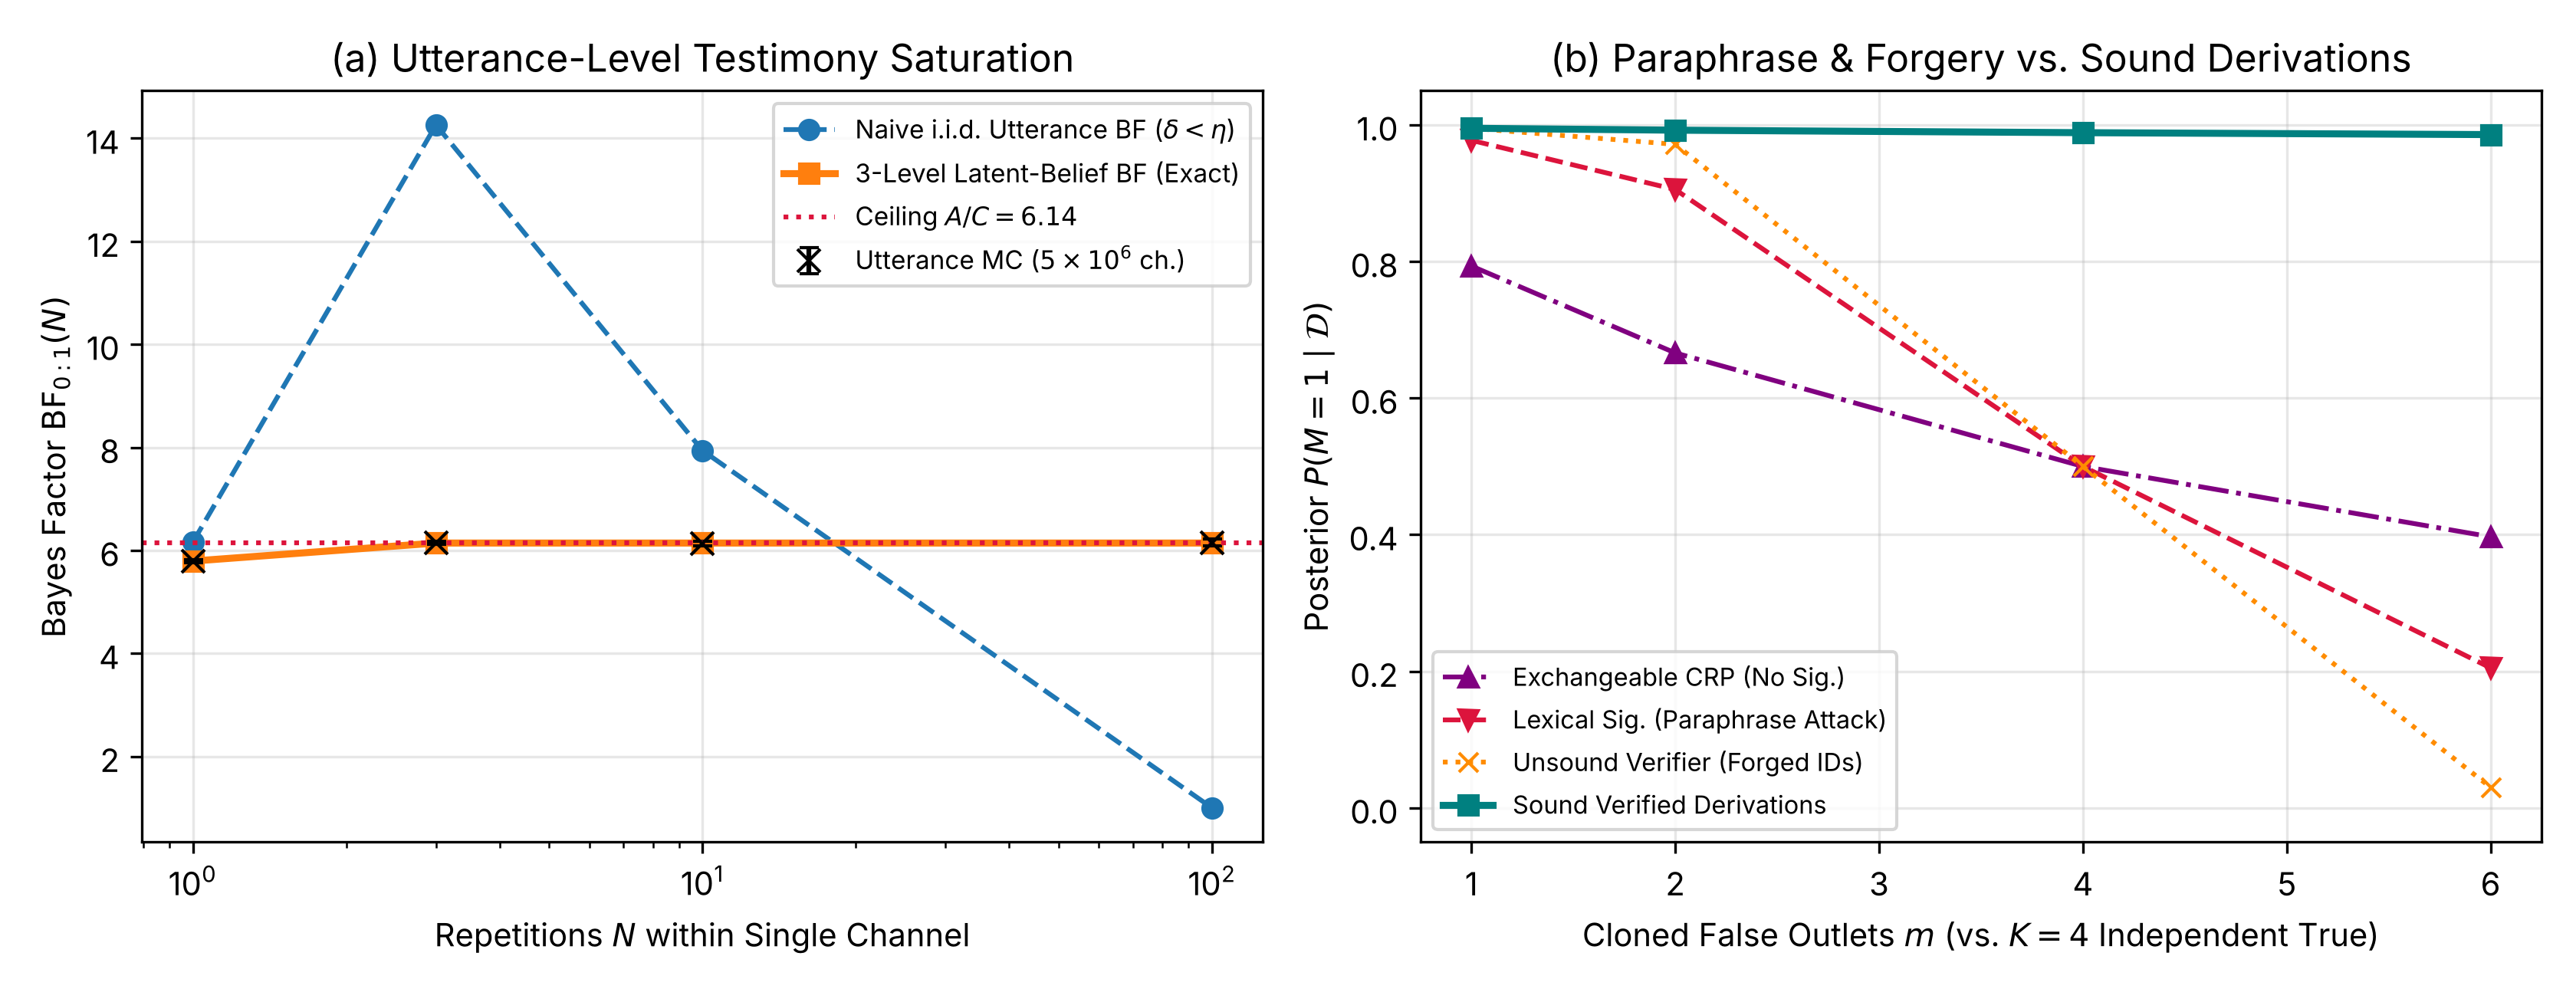
\includegraphics[width=0.94\textwidth]{fig1_testimony_saturation_v8_6.png}
  \caption{(a) Utterance-level Binomial MC and exact 3-level saturation vs.\ naive i.i.d.\ decay; (b) Exact $\mathrm{Bell}(m+4)$ CRP inference under paraphrase and forgery attacks vs.\ sound verified derivations.}
  \label{fig:exp1}
\end{figure}
}{}

\FloatBarrier
\subsection{\texorpdfstring{Experiment 2: $SO(2)$ Breakdown, Harmonic Centring, and Exponent L1}{Experiment 2: SO(2) Breakdown, Harmonic Centring, and Exponent L1}}
\label{sec:exp2}

We construct a $20$-vertex, $30$-edge $SO(2)$ sheaf ($d=2, \nu=3$, default $\gamma_{\mathrm{sh}} = 50$) on the cycle $(i, (i+1)\bmod 20)$ augmented by $10$ chords $(2j, (2j+5)\bmod 20)$, drawing vertex frames $Q_v \in SO(2)$ uniformly and perturbing each edge map by angle $\mathcal{N}(0, \sigma_{\mathrm{map}}^2)$ ($\sigma_{\mathrm{map}} = 0.01\text{ rad}$). The truth is a global section of the \emph{exact} sheaf, $x_{*,v} = Q_v^\top g_{\mathrm{true}}$; every estimator sees only the perturbed maps. Capped probit calibration Eq.~\eqref{eq:reliability_map} ($\omega_{\mathrm{base}} = 160, \hat{\pi}_{\max} = 0.9999, \bar{\omega}_{\max} = \resOmegaCap = \resOmegaCapMult\,\omega_{\mathrm{base}}$) assigns $4$, $10$, and $6$ vertices $\hat{\pi}_v \in \{0.94, 0.84, 0.72\}$, giving $\bar{\omega}_v \in \{\resOmegaTierHigh, \resOmegaTierMid, \resOmegaTierLow\}$ (in the ``Miscalibrated ($4$ noisy)'' row, the last $4$ vertices have true precision $25.0$ while claiming $\hat{\pi}_v = 0.99$). \emph{Colluders} are the first $k$ vertices, which are contiguous on the ring, unless a layout is stated. They report one identical, noiseless false section $Q_v^\top g_{\mathrm{false}}$ and claim precision $500\,\omega_{\mathrm{base}}$. That claim deliberately exceeds the probit cap, modelling an adversary who bypasses calibration; the row labelled ``Capped'' shows the calibrated case. The premise and both bounds of Proposition~\ref{prop:davis_kahan} hold in $\resPropThreePass$ of the $\resPropThreeSeeds$ seeds ($\lambda_2(L_{\widetilde{\mathcal{F}}}) =$ \resPropThreeLamTwo{} $\le \|E_\delta\|_2^2 =$ \resPropThreeWeyl{}; $\|\sin\Theta\|_2 = \resPropThreeSin \le \resPropThreeWedin$ on average), and on one seed the single-outlier discrepancy $\|\hat{x}(\Delta) - \hat{x}_{-u^*}\|_2$ falls from \resThmTwoTen{} ($\Delta=10$) to \resThmTwoThou{} ($\Delta=1000$), consistent with the local $\mathcal{O}(\Delta^{-1})$ rate of Theorem~\ref{thm:robust}(2).

We compare six estimators: (i) \emph{Het.\ Gauss.}, linear Gaussian MAP $\hat{x}_{\mathrm{MAP}}$ using nominal $\bar{\omega}_v$; (ii) \emph{Nom.-Seed-$t$}, Student-$t$ EM initialized at $\hat{x}_{\mathrm{MAP}}$ with nominal $\bar{\omega}_v$; (iii) \emph{Equal-$t$}, Student-$t$ EM using fixed $\omega_{\mathrm{base}}$ throughout; (iv) \emph{Fixed-Warm Het.-$t$}, uncentred Student-$t$ EM initialized at the fixed-scale warm start $x^{(0)}$ ($\omega_{\mathrm{base}}$) and updated with heterogeneous $\bar{\omega}_v$; (v) the \emph{two-stage filter} of Section~\ref{sec:sheaf}, which subtracts the exponent-weighted fit $B\hat{c}$ on $H^0_{\tau_{\mathrm{harm}}}$ (the $d=2$ lowest eigenvectors of $L_{\widetilde{\mathcal{F}}}$), runs (iv) with exponents $s_v$ on the centred data, and adds $B\hat{c}$ back ($s_v \equiv 1$ unless Layer~1 supplies exponents); and (vi) the \emph{three-stage variant}, which is given the generating value $\sigma_{\mathrm{map}} = 0.01$, adds the map-aware coupling $\gamma_\epsilon$ and starts EM from the fit. Every EM runs for at most $35$ iterations and stops earlier only when all seeds of a cell have converged, so the tables report $35$-iteration estimates. With a cap of $500$ the mean RMSE of the $\resCapRmseCells$ Student-$t$ cells of the distance sweep (Table~\ref{tab:exp2_dist}) changes by at most $\resCapRmseMaxRel\%$, and $\resCapCaptChanged$ of the $\resCapCaptCells$ capture percentages of the distance and offset-ratio sweeps change, each by $\resCapCaptMaxDiff$ point. The Stage~1 audit flags a fit whose relative duality gap exceeds $10^{-8}$. It flags $\resStageOneLoose$ of the $\resStageOneFits$ fits behind this section's tables; their largest gap is below \resStageOneGapCert{}, which certifies each fit as the minimizer to that accuracy. RMSE is per coordinate, $\bigl(\frac{1}{|S|d}\sum_{v \in S}\|\hat{x}_v - x_{*,v}\|_2^2\bigr)^{1/2}$ over a vertex set $S$ ($S = V$ unless honest or faulty vertices are named), averaged over seeds. With fault vector $\delta_{\mathrm{fault}} = \frac{\Delta}{\sqrt{2}}(1, -1)^\top$ ($\Delta = 10$ unless stated), we test four placements $(g_{\mathrm{true}}, g_{\mathrm{false}})$: \emph{Truth near $0$} $((1,0)^\top, (1,0)^\top + \delta_{\mathrm{fault}})$, \emph{False claim near $0$} $((1,0)^\top + \delta_{\mathrm{fault}}, (1,0)^\top)$, \emph{Shifted $(20,20)$} $((21,20)^\top, (21,20)^\top + \delta_{\mathrm{fault}})$, and \emph{Symmetric about $0$} $(-\tfrac{1}{2}\delta_{\mathrm{fault}}, +\tfrac{1}{2}\delta_{\mathrm{fault}})$. A seed counts as \emph{captured} when its honest vertices move, on average, more than a quarter of the way toward the false claim.

Tables~\ref{tab:exp2}--\ref{tab:exp2_place} and Figure~\ref{fig:exp2}(a) evaluate estimators (i)--(iv) near the origin. At $\gamma_{\mathrm{sh}} = 50$, $\gamma_0 = 5\times 10^{-4}$ holds across the four modest-radius placements through $k = 9/20$ ($45\%$, $\mathrm{RMSE} = \resWarmNine \pm \resWarmNineSD$ near $0$) and breaks at $k = 10/20$ ($\resWarmTen$) and $k = 11/20$ ($\resWarmEleven$). Heterogeneous precisions help only when they are calibrated: Equal-$t$ is the more accurate filter in the miscalibrated row and degrades more slowly at $k = 10$ (Table~\ref{tab:exp2}). Enforcing the $\resOmegaCapMult\times$ probit cap flips the mean over seeds of $\log P(\hat{x}_{\mathrm{warm}}) - \log P(\hat{x}_{\mathrm{rogue}})$ from $\resGapLegacyUncapNine$ to $\resGapLegacyCapNine$ nats at $\gamma_0 = 0.05, k=9$, and at $\gamma_0 = 5\times 10^{-4}$ gives the warm-started EM endpoint a higher log-posterior than the colluder-seeded endpoint through $k = 8/20$ (mean $\resGapEqCapEight$, smallest $\resGapEqCapEightMin$, vs.\ uncapped mean $\resGapEqUncapEight$ nats), while at $k = 9/20$ (mean $\resGapEqCapNine$ nats) survival relies on Proposition~\ref{prop:warm_start}'s warm-start basin. In each of these five cells all $\resGapSignSeeds$ seeds have the sign of the mean. The gaps compare two EM endpoints; they do not certify a global optimum in any seed. On the exact sheaf the warm-start residuals match the proposition: at $\gamma_{\mathrm{sh}} = 5\times 10^5$ they are $\|r_{\mathrm{fault}}^{(0)}\|_2 = \resPropFourFaultExact$ and $\|r_{\mathrm{hon}}^{(0)}\|_2 = \resPropFourHonExact$, i.e.\ $(1-f_0)\Delta$ and $f_0\Delta$ with $f_0 = 9/20$. With the estimated maps the same residuals read $\resPropFourFaultMod$ and $\resPropFourHonMod$ at the default $\gamma_{\mathrm{sh}} = 50$, $\resPropFourFaultStr$ and $\resPropFourHonStr$ at $5\times 10^5$, and $\resPropFourFaultCollapse$ and $\resPropFourHonCollapse$ at $5\times 10^7$: they leave the proposition's values and head for a collapse onto the origin, because the origin pull of $L_{\widetilde{\mathcal{F}}}$ grows with $\gamma_{\mathrm{sh}}$. In the proposition's limit (exact maps, noiseless honest reports, $\gamma_{\mathrm{sh}} = 10^5$, $\gamma_0 = 10^{-10}$, $\Delta = 10^3$, so $\gamma_0\Delta^2 = 10^{-4}$) the EM iterates for $k=9$ are $f_{1:4} = (\resPropFourTrajEM)$ against $\Psi$'s $(\resPropFourTrajMap)$; with the exponents of Table~\ref{tab:exp2_l1exp}'s second row ($k=12$) they are $(\resPropFourTrajEMExp)$ against $(\resPropFourTrajMapExp)$. The largest gap is \resPropFourMapGap.

\begin{table}[!htbp]
\centering
\caption{Experiment 2(a): Near-origin $SO(2)$ sheaf consensus RMSE ($100$ seeds, $\gamma_0 = 5\times 10^{-4}, \gamma_{\mathrm{sh}}=50, \omega_{\mathrm{base}}=160$).}
\label{tab:exp2}
\footnotesize
\setlength{\tabcolsep}{4.5pt}
\begin{tabular}{@{}lcccc@{}}
\toprule
Scenario ($N=20, d=2, \gamma_0=5\times 10^{-4}$) & Het.\ Gauss. & Nom.-Seed-$t$ & Equal-$t$ & \textbf{Fixed-Warm Het.-$t$} \\
\midrule
\resTabSheafBody
\bottomrule
\end{tabular}
\end{table}

\begin{table}[!htbp]
\centering
\caption{Experiment 2(b): Multi-placement test at $\gamma_{\mathrm{sh}}=50$ ($100$ seeds, $500\times$ colluders, $\Delta=10$; mean RMSE and $\% > 1$).}
\label{tab:exp2_place}
\footnotesize
\setlength{\tabcolsep}{4pt}
\begin{tabular}{@{}llcccc@{}}
\toprule
$\gamma_0$ & Placement & $k=8$ ($40\%$) & $k=9$ ($45\%$) & $k=10$ ($50\%$) & $k=11$ ($55\%$) \\
\midrule
\resTabPlaceBody
\bottomrule
\end{tabular}
\end{table}

\IfFileExists{fig2_sheaf_robustness_v8_6.png}{
\begin{figure}[!htbp]
  \centering
  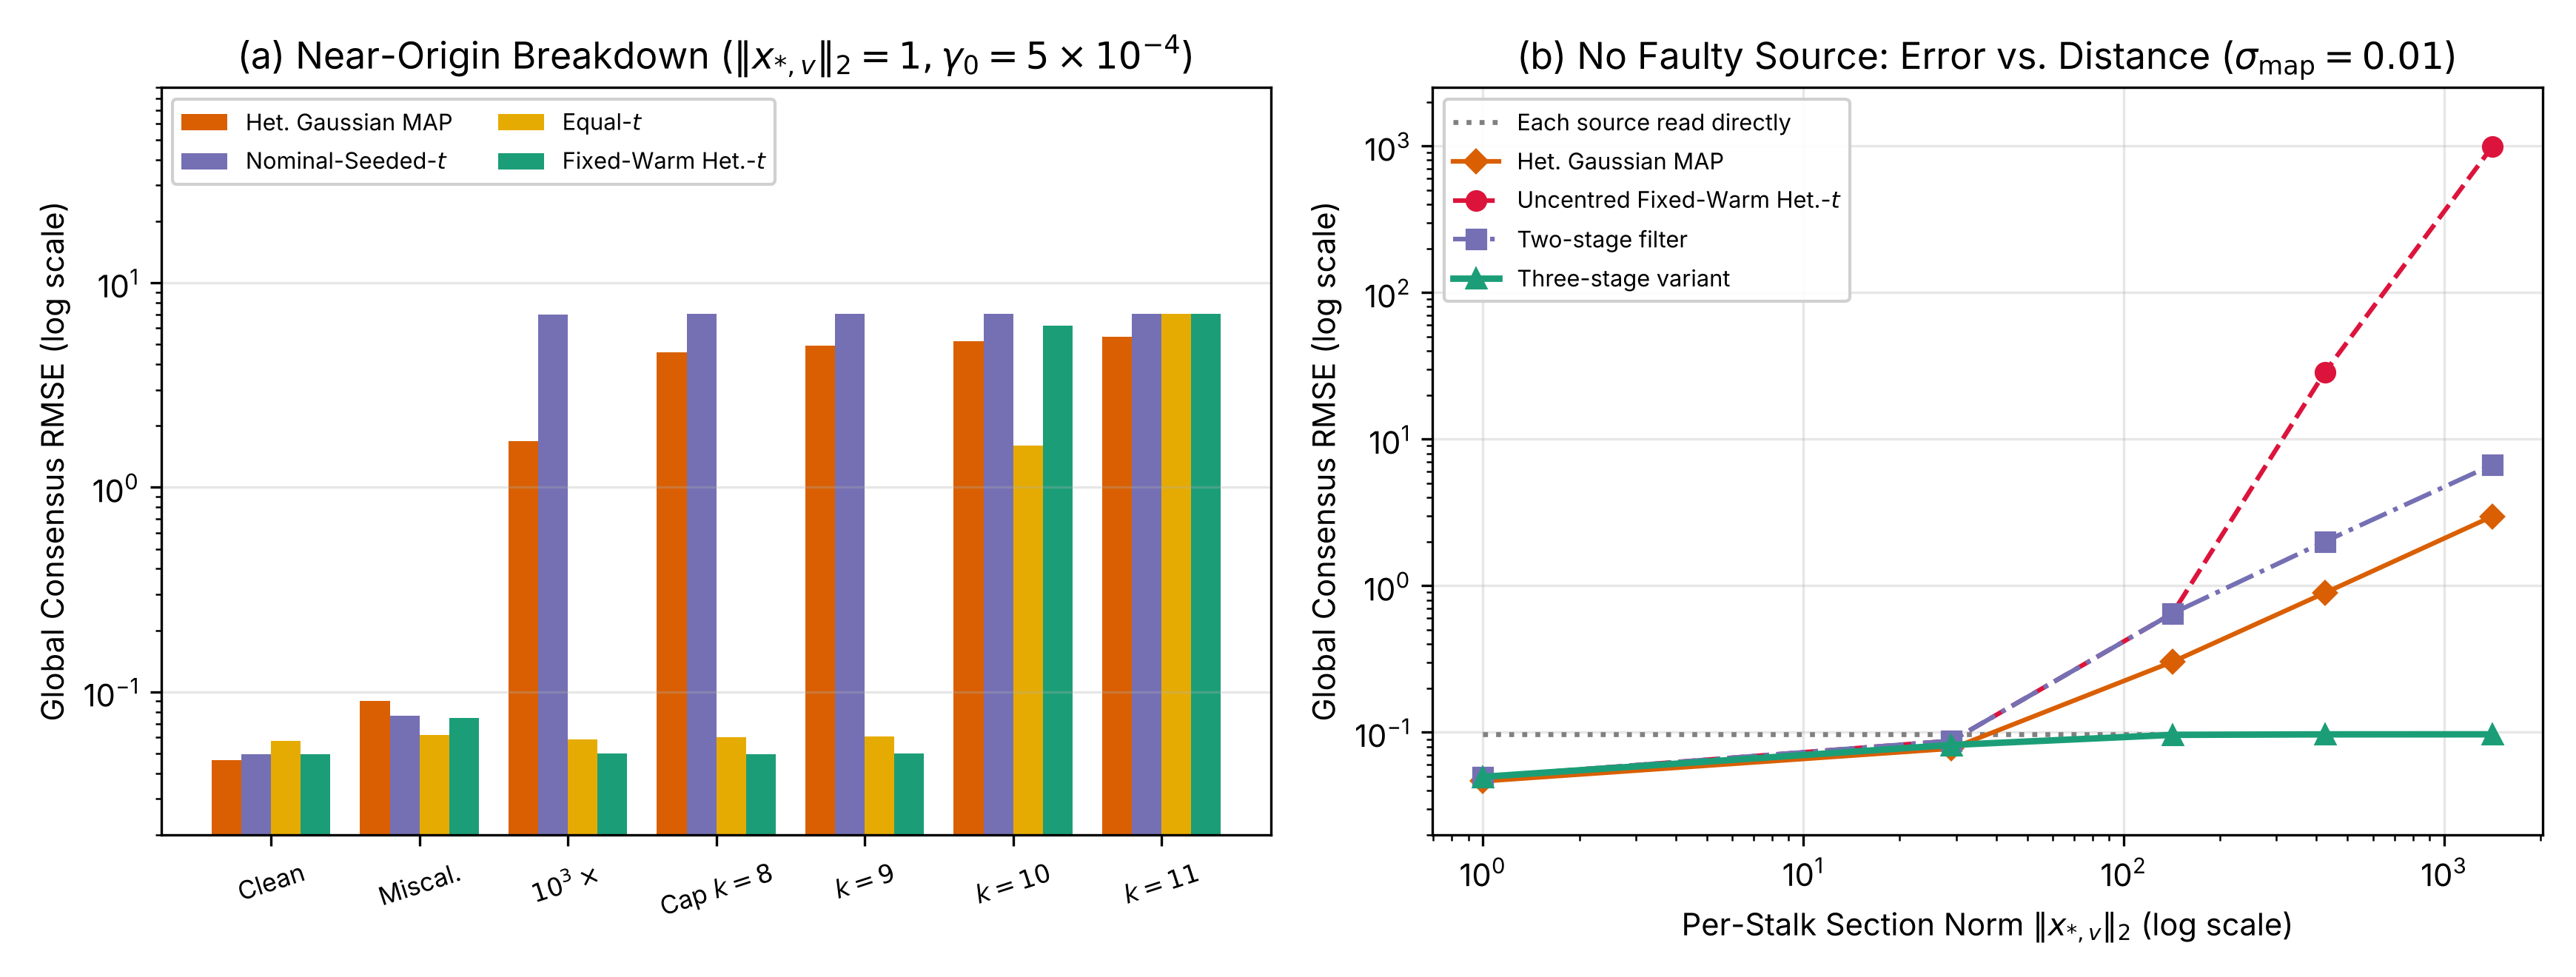
\includegraphics[width=0.96\textwidth]{fig2_sheaf_robustness_v8_6.png}
  \caption{(a) Near-origin breakdown of estimators (i)--(iv) ($\|x_{*,v}\|_2 = 1, \gamma_0=5\times 10^{-4}$); (b) error with no faulty source against section norm, for direct reading, Gaussian pooling, the uncentred filter, the two-stage filter and the three-stage variant.}
  \label{fig:exp2}
\end{figure}
}{}

Table~\ref{tab:exp2_dist} and Figure~\ref{fig:exp2}(b) shift the truth to $g_{\mathrm{true}} = (1,0)^\top + s(1,1)^\top$. With no faulty source, reading each source directly has RMSE $\resRawRMSE$ at every distance, because nothing is pooled. By $(100,100)$ pooling through the estimated maps is worse than that: Gaussian pooling reaches $\resDistGaussHund$ there and $\resDistGaussThreeHund$ at $(300,300)$. The cause is the one named in Section~\ref{sec:sheaf}. At $(300,300)$ the component of the truth outside $H^0_{\tau_{\mathrm{harm}}}$ has mean vertex norm $\resMechNonHarmCoef\,\sigma_{\mathrm{map}}\|x_{*,v}\|_2$, and the noiseless warm-start residual splits into mean vertex norms of $\resMechWarmHarm$ (harmonic part) and $\resMechWarmNonHarm$ (non-harmonic part), against Student-$t$ core half-widths of $\resMechCoreMin$--$\resMechCoreMax$. Honest data therefore sit in the tails, and the uncentred filter collapses toward the origin (RMSE $\resDistWarmThreeHund$ at $(300,300)$ and $\resDistWarmThou$ at $(1000,1000)$). Stage~1 centring stops the collapse ($\resDistCentThreeHund$ and $\resDistCentThou$) but leaves a per-coordinate error floor near $\resFloorCentCoef\,\sigma_{\mathrm{map}}\|x_{*,v}\|_2$, against $\resFloorGaussCoef\,\sigma_{\mathrm{map}}\|x_{*,v}\|_2$ for Gaussian pooling. The three-stage variant returns to the direct-reading level ($\resDistThreeHund$, $\resDistThreeThreeHund$ and $\resDistThreeThou$ at the three largest shifts), because at those shifts $\gamma_\epsilon$ lies far below every $\bar{\omega}_v$, which decouples the edges.

With $k=9$ colluders at $\Delta = 10$, the two-stage filter is not captured within $29$ units of the origin, but $\resDistNineCaptHund\%$ of seeds are captured at $(100,100)$ and $\resDistNineCaptThreeHund\%$ at $(300,300)$. There $\Delta$ is $\resDistRatioThreeHund$ times $\sigma_{\mathrm{map}}\|x_{*,v}\|_2$, honest vertices move $\resDistNineDriftThreeHund\%$ of the way on average, and the RMSE is $\resDistNineCentThreeHund$ against $\resDistNineOracleThreeHund$ for an oracle that drops the nine colluders. Table~\ref{tab:exp2_ratio} sweeps the offset in units of $\sigma_{\mathrm{map}}\|x_{*,v}\|_2$. At $1.5$ times, $\resRatioAdjLowMin\%$--$\resRatioAdjLowMax\%$ of seeds are captured with adjacent colluders; no seed is captured only from $\resRatioClearAdj$ times (adjacent) or $\resRatioClearSca$ times (scattered). For the three-stage variant, whose edges are nearly decoupled at both distances, the worst cell is $\resRatioThreeAdjMax\%$ of seeds captured with adjacent colluders and $\resRatioThreeScaMax\%$ with scattered ones, and no seed is captured from $\resRatioThreeScaClear$ times. These thresholds are grid values on one graph at two shifts, not a general margin. The scattered rows of the three-stage variant are not monotone in the offset (no capture at $1.5$ times, the worst cell at $2.5$ times), and a cell with no capture in $100$ seeds bounds its capture probability only by $\resZeroCaptUpper\%$ (one-sided $95\%$). The variant's cost falls on the faulty vertices themselves: the weakened coupling no longer overrules them at moderate offsets, so at $(300,300)$ their RMSE is $\resDistNineThreeFaultThreeHund$, essentially the offset $\Delta/\sqrt{2}$ per coordinate, and the all-vertex RMSE is $\resDistNineThreeAllThreeHund$ although the honest vertices stay at $\resDistNineThreeHonThreeHund$.

Across $\gamma_{\mathrm{sh}} \in \{50, 500, 5000\}$ (Table~\ref{tab:exp2_coup}), the uncentred filter breaks on non-origin placements at $\gamma_{\mathrm{sh}} \ge 500$, whereas the two-stage filter's worst cell across all four placements is $\resCoupCentMaxEightNine\%$ of seeds failing for $k \in \{8, 9\}$, with $\resCoupCentTenMin\%$--$\resCoupCentTenMax\%$ failing at $k = 10$; the three-stage variant's worst cell for $k \in \{8, 9\}$ is $\resCoupThreeMaxEightNine\%$ as well. At $\gamma_{\mathrm{sh}} = 5$ the warm start no longer pools: the best cell of the uncentred and two-stage filters is $\resCoupCentWeakMinEightNine\%$ of seeds failing, while the three-stage variant, which starts from the Stage~1 fit, keeps its worst cell for $k \in \{8, 9\}$ at $\resCoupThreeWeakMaxEightNine\%$. Those failures are captures of the honest vertices, not errors confined to the faulty ones: over the cells with $k \in \{8, 9\}$ the two-stage filter's lowest capture rate at $\gamma_{\mathrm{sh}} = 5$ is $\resIngrTwoWeakCaptMin\%$ of seeds (Table~\ref{tab:exp2_ingr}).

\begin{table}[!htbp]
\centering
\caption{Experiment 2(c): Distance sweep ($100$ seeds, $\gamma_0 = 5\times 10^{-4}, \gamma_{\mathrm{sh}} = 50$). Left block: mean RMSE with no faulty source. Right block: $k=9$ colluders ($500\times$, $\Delta = 10$) with the two-stage filter's mean RMSE and percent of seeds captured, an oracle that drops the colluders, and the three-stage variant's RMSE over honest vertices and percent captured. Columns: direct reading, Gaussian pooling (i), uncentred filter (iv), two-stage filter (v), three-stage variant (vi).}
\label{tab:exp2_dist}
\scriptsize
\setlength{\tabcolsep}{2.6pt}
\begin{tabular}{@{}lrcccccccccc@{}}
\toprule
 & & \multicolumn{5}{c}{$k=0$ (no faulty vertex)} & \multicolumn{5}{c}{$k=9$ ($45\%$), $\Delta = 10$} \\
\cmidrule(lr){3-7}\cmidrule(l){8-12}
Shift & $\|x_{*,v}\|_2$ & Direct & Gauss. & Uncent. & \textbf{Two-st.} & Three-st. & \textbf{Two-st.} & capt.\,\% & Oracle & Three-st.\ hon. & capt.\,\% \\
\midrule
\resTabDistBody
\bottomrule
\end{tabular}
\end{table}

\begin{table}[!htbp]
\centering
\caption{Experiment 2(d): Offset-ratio sweep ($100$ seeds, $k=9$, $\gamma_{\mathrm{sh}} = 50$): percent of seeds captured, by offset $\Delta$ as a multiple of the map discrepancy $\sigma_{\mathrm{map}}\|x_{*,v}\|_2$, for adjacent ($0,\dots,8$) and scattered (even) colluders.}
\label{tab:exp2_ratio}
\footnotesize
\setlength{\tabcolsep}{4.5pt}
\begin{tabular}{@{}lllcccccccc@{}}
\toprule
 & & & \multicolumn{8}{c}{$\Delta \,/\, (\sigma_{\mathrm{map}}\|x_{*,v}\|_2)$} \\
\cmidrule(l){4-11}
Filter & Layout & Shift & $1.5$ & $2.5$ & $5$ & $7.5$ & $10$ & $15$ & $20$ & $30$ \\
\midrule
\resTabRatioBody
\bottomrule
\end{tabular}
\end{table}

\begin{table}[!htbp]
\centering
\caption{Experiment 2(e): Coupling-strength sweep ($100$ seeds, $\gamma_0 = 5\times 10^{-4}, 500\times$ colluders, $\Delta = 10$): percentage of seeds with $\mathrm{RMSE} > 1$ before and after $H^0_{\tau_{\mathrm{harm}}}$ centring.}
\label{tab:exp2_coup}
\footnotesize
\setlength{\tabcolsep}{4pt}
\begin{tabular}{@{}rlcccccccc@{}}
\toprule
 & & \multicolumn{4}{c}{Uncentred Fixed-Warm Het.-$t$ (iv)} & \multicolumn{4}{c}{\textbf{Two-stage filter (v)}} \\
\cmidrule(lr){3-6}\cmidrule(l){7-10}
$\gamma_{\mathrm{sh}}$ & Placement & $k=8$ & $k=9$ & $k=10$ & $k=11$ & $k=8$ & $k=9$ & $k=10$ & $k=11$ \\
\midrule
\resTabCoupBody
\bottomrule
\end{tabular}
\end{table}

Tables~\ref{tab:exp2_sweep}--\ref{tab:exp2_capt} map the finite-$\gamma_{\mathrm{sh}}$ core-to-tail transition over $(k, \Delta)$ and graph topology near the origin. For the two-stage filter, $9$ contiguous colluders ($0,\dots,8$) have a small boundary cut to honest vertices and drag honest states by $\resCaptAdjNineLowMin\%$--$\resCaptAdjNineLowMax\%$ of $\Delta$ for $\Delta \le 2.0$ before dropping to $\resCaptAdjNineAtTwoFive\%$ at $\Delta = 2.5$, whereas $9$ scattered colluders (even vertices) leave the honest states in place ($\resCaptScaNineAtOne\%$ drift) from $\Delta = 1.0$. The two layouts differ in more than the cut ($7$ against $27$ of the $30$ edges): the contiguous block also replaces all four high-precision vertices, the scattered set two of them. The contrast survives when that difference is removed. With every honest precision set to $\omega_{\mathrm{base}}$, the contiguous block still drags honest states by $\resCaptEqAdjNineLowMin\%$--$\resCaptEqAdjNineLowMax\%$ of $\Delta$ for $\Delta \le 1.5$ ($\resCaptEqAdjNineAtTwo\%$ at $\Delta = 2.0$), and the scattered set by $\resCaptEqScaNineAtOne\%$ at $\Delta = 1.0$. The tiers therefore move the contiguous block's transition but do not create it. The layout rows of Table~\ref{tab:exp2_ratio} carry the same confound and were not rerun. Starting EM from the Stage~1 fit shrinks this zone: for the contiguous block the three-stage variant leaves $\resCaptThreeAdjNineAtOne\%$ drift at $\Delta = 1.0$ and $\resCaptThreeAdjNineAtOneTwoFive\%$ at $\Delta = 1.25$.

Layer~1 enters through the exponents. The inverse cluster sizes $\hat{s}_v$ are computed exactly: a dynamic programme over the counts of exchangeable sources sums over all set partitions (with Experiment~1's $\alpha_{\mathrm{CRP}}$, $V_{\mathrm{sig}}$, $p_{\mathrm{unv}}$, $\mu_{\mathrm{drop}}$ and $\epsilon_{\mathrm{ind}}$), and it agrees to $10^{-12}$ with exhaustive enumeration of the $\resLOneExactTestBell$ partitions of a nine-source pattern. Layer~1 sees the signatures only, so it cannot separate an unverified clone from an unverified independent source. Table~\ref{tab:exp2_l1exp} lists $\hat{s}$ and the resulting $S_{\mathrm{fault}}$ and $S_{\mathrm{hon}}$ for five signature patterns, and compares two uses of them. Both apply \emph{tier capping} first: an unverified source ($W_v = 0$) is assigned the lowest calibrated tier, $\hat{\pi}_v = 0.72$. Both then run the weighted Stage~1 and the warm start of the two-stage filter and differ only in the EM weights: \emph{precision division} rescales $\bar{\omega}_v$ by $\hat{s}_v$, whereas the two-stage filter raises each potential to the power $s_v = \hat{s}_v$. Twelve unverified clones receive $\hat{s} = \resLOneCloneShat$ each, a total of $\resLOneCloneSum$ rather than $1$, while twelve clones sharing one verified ID total $\resLOneSharedSum$. When $12$ clones and $6$ honest domains are \emph{both} unverified alongside $2$ verified honest domains, every unverified source receives the same exponent, $\resLOneMixClone$, and each verified source $\resLOneMixHonVer$, so $S_{\mathrm{fault}} = \resLOneMixSf < S_{\mathrm{hon}} = \resLOneMixSh$. Precision division is then captured ($\resLOneMixDiv$, and $\resLOneMixDivUnc$ without centring) because tail precisions cancel, whereas the exponents recover $\resLOneMixExp$ (also rescuing $k=3, \Delta=0.4$ shared verified IDs: $\resLOneSmallSharedExp$ vs.\ $\resLOneSmallSharedDiv$). Forged distinct IDs and an all-unverified majority ($S_{\mathrm{fault}} = \resLOneAllSf > S_{\mathrm{hon}} = \resLOneAllSh$) fail, as Eq.~\eqref{eq:em_dynamics} predicts.

Table~\ref{tab:exp2_bound} locates the boundary by varying the number $k$ of unverified clones and $h$ of verified honest sources. The outcome follows the sign of $S_{\mathrm{fault}} - S_{\mathrm{hon}}$ in all $\resBoundRuleCells$ cells, each of which is captured in every seed or in none. At $N = 20$ an unverified majority of $12$, $14$ or $16$ clones is therefore outvoted only with $\resBoundFirstHTwelve$, $\resBoundFirstHFourteen$ or $\resBoundFirstHSixteen$ verified honest sources. The margin is thin: the first protected cell has $S_{\mathrm{fault}}/S_{\mathrm{hon}} = \resBoundFirstRatioTwelve$ at $k=12$, $\resBoundFirstRatioFourteen$ at $k=14$ and $\resBoundFirstRatioSixteen$ at $k=16$. The cell nearest parity, $(k,h) = (16,3)$, has $S_{\mathrm{fault}}/S_{\mathrm{hon}} = \resBoundNearRatio$ and is captured in $\resBoundNearCapt\%$ of seeds; it stays captured at $\gamma_{\mathrm{sh}} = 500$ ($\resBoundNearCaptStrong\%$) and under the three-stage variant ($\resBoundNearCaptThree\%$). Tier capping lowers the precision of unverified sources only, but that plays no part here. For $k = 14$ and $k = 16$ every honest vertex already sits in the lowest tier, and with every source assigned that tier all $\resBoundFlatSame$ cells are unchanged, so the exponents alone decide the table. A heuristic accounts for the count. Eq.~\eqref{eq:deriv_sig_lik} cannot separate unverified sources, so the $m_0 = N - h$ of them share a total exponent close to the expected number of blocks of a Chinese Restaurant Process with concentration $\alpha_{\mathrm{CRP}}\,p_{\mathrm{unv}}$, namely $\sum_{j=0}^{m_0-1} \alpha_{\mathrm{CRP}}\,p_{\mathrm{unv}} / (\alpha_{\mathrm{CRP}}\,p_{\mathrm{unv}} + j)$, which grows as $\ln m_0$, while each verified source keeps an exponent near one. At a fixed clone fraction the number of verified honest sources needed for $S_{\mathrm{fault}} < S_{\mathrm{hon}}$ should therefore grow only logarithmically in $N$; no experiment here tests that beyond $N = 20$.

Table~\ref{tab:exp2_comb} runs centring and exponents together on the second pattern as the offset grows. With an \emph{unweighted} Stage~1 fit the $12$ clones capture the spatial median, and the filter that follows is captured in $\resCombUnwTruthTwenty\%$ of seeds at $\Delta = 20$ and $\resCombUnwTruthForty\%$ at $\Delta = 40$: a larger lie succeeds where a smaller one fails. Exponents without centring fail the same way when the false claim is the one nearer the origin ($\resCombExpMirrorForty\%$ at $\Delta = 40$). For the two-stage filter, whose Stage~1 carries the exponents, the worst cell is $\resCombTwoMax\%$ of seeds captured, and for the three-stage variant $\resCombThreeMax\%$.

Finally, Table~\ref{tab:exp2_ingr} takes the three-stage variant apart. It differs from the two-stage filter in the EM start and in the edge coupling, and the table crosses the two (with $s_v \equiv 1$; each warm start is computed with its own arm's coupling). The fit start is what survives weak coupling: at $\gamma_{\mathrm{sh}} = 5$ the worst cell of the two arms started from the fit is $\resIngrFitWeakFailMax\%$ of seeds failing, while the best cell of the two warm-started arms is $\resIngrWarmWeakFailMin\%$, with honest vertices captured in at least $\resIngrWarmWeakCaptMin\%$ of seeds. The map-aware coupling is what restores accuracy far from the origin: with it the no-fault RMSE at $(1000,1000)$ is $\resIngrMapNoFaultThou$ even from the warm start, the direct-reading level, against $\resIngrFitNoFaultThou$ for the fit start with uniform coupling. Neither change stands alone. The fit start with uniform coupling keeps that far-field error and is captured in up to $\resIngrFitLowCaptMax\%$ of seeds at offset ratios below five. The map-aware coupling with the warm start is captured in up to $\resIngrMapHighCaptMax\%$ of seeds at ratios of five and more, and at the shifted placement it fails in $\resIngrMapShiftedFailEight\%$ of seeds at $k = 8$ and $\resIngrMapShiftedFailNine\%$ at $k = 9$ even at $\gamma_{\mathrm{sh}} = 50$ (worst cell at the other placements: $\resIngrMapElseFailMax\%$). There the formula lowers the edge couplings to $\resIngrGammaShifted$ on average, and the two-stage filter with a uniform coupling of that size fails as often ($\resIngrUnifShiftedFailEight\%$ and $\resIngrUnifShiftedFailNine\%$). A weakened edge is therefore what the warm start cannot survive, so the map-aware coupling needs the fit start.

The last two rows give the variant a wrong scale. With $\sigma_{\mathrm{map}}$ halved the edges stay too stiff far out: the no-fault RMSE at $(1000,1000)$ rises to $\resIngrHalfNoFaultThou$, and up to $\resIngrHalfLowCaptMax\%$ of seeds are captured at offset ratios below five, against $\resIngrThreeLowCaptMax\%$ with the true value. With $\sigma_{\mathrm{map}}$ doubled the worst cell of the ratio sweep is $\resIngrDoubleCaptMax\%$ of seeds captured and the far-field error stays at the direct-reading level ($\resIngrDoubleNoFaultThou$), but the edges loosen where pooling still helps: at $(20,20)$ the no-fault RMSE rises from $\resIngrThreeNoFaultTwenty$ to $\resIngrDoubleNoFaultTwenty$, toward the direct-reading $\resRawRMSE$. An overestimate thus gives up part of the gain from pooling, whereas an underestimate, although it lowers the no-fault error at $(20,20)$, gives up accuracy far from the origin and raises capture at small ratios. No experiment here estimates $\sigma_{\mathrm{map}}$ from the data, so the variant's advantages rest on a scale that the two-stage filter does not use.

\begin{table}[!htbp]
\centering
\caption{Experiment 2(f): Single-fault magnitude sweep across the Student-$t$ core-to-tail transition ($100$ seeds).}
\label{tab:exp2_sweep}
\footnotesize
\setlength{\tabcolsep}{5pt}
\begin{tabular}{@{}lcccc@{}}
\toprule
Fault Regime ($\gamma_0 = 5\times 10^{-4}$) & Het.\ Gauss. & Nom.-Seed-$t$ & Equal-$t$ & \textbf{Fixed-Warm Het.-$t$} \\
\midrule
\resTabSweepBody
\bottomrule
\end{tabular}
\end{table}

\begin{table}[!htbp]
\centering
\caption{Experiment 2(g): Capture map ($100$ seeds, $\gamma_0 = 5\times 10^{-4}, \gamma_{\mathrm{sh}} = 50, 500\times$ colluders): mean honest-vertex drift toward the false claim in $\%$ of $\Delta$ ($0$ = honest vertices unmoved, $100$ = captured) for adjacent vs.\ scattered colluders.}
\label{tab:exp2_capt}
\footnotesize
\setlength{\tabcolsep}{4pt}
\begin{tabular}{@{}llcccccccccc@{}}
\toprule
Filter & Layout & $k$ & $\Delta=0.4$ & $0.8$ & $1.0$ & $1.25$ & $1.5$ & $2.0$ & $2.5$ & $5.0$ & $10$ \\
\midrule
\resTabCaptBody
\bottomrule
\end{tabular}
\end{table}

\begin{table}[!htbp]
\centering
\caption{Experiment 2(h): Layer-1 signature scenarios ($100$ seeds, exact $\hat{s}_v$): exponents at $k=12$ and mean RMSE for precision division against the two-stage filter with exponents $s_v = \hat{s}_v$. Both arms use the same weighted Stage~1 and warm start.}
\label{tab:exp2_l1exp}
\footnotesize
\setlength{\tabcolsep}{3.5pt}
\begin{tabular}{@{}lccccccc@{}}
\toprule
 & \multicolumn{3}{c}{Exponents at $k=12$} & \multicolumn{2}{c}{$k=12$, $\Delta=10$} & \multicolumn{2}{c}{$k=3$, $\Delta=0.4$} \\
\cmidrule(lr){2-4}\cmidrule(lr){5-6}\cmidrule(l){7-8}
Signatures seen by Layer~1 & $\hat{s}_{\mathrm{clone}}$ & $S_{\mathrm{fault}}$ & $S_{\mathrm{hon}}$ & Prec.\ div. & \textbf{Two-stage} & Prec.\ div. & \textbf{Two-stage} \\
\midrule
\resTabLOneExpBody
\bottomrule
\end{tabular}
\end{table}

\begin{table}[!htbp]
\centering
\caption{Experiment 2(i): Verified-source boundary for the two-stage filter ($100$ seeds, $\Delta = 10$, exact $\hat{s}_v$): $k$ unverified clones, $h$ verified honest sources, all other honest sources unverified. Cells give $S_{\mathrm{fault}}/S_{\mathrm{hon}}$ and the percent of seeds captured; at $(k,h) = (16,3)$ the ratio is $\resBoundNearRatio$.}
\label{tab:exp2_bound}
\footnotesize
\setlength{\tabcolsep}{4pt}
\begin{tabular}{@{}lccccc@{}}
\toprule
Clones & $h=0$ & $h=1$ & $h=2$ & $h=3$ & $h=4$ \\
\midrule
\resTabBoundBody
\bottomrule
\end{tabular}
\end{table}

\begin{table}[!htbp]
\centering
\caption{Experiment 2(j): Centring and exponents together under a clone majority ($100$ seeds; $12$ unverified clones, $6$ unverified and $2$ verified honest sources): percent of seeds captured as the offset grows.}
\label{tab:exp2_comb}
\footnotesize
\setlength{\tabcolsep}{5pt}
\begin{tabular}{@{}llccccc@{}}
\toprule
Placement & Filter & $\Delta=10$ & $20$ & $40$ & $80$ & $160$ \\
\midrule
\resTabCombBody
\bottomrule
\end{tabular}
\end{table}

\begin{table}[!htbp]
\centering
\caption{Experiment 2(k): Ingredients of the three-stage variant ($100$ seeds, $\gamma_0 = 5\times 10^{-4}$, $s_v \equiv 1$). The first four rows cross the EM start with the edge coupling; the last two give the three-stage variant half and twice the generating $\sigma_{\mathrm{map}}$. Columns~2--4: $k \in \{8, 9\}$ colluders ($500\times$, $\Delta = 10$) at the four placements, as the range over those eight cells of the percent of seeds with $\mathrm{RMSE} > 1$ and of seeds captured. Columns~5--8 use $\gamma_{\mathrm{sh}} = 50$. Columns~5--6: mean RMSE with no faulty source (direct reading: $\resRawRMSE$). Columns~7--8: the largest percent of seeds captured over the cells of the sweep of Table~\ref{tab:exp2_ratio} ($k = 9$, both layouts, both shifts) with offset ratio $\Delta/(\sigma_{\mathrm{map}}\|x_{*,v}\|_2)$ below five and from five up; the ratio always uses the generating $\sigma_{\mathrm{map}}$.}
\label{tab:exp2_ingr}
\footnotesize
\setlength{\tabcolsep}{4pt}
\begin{tabular}{@{}lccccccc@{}}
\toprule
 & \multicolumn{2}{c}{$\gamma_{\mathrm{sh}} = 5$} & $\gamma_{\mathrm{sh}} = 50$ & \multicolumn{2}{c}{No-fault RMSE at} & \multicolumn{2}{c}{Worst \% captured} \\
\cmidrule(lr){2-3}\cmidrule(lr){4-4}\cmidrule(lr){5-6}\cmidrule(l){7-8}
EM start, coupling & \% fail & \% capt. & \% fail & $(20,20)$ & $(1000,1000)$ & ratio $< 5$ & ratio $\ge 5$ \\
\midrule
\resTabIngrBody
\bottomrule
\end{tabular}
\end{table}

\FloatBarrier
\subsection{\texorpdfstring{Experiment 3: Dial-Free Spacetime Sheaves and Two-Step Annulus Power}{Experiment 3: Dial-Free Spacetime Sheaves and Two-Step Annulus Power}}
\label{sec:exp3}

On a $3$-observer spacetime triangle $E_X = \{(0,1), (1,2), (0,2)\}$ ($d=2, \sigma_y = 0.01, \gamma_0 = 0.10$) with rapidities $\varphi = (0, 0.5 s_{\mathrm{rap}}, 1.1 s_{\mathrm{rap}})$ ($s_{\mathrm{rap}} \in \{0.05, 0.30, 0.60, 0.85\}$, matched Galilean speeds $v_{\mathrm{Gal}} = (0, \frac{0.5}{1.1}\beta_{\max}, \beta_{\max})$, and $M_{\mathrm{ev}} = 20$ events drawn from $\mathcal{N}(0, I_2)$), Table~\ref{tab:exp3} and Figure~\ref{fig:exp3} compare fixed-$\gamma_{\mathrm{sh}}$ analytical $\E[\log\BF]$ against dial-free profiled and $\mathrm{HalfCauchy}(50)$-marginalized per-event $\log\BF$ ($100$ seeds) and matched-$\beta_{\max}$ Galilean controls. Under $\mathrm{HalfCauchy}(50)$, per-event $\log\BF$ rises from $\resSpaceHCmin$ at $0.05c$---where the simultaneity shift $-\gamma\beta_{\max} x \approx 0.055 \approx 5.5\sigma_y$ is resolved by $\sigma_y = 0.01$ clocks (raising sensor noise to $\sigma_y = 0.10 > \beta_{\max}$ lowers the $0.05c$ $\mathrm{HalfCauchy}$ $\log\BF$ to $\resSpaceNoisyCtrl \pm \resSpaceNoisyCtrlSD$ nats per event, so that a single event no longer separates the sheaves \cite{nozick2001invariances}; a $20$-event dataset still carries $\resSpaceNoisyCtrlTotal$ nats on average, and replication accumulates it)---up to $\resSpaceHCmax$ at $0.73c$. Across $2{,}000$ single events at $\gamma_{\mathrm{sh}} = 50$, medians ($\resSpaceMedA$, $\resSpaceMedB$, $\resSpaceMedC$, $\resSpaceMedD$), IQRs ($\resSpaceIQRA$, $\resSpaceIQRB$, $\resSpaceIQRC$, $\resSpaceIQRD$), and uninformative shares $|\log\BF|<1$ ($\resSpaceUninfA\%$, $\resSpaceUninfB\%$, $\resSpaceUninfC\%$, $\resSpaceUninfD\%$) reflect where each event lies. Without noise the single-event $\log\BF$ is a constant plus a quadratic form in the event's base-frame coordinates $(ct, x)$ whose smaller eigenvalue is at most $\resSpaceFormRatioMax\%$ of the larger, so an event is uninformative when its coordinate along one direction is small. That direction is the spatial axis at $0.05c$ (spatial component $\resSpaceFormXLow$), as the first-order misfit $-\gamma\beta x$ suggests, and it tilts toward the time axis by $0.73c$ ($\resSpaceFormXHigh$). It is a direction in the event plane, not a common section space of the two sheaves. At $0.73c$, sweeping $\gamma_{\mathrm{sh}} \in \{5, 50, 500\}$ ($\gamma_0 = 0.10$) yields $\E[\log\BF] \in \{\resSwGshFiveBF, \resSwGshFiftyBF, \resSwGshFiveHundBF\}$ (share of the expected Galilean quadratic term outside its kernel mode that the $\lambda_2$ eigenmode carries: $\{\resSwGshFiveLam\%, \resSwGshFiftyLam\%, \resSwGshFiveHundLam\%\}$), while $\gamma_0 \in \{10^{-1}, 10^{-3}, 10^{-6}\}$ ($\gamma_{\mathrm{sh}}=50$) shifts Occam across $\{\resSwGzeroTenthOcc, \resSwGzeroMilliOcc, \resSwGzeroMicroOcc\}$ nats ($\E[\log\BF] \in \{\resSwGzeroTenthBF, \resSwGzeroMilliBF, \resSwGzeroMicroBF\}$).

To test Section~\ref{sec:sheaf}'s two-step Hodge rule, we triangulate an annulus between inner cycle $(0,1,2)$ and outer cycle $(3,4,5)$ with $12$ edges and $6$ triangles ($\dim\im\delta^0 = 5$, $\dim\im(\delta^1)^\top = 6$, $\dim H^1 = 1$), adding $\mathcal{N}(0, \sigma_{\mathrm{edge}}^2)$ noise ($\sigma_{\mathrm{edge}} = 0.05$) to baseline gradient $y_{\mathrm{base}} = \delta^0 v_0$ with $v_0 = (0,\allowbreak 0.4,\allowbreak -0.3,\allowbreak 0.5,\allowbreak -0.2,\allowbreak 0.1)^\top$ and testing at $\alpha = 1\%$ against $\chi^2_6$ (curl) and $\chi^2_1$ ($H^1$) thresholds. Because $\Pcurl$ and $\Pharm$ are orthogonal projectors, the two statistics are independent non-central $\chi^2$ variables, so every rate in Table~\ref{tab:annulus} is exact. A single boundary fault on $(0,1)$ projects onto both curl and $H^1$. At unit size the rule calls it local in $\resAnnEdgeUnitLocal\%$ of draws; at $+0.2$ it is called local in $\resAnnEdgeModLocal\%$, mislabelled global in $\resAnnEdgeModGlobal\%$ and missed in $\resAnnEdgeModNone\%$. A curl-free radial branch cut across $\{(0,1), (0,4), (3,4)\}$ leaves the curl test at its null rate ($\resAnnCutModLocal\%$) and is called global in $\resAnnCutModGlobal\%$ of draws at $+0.2$ and $\resAnnCutUnitGlobal\%$ at $+1.0$. A mixed fault (the cut plus spoke $(1,4)$) receives a single label: local in $\resAnnMixModLocal\%$ and global in $\resAnnMixModGlobal\%$ of draws at $+0.2$, and local in $\resAnnMixUnitLocal\%$ at unit size, where the cut goes unreported. With no fault the rule raises some alarm in $\resAnnNullAlarm\%$ of draws, twice the level of either test.

\begin{table}[!htbp]
\centering
\caption{Experiment 3(a): $2\times 2$ spacetime sheaves ($100$ seeds $\times 20$ events, $\sigma_y = 0.01, \gamma_0 = 0.10$) comparing fixed-$50$ $\E[\log\BF]$ against a dial-free profiled log-likelihood ratio and a $\mathrm{HalfCauchy}(50)$ per-event $\log\BF$.}
\label{tab:exp3}
\footnotesize
\setlength{\tabcolsep}{4pt}
\begin{tabular}{@{}cccccc@{}}
\toprule
$\beta_{\max}$ & $\lambda_2(L_{\mathcal{F}_{\mathrm{Gal}}})$ & Fixed-$50$ $\E[\log\BF]$ & Profiled log-LR (Lor.) & \textbf{Half-Cauchy (Lor.)} & Matched Gal.\ Ctrl \\
\midrule
\resTabSpaceBody
\bottomrule
\end{tabular}
\end{table}

\begin{table}[!htbp]
\centering
\caption{Experiment 3(b): Two-step Hodge rule on the triangulated annulus ($\sigma_{\mathrm{edge}} = 0.05$, $\alpha = 1\%$): noise-free projections of each signal $s$, exact rejection rates of the $\chi^2_6$ curl and $\chi^2_1$ $H^1$ tests, and exact rates of the rule's three decisions (all rates in $\%$; bold marks the correct decision for a single fault).}
\label{tab:annulus}
\footnotesize
\setlength{\tabcolsep}{3.5pt}
\begin{tabular}{@{}lccccccc@{}}
\toprule
 & \multicolumn{2}{c}{Signal} & \multicolumn{2}{c}{Test rejects} & \multicolumn{3}{c}{Two-step decision} \\
\cmidrule(lr){2-3}\cmidrule(lr){4-5}\cmidrule(l){6-8}
Raw Edge Signal $y_{\mathrm{edge}}$ & $\|\Pcurl s\|_2$ & $\|\Pharm s\|_2$ & Curl & $H^1$ & Local & Global & None \\
\midrule
\resTabAnnBody
\bottomrule
\end{tabular}
\end{table}

\IfFileExists{fig3_spacetime_sheaf_v8_6.png}{
\begin{figure}[!htbp]
  \centering
  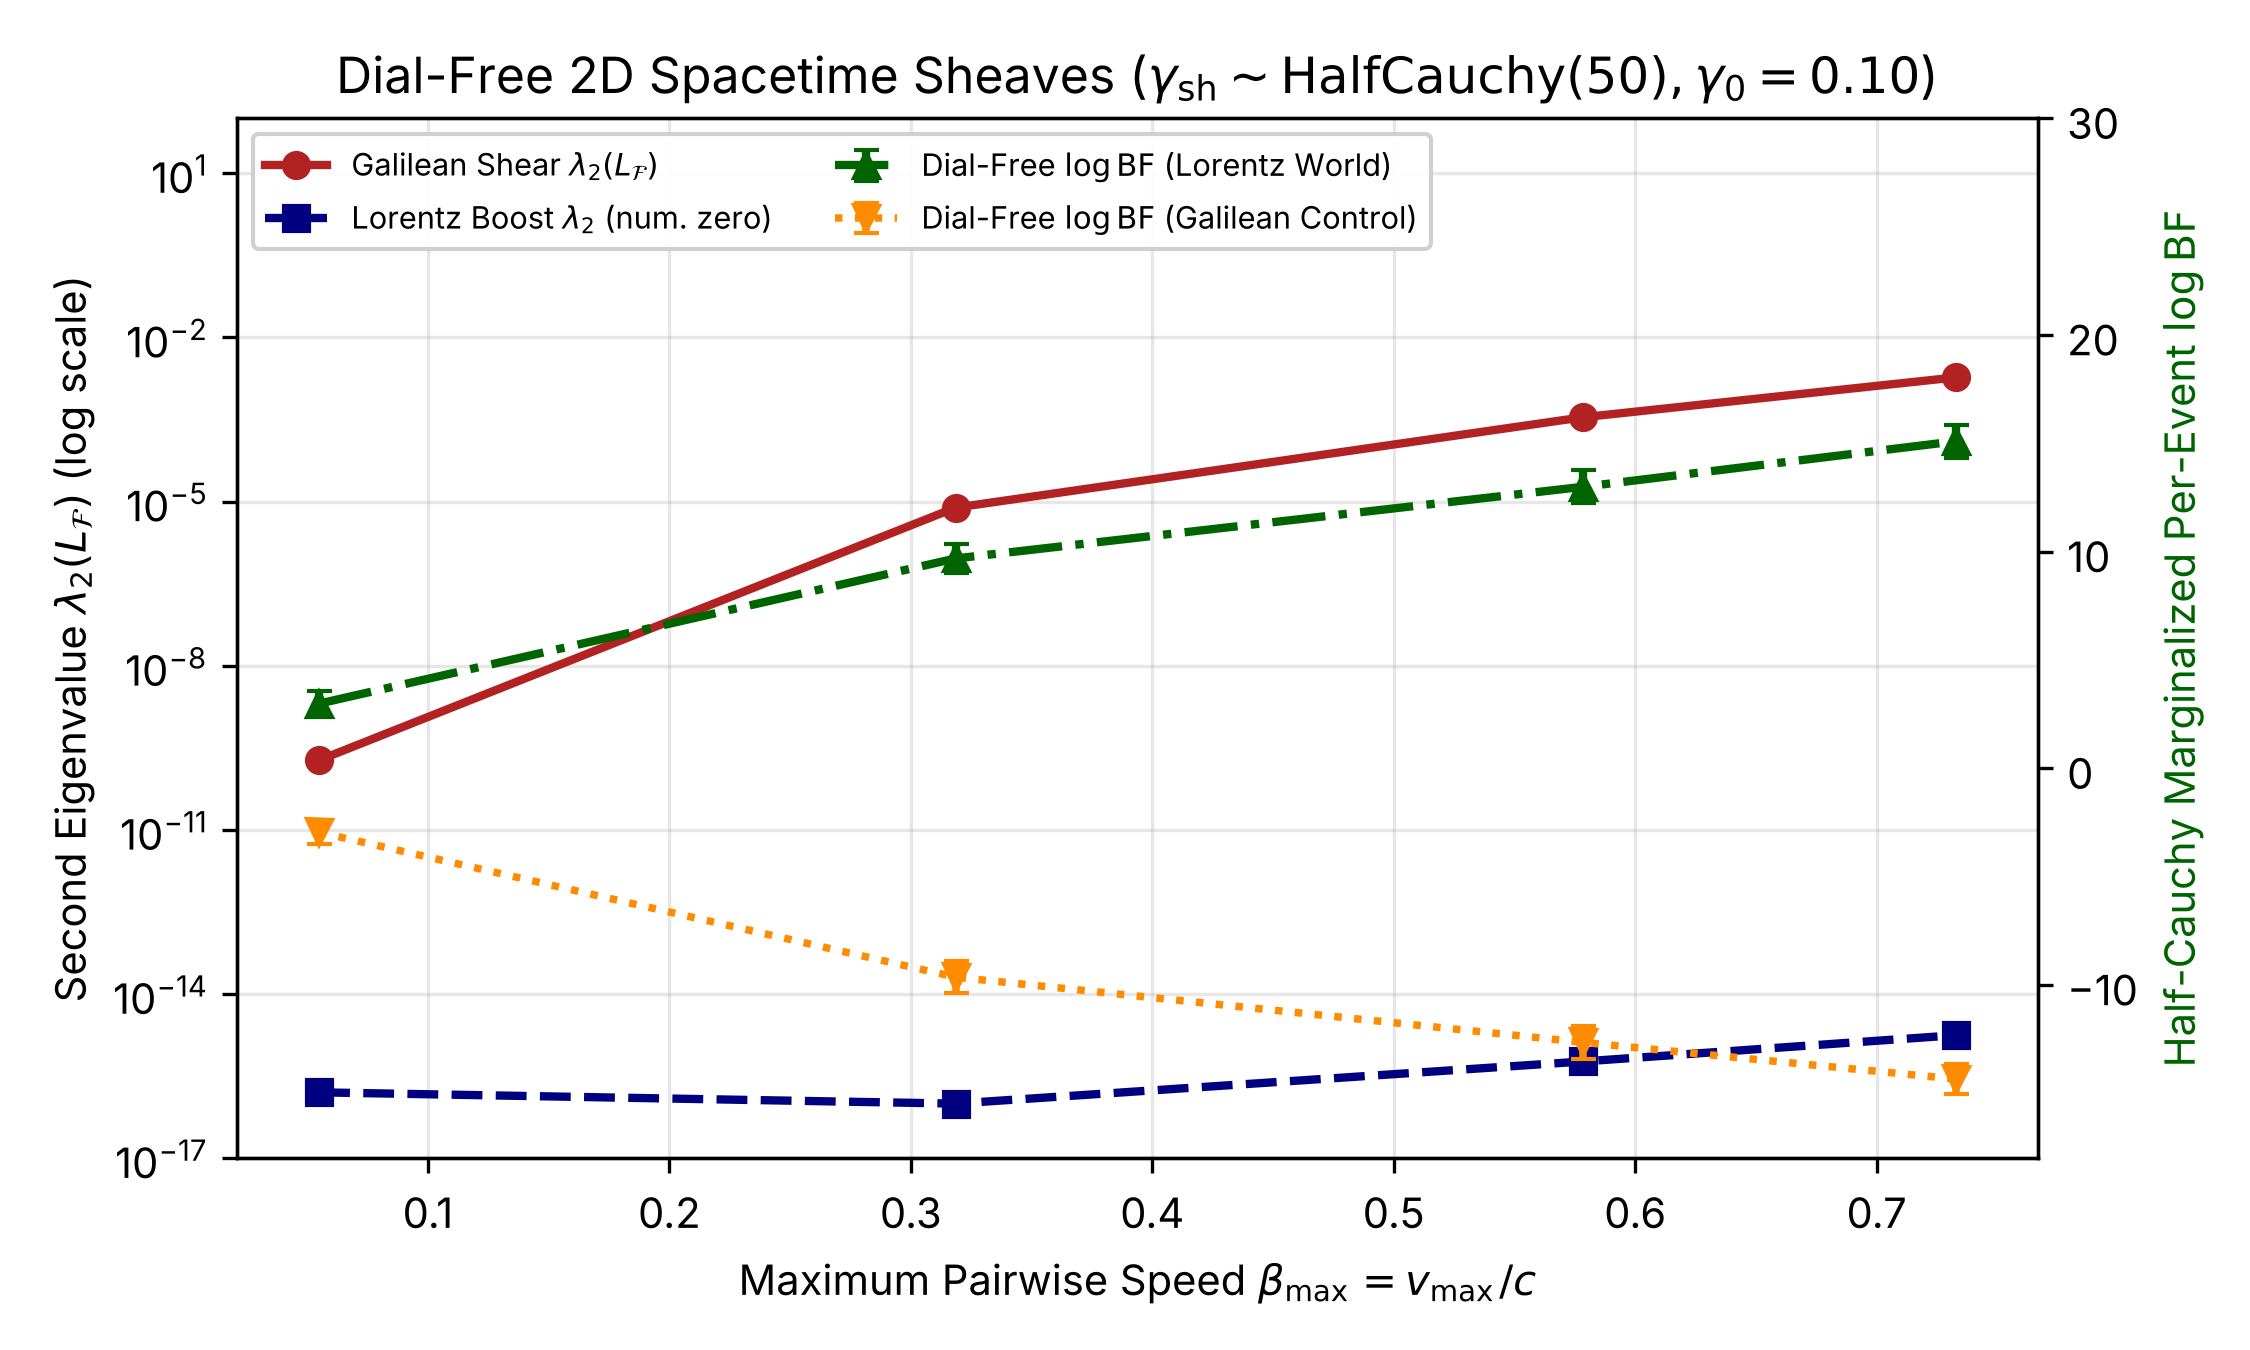
\includegraphics[width=0.74\textwidth]{fig3_spacetime_sheaf_v8_6.png}
  \caption{Dial-free 2D spacetime sheaves ($\gamma_{\mathrm{sh}} \sim \mathrm{HalfCauchy}(50), \gamma_0 = 0.10$): Galilean $\lambda_2(L_{\mathcal{F}})$ vs.\ Lorentz numerical zero ($\approx 10^{-16}$) and symmetric per-event $\log\BF$ in Lorentzian vs.\ Galilean worlds.}
  \label{fig:exp3}
\end{figure}
}{}

\FloatBarrier
\subsection{Experiment 4: Consilience DAG and Objective-by-Sampling Ablation}
\label{sec:exp4}

We construct $12$ theories $M = (\phi_i, w_j)$ over $(z, u) \in \mathbb{Z}_5^2$ combining $3$ feature maps---invariant $\phi_0(z, u) = z$, shortcut $\phi_1(z, u) = u$, and entangled $\phi_2(z, u) = (z+u) \bmod 5$---with $4$ laws $w_0(s) = 2s+1$, $w_1(s) = 2s^2+1$, $w_2(s) = 3s+1$, and $w_3(s) = 4s+2 \pmod 5$ under prior $P(M) \propto 2^{-L_{\mathrm{law}}(M)}$, with nominal code lengths $L_{\mathrm{law}} = (2.0, 2.3, 2.0, 2.2)$ bits for $w_0, \dots, w_3$ plus $0.8$ bits for $\phi_2$. These are relative lengths: their Kraft sum is $\resKraftSum$, so the normalized prior matches the lengths of Eq.~\eqref{eq:mdl} only after $\resKraftBits$ bits are added to each. Noisy training examples $(0,0)\mapsto 1$ and $(1,1)\mapsto 3$ ($\epsilon_{\mathrm{data}} = 0.03$) leave four candidates that fit the data equally---$(\phi_0, w_0)$, $(\phi_0, w_1)$, $(\phi_1, w_0)$, and $(\phi_1, w_1)$---among which the prior favours the linear law $w_0$ over $w_1$ by a factor $2^{0.3}$; all are queried on out-of-distribution input $(z,u) = (2,0)$ with answer $a = w_j(\phi_i(2,0)) \in \mathbb{Z}_5$ ($a=0$ for $(\phi_0, w_0)$, $a=4$ for $(\phi_0, w_1)$, and shortcut $a=1$ for $\phi_1$). A pointed DAG generates all $60$ terminal states $(M, a)$ along $120$ trajectories branching either $(\phi_i \to w_j \to a)$ or $(w_j \to \phi_i \to a)$ ($P_B = \tfrac{1}{2}$ at $(M,a)$). Five epistemic angles test $M$: $A$ (\emph{range check}, validity $0.84$ if $\phi_i(2,0) \in \{0,1\}$ else $0.62$ on matching $a$, and $0.02$ on $a \ne w_j(\phi_i(2,0))$, favoring shortcut $a=1$); $B$ (\emph{nuisance invariance}, $0.92$ iff $\phi_i(2,0) = \phi_i(2,3)$ else $0.04$, isolating $\phi_0$ and leaving bimodal $[A,B]$ split between $a=0$ and $a=4$); $C_{\mathrm{lin}}$ (\emph{constant first difference}, $0.92$ iff $w_j(2)-w_j(1) \equiv w_j(1)-w_j(0) \pmod 5$ else $0.04$, selecting $w_0 \implies a=0$); $C_{\mathrm{quad}}$ (\emph{second difference}, $0.92$ iff $w_j(2)-2w_j(1)+w_j(0) \equiv 4 \pmod 5$ else $0.04$, selecting $w_1 \implies a=4$); and $D$ (\emph{dead out-of-scope angle}, identically $0$). Angles $B$, $C_{\mathrm{lin}}$ and $C_{\mathrm{quad}}$ assign validity $0$ to any answer $a \ne w_j(\phi_i(2,0))$.

In Table~\ref{tab:exp4} ($\epsilon_{\mathrm{ang}} = 0.02, c_{\mathrm{abs}} = 0.25, V_{\mathrm{sig}} = 25$), verified signatures block $6\times$ paraphrased $[A]^6$ (\texttt{ABSTAIN}, vs.\ lexical Commit $a=1$), whereas $4\times$ cloned $[A]^4$ with forged distinct IDs crosses Chow's threshold (Commit $a=1$), confirming the shared verifier-soundness boundary. Adding $C_{\mathrm{lin}}$ or $C_{\mathrm{quad}}$ to bimodal $[A, B]$ commits symmetrically to $a=0$ or $a=4$, and scope-gating screens $D$. These decisions are computed from the exact normalized reward, with angle validities and signature IDs assigned by hand. They illustrate the rule; they measure neither verifier soundness, the independence of two accepted proofs, posterior calibration nor realized abstention risk. Table~\ref{tab:exp4_objsamp} deconfounds objective from sampling across $50$ seeds initialized from identical peaked logits ($\mathrm{SD} = 2.5$; $\log Z_{\mathrm{GF}}$ starts at $\log Z_{\mathrm{GF}}^* + \mathcal{N}(0, 1.5^2)$; $B = 64$, $900$ steps): \textbf{exploratory off-policy sampling} (each batch drawn afresh from an equal mixture of the forward policy and the uniform distribution over the $120$ enumerated trajectories, with no replay buffer) lowers the $900$-step error under \emph{either} objective, cutting $[A, B]$ and $[A, B, C_{\mathrm{lin}}]$ $\mathrm{TV}$ from $\resTBOnTVmm \pm \resTBOnSDmm$ ($\resTBOnFailmm\%$ with $\mathrm{TV}>0.1$) and $\resTBOnTVcl \pm \resTBOnSDcl$ ($\resTBOnFailcl\%$) on-policy to $\resGFTVmm \pm \resGFTVmmSD$ ($\resTBOffFailmm\%$) and $\resGFTVcl \pm \resGFTVclSD$ ($\resTBOffFailcl\%$) under Trajectory Balance ($|\log Z_{\mathrm{GF}} - \log Z_{\mathrm{GF}}^*| = \resGFLZerr$, $P_F^\top(a=0) = \resGFPzero$), and from $\resOnRKLTVmm \pm \resOnRKLTVmmSD$ ($\resRKLOnFailmm\%$) and $\resOnRKLTVcl \pm \resOnRKLTVclSD$ ($\resRKLOnFailcl\%$) on-policy to $\resRKLOffTVmm \pm \resRKLOffSDmm$ ($\resRKLOffFailmm\%$) and $\resRKLOffTVcl \pm \resRKLOffSDcl$ ($\resRKLOffFailcl\%$) under importance-weighted Reverse-KL with a self-normalized baseline \cite{malkin2023gflownets}, while Factorized Mean-Field VI stays biased ($\resMFVITVmm \pm \resMFVITVmmSD$ and $\resMFVITVcl \pm \resMFVITVclSD$; exhaustive $60$-cell Tabular VI: $\resTabVITVmm \pm \resTabVITVmmSD$). Both Trajectory Balance arms start $\log Z_{\mathrm{GF}}$ near its exact value, so their final error does not show blind estimation. Restarted from $\log Z_{\mathrm{GF}} = 0$ (the two targets have $\log Z_{\mathrm{GF}}^* = \resLogZmm$ and $\resLogZcl$), the exploratory arm reaches $\mathrm{TV} = \resTBBlindTVmm$ and $\resTBBlindTVcl$ with $|\log Z_{\mathrm{GF}} - \log Z_{\mathrm{GF}}^*| = \resTBBlindLZerr$ on the second. The table reports error after $900$ steps; it does not identify mode starvation as the cause of each failure. Optimizing Eq.~\eqref{eq:nuis_elbo} across $J=4$ sycophantic framings cuts $\JS$ from $\resJSzero$ ($\lambda_{\mathrm{sym}}=0$, ELBO $\resELBOzero$) to $\resJStwo$ ($\lambda_{\mathrm{sym}}=2$, unpenalized ELBO $\resELBOtwo$, penalized objective $\resELBOtwoPen$), with soft answer likelihoods $(0.90, 0.25, 0.85)$ for the three mechanism classes.

\begin{table}[!htbp]
\centering
\caption{Experiment 4(a): Symbolic $60$-state DAG consilience, paraphrased and forged-ID attacks, rival quadratic law, and Chow decisions ($c_{\mathrm{abs}}=0.25$).}
\label{tab:exp4}
\footnotesize
\setlength{\tabcolsep}{4pt}
\begin{tabular}{@{}lccccc@{}}
\toprule
Queried Angles & $P(a=0)$ & $P(a=1)$ & $P(a=4)$ & $\max_a P$ & Chow ($0.75$) \\
\midrule
\resTabConsBody
\bottomrule
\end{tabular}
\end{table}

\begin{table}[!htbp]
\centering
\caption{Experiment 4(b): $2 \times 2$ objective-by-sampling ablation on the $120$-trajectory DAG ($50$ seeds, identical initial logits $\mathrm{SD} = 2.5, B = 64, 900$ steps): $\mathrm{TV}$ to $P_{\mathrm{PoE}}$ (mean $\pm$ SD) and $\%$ of seeds with $\mathrm{TV} > 0.1$.}
\label{tab:exp4_objsamp}
\footnotesize
\setlength{\tabcolsep}{4pt}
\begin{tabular}{@{}llcccc@{}}
\toprule
 & & \multicolumn{2}{c}{Bimodal $[A, B]$} & \multicolumn{2}{c}{$[A, B, C_{\mathrm{lin}}]$} \\
\cmidrule(lr){3-4}\cmidrule(l){5-6}
Objective & Sampling & TV & $> 0.1$ & TV & $> 0.1$ \\
\midrule
\resTabObjSampBody
\bottomrule
\end{tabular}
\end{table}

\FloatBarrier
\section{Discussion, Limitations, and Conclusion}
\label{sec:conclusion}

Treated as a Kantian regulative ideal \cite{kant1781critique} rather than unmediated perception of reality in itself \cite{hoffman2019case}, objective truth manifests statistically and topologically as structural invariance across admissible transformations, independent provenance blocks, consilient epistemic angles, and overlapping domain sheaves. Three explicit structural boundaries govern scaling: (1) because forged-ID attacks break both Layer-1 provenance clustering and Layer-2 angle deduplication, the architecture depends on the soundness of $\Valid_M$, which would have to be anchored in formal proof checkers and behavioural faithfulness tests \cite{turpin2023language,lanham2023measuring} and evaluated on TruthfulQA \cite{lin2022truthfulqa}, DomainBed \cite{gulrajani2021search}, WILDS \cite{koh2021wilds}, and live multi-LLM councils \cite{perplexity2026council}; none of that is attempted here; (2) the two-stage $H^0_{\tau_{\mathrm{harm}}}$-centred, likelihood-exponent Student-$t$ filter resists capture by gross faults only when $S_{\mathrm{fault}} < S_{\mathrm{hon}}$ ($\lfloor(N-1)/2\rfloor$ unweighted \cite{lopuhaa1991breakdown}) and the offset clears a margin over the honest residual scale, which is the Student-$t$ core near the origin and, on the one graph and two shifts tested, roughly ten to fifteen times $\sigma_{\mathrm{map}}\|x_{*,v}\|_2$ away from it. Contiguous moderate errors inside the graph-cut core, unverified majorities without enough verified honest sources, and sections large enough that the map discrepancy exceeds the observation noise---where pooling through estimated maps is worse than not pooling unless the coupling admits the map error, as in the three-stage variant, which is given the map-noise scale and loses accuracy and robustness when that scale is set too low (Table~\ref{tab:exp2_ingr})---require upstream provenance signals, map-aware coupling, or active interventions; and (3) every experiment here is small and synthetic ($N = 20$ sources, $60$ states), the $\lfloor(N-1)/2\rfloor$ rule has been tested at that one size, and scaling beyond subset-DP, dense eigensolvers, and uniform sampling of an enumerated trajectory set requires amortized partition samplers, sparse iterative harmonic bases, and tempered off-policy exploration. Two limits of scope stand beside these: an oracle supplies the verifier $\Valid_M$ and the signature IDs in every experiment, so none measures verifier soundness, posterior calibration or realized abstention risk, and a sound checker can still accept two proofs that share their evidence; and the design rule Eq.~\eqref{eq:boed} and the continual filter Eq.~\eqref{eq:continual} are architectural components that Section~\ref{sec:experiments} does not benchmark, so their end-to-end effect is untested. Uniting Lopez-Paz's invariance thesis \cite{lopezpaz2026against} with hierarchical testimony saturation, exploratory GFlowNets, and harmonically centred heavy-tailed sheaves yields a concrete, testable blueprint for superintelligent truth discernment---even against all surface likelihood.

\section*{Methodology and AI Collaboration}
This manuscript was conceived, directed, and edited by Rafael Espericueta. It was developed with two AI systems working in alternating drafting and refereeing roles, and was refereed blind by a third. Gemini (Google) drafted Versions~1--7, contributing mathematical derivations, the unified Bayesian and cellular-sheaf formulation, the \LaTeX{} preparation, and the simulation script through Version~6. Claude (Anthropic) refereed Versions~1--7 with independent reimplementations of the experiments and bibliographic auditing, and contributed the $H^0_{\tau_{\mathrm{harm}}}$ centring stage, the EM odds-contraction analysis behind Proposition~\ref{prop:warm_start}, likelihood-exponent provenance deduplication, the distance, coupling and capture sweeps, and the $2 \times 2$ objective-by-sampling ablation adopted in Version~7. For Version~8 Claude revised the manuscript and the simulation script: the exponent-weighted Stage~1, the three-stage variant, the offset-ratio, verified-source-boundary and combined-filter experiments, the exact two-step decision rates, and the rewording of claims to match those results. Gemini then refereed Version~8, auditing its proofs and its simulation code, and contributed the concave-majorization proof of Theorem~\ref{thm:robust}(1), the direct proof of Proposition~\ref{prop:davis_kahan}(2), the $\gamma_0\Delta^2$ condition of Proposition~\ref{prop:warm_start}, and the block-count heuristic for the verified-source boundary. Claude checked each point, reworded or declined Gemini's other proposals, and prepared Version~8.1 without changing the simulation script or its exported numbers. For Version~8.2 Claude added the ingredient experiment of Table~\ref{tab:exp2_ingr} to the script, leaving every earlier exported number unchanged. Gemini then audited Version~8.2, and Version~8.3 corrected one symbol in the abstract that the audit found inconsistent with the body. The author re-ran the simulation scripts of Versions~8 and~8.2 on his own machine and reproduced every exported number exactly. A copy of Version~8.4 with its version history and collaborators removed was then refereed blind by ChatGPT (OpenAI), which re-executed the simulation script, reproduced its exported numbers, and found that sampling noise in the Layer-1 Gibbs chains had put one near-parity cell of Table~\ref{tab:exp2_bound} on the wrong side of parity. Its report listed $25$ findings in all, among them several overstated claims, two limits of the solvers that the manuscript had not disclosed, and inaccurate descriptions of Experiments~3 and~4. Gemini consolidated those findings and contributed the exact count dynamic programme. Claude verified each point with independent code, replaced the sampler by exact partition marginalization, and prepared Version~8.5 from that digest. The full text of ChatGPT's report reached Claude only afterwards. Claude then prepared Version~8.6, which answers the points that the digest had shortened or omitted, with further checks added to the script and no earlier exported number changed. Gemini audited Version~8.6 and accepted it without conditions, and the author re-ran its script on his own machine and reproduced every exported number exactly. Version~8.7 changes this statement only; its script, exported numbers and figures are those of Version~8.6. The manuscript has not undergone human peer review.

\begin{thebibliography}{99}
\bibitem{abramsky2011cohomology} S.~Abramsky, S.~Mansfield, and R.~S. Barbosa. The cohomology of non-locality and contextuality. In \emph{Proc.\ QPL 2011}, volume~95 of \emph{EPTCS}, pages 1--14, 2012.
\bibitem{ahuja2024provable} K.~Ahuja and A.~Mansouri. On provable length and compositional generalization. \emph{arXiv preprint arXiv:2402.04875}, 2024.
\bibitem{aldous1985exchangeability} D.~J. Aldous. Exchangeability and related topics. In \emph{\'Ecole d'\'Et\'e de Probabilit\'es de Saint-Flour XIII---1983}, volume 1117 of \emph{Lecture Notes in Mathematics}, pages 1--198. Springer, 1985.
\bibitem{arjovsky2019invariant} M.~Arjovsky, L.~Bottou, I.~Gulrajani, and D.~Lopez-Paz. Invariant risk minimization. \emph{arXiv preprint arXiv:1907.02893}, 2019.
\bibitem{arora2023ask} S.~Arora, A.~Narayan, M.~F. Chen, L.~Orr, N.~Guha, K.~Bhatia, I.~Chami, F.~Sala, and C.~R\'e. Ask me anything: A simple strategy for prompting language models. In \emph{ICLR}, 2023.
\bibitem{bartlett1957comment} M.~S. Bartlett. A comment on {D.\ V.\ Lindley's} statistical paradox. \emph{Biometrika}, 44(3/4):533--534, 1957.
\bibitem{beery2018recognition} S.~Beery, G.~Van~Horn, and P.~Perona. Recognition in terra incognita. In \emph{ECCV}, pages 472--489, 2018.
\bibitem{bengio2025scientist} Y.~Bengio, M.~K. Cohen, D.~Fornasiere, J.~Ghosn, et~al. Superintelligent agents pose catastrophic risks: Can scientist {AI} offer a safer path? \emph{arXiv preprint arXiv:2502.15657}, 2025.
\bibitem{born1953physical} M.~Born. Physical reality. \emph{The Philosophical Quarterly}, 3(11):139--149, 1953.
\bibitem{bottou2025fiction} L.~Bottou and B.~Sch\"olkopf. The fiction machine. \emph{SIAM News}, 58(3), 2025.
\bibitem{bovens2003bayesian} L.~Bovens and S.~Hartmann. \emph{Bayesian Epistemology}. Oxford University Press, 2003.
\bibitem{cartwright1983laws} N.~Cartwright. \emph{How the Laws of Physics Lie}. Oxford University Press, 1983.
\bibitem{cassirer1923substance} E.~Cassirer. \emph{Substance and Function, and Einstein's Theory of Relativity}. Open Court, Chicago, 1923.
\bibitem{chen2023universal} X.~Chen, R.~Aksitov, U.~Alon, J.~Ren, K.~Xiao, P.~Yin, S.~Prakash, C.~Sutton, X.~Wang, and D.~Zhou. Universal self-consistency for large language model generation. \emph{arXiv preprint arXiv:2311.17311}, 2023.
\bibitem{chow1970optimum} C.~K. Chow. On optimum recognition error and reject tradeoff. \emph{IEEE Transactions on Information Theory}, 16(1):41--46, 1970.
\bibitem{churchland1979scientific} P.~M. Churchland. \emph{Scientific Realism and the Plasticity of Mind}. Cambridge University Press, 1979.
\bibitem{curie1894symetrie} P.~Curie. Sur la sym\'etrie dans les ph\'enom\`enes physiques, sym\'etrie d'un champ \'electrique et d'un champ magn\'etique. \emph{Journal de Physique Th\'eorique et Appliqu\'ee}, 3(1):393--415, 1894.
\bibitem{dawid1979maximum} A.~P. Dawid and A.~M. Skene. Maximum likelihood estimation of observer error-rates using the {EM} algorithm. \emph{Applied Statistics}, 28(1):20--28, 1979.
\bibitem{deleu2022bayesian} T.~Deleu, A.~G\'ois, C.~Emezue, M.~Rankawat, S.~Lacoste-Julien, S.~Bauer, and Y.~Bengio. Bayesian structure learning with generative flow networks. In \emph{UAI}, pages 518--528, 2022.
\bibitem{dong2009integrating} X.~L. Dong, L.~Berti-\'Equille, and D.~Srivastava. Integrating conflicting data: The role of source dependence. \emph{Proceedings of the VLDB Endowment}, 2(1):550--561, 2009.
\bibitem{elazar2021measuring} Y.~Elazar, N.~Kassner, S.~Ravfogel, A.~Ravichander, E.~Hovy, H.~Sch\"utze, and Y.~Goldberg. Measuring and improving consistency in pretrained language models. \emph{Transactions of the Association for Computational Linguistics}, 9:1012--1031, 2021.
\bibitem{ellis2021dreamcoder} K.~Ellis, C.~Wong, M.~Nye, M.~Sabl\'e-Meyer, L.~Morales, L.~Hewitt, L.~Cary, A.~Solar-Lezama, and J.~B. Tenenbaum. {DreamCoder}: Bootstrapping inductive program synthesis with wake-sleep library learning. In \emph{PLDI}, pages 835--850, 2021.
\bibitem{farquhar2024detecting} S.~Farquhar, J.~Kossen, L.~Kuhn, and Y.~Gal. Detecting hallucinations in large language models using semantic entropy. \emph{Nature}, 630:625--630, 2024.
\bibitem{french2001symmetry} S.~French. Symmetry, structure, and the constitution of objects. \emph{PhilSci-Archive preprint}, 2001. \url{https://philsci-archive.pitt.edu/327/}.
\bibitem{gaukroger2012objectivity} S.~Gaukroger. \emph{Objectivity: A Very Short Introduction}. Oxford University Press, 2012.
\bibitem{gebhart2023knowledge} T.~Gebhart, J.~Hansen, and P.~Schrater. Knowledge sheaves: A sheaf-theoretic framework for knowledge graph embedding. In \emph{AISTATS}, volume 206 of \emph{PMLR}, pages 9094--9116, 2023.
\bibitem{geiger2025priors} B.~C. Geiger and R.~Kern. On the role of priors in {B}ayesian causal learning. \emph{IEEE Transactions on Artificial Intelligence}, 2025. DOI: 10.1109/TAI.2024.3522867 (\emph{arXiv:2504.01424}).
\bibitem{gulrajani2021search} I.~Gulrajani and D.~Lopez-Paz. In search of lost domain generalization. In \emph{ICLR}, 2021.
\bibitem{gunn2016too} L.~J. Gunn, F.~Chapeau-Blondeau, M.~D. McDonnell, B.~R. Davis, A.~Allison, and D.~Abbott. Too good to be true: When overwhelming evidence fails to convince. \emph{Proceedings of the Royal Society A}, 472(2187):20150748, 2016.
\bibitem{guo2023causal} S.~Guo, V.~T\'oth, B.~Sch\"olkopf, and F.~Husz\'ar. Causal de {F}inetti: On the identification of invariant causal structure in exchangeable data. In \emph{NeurIPS}, volume~36, 2023.
\bibitem{gupta2024context} S.~Gupta, S.~Jegelka, D.~Lopez-Paz, and K.~Ahuja. Context is environment. In \emph{ICLR}, 2024.
\bibitem{hansen2019toward} J.~Hansen and R.~Ghrist. Toward a spectral theory of cellular sheaves. \emph{Journal of Applied and Computational Topology}, 3(4):315--358, 2019.
\bibitem{hansen2021opinion} J.~Hansen and R.~Ghrist. Opinion dynamics on discourse sheaves. \emph{SIAM Journal on Applied Mathematics}, 81(5):2033--2060, 2021. DOI: 10.1137/20M1341088.
\bibitem{hoffman2019case} D.~D. Hoffman. \emph{The Case Against Reality: Why Evolution Hid the Truth from Our Eyes}. W.~W. Norton \& Company, 2019.
\bibitem{holmes2017assigning} C.~C. Holmes and S.~G. Walker. Assigning a value to a power likelihood in a general {B}ayesian model. \emph{Biometrika}, 104(2):497--503, 2017.
\bibitem{houlsby2011bayesian} N.~Houlsby, F.~Husz\'ar, Z.~Ghahramani, and M.~Lengyel. Bayesian active learning for classification and preference learning. \emph{arXiv preprint arXiv:1112.5745}, 2011.
\bibitem{hu2024amortizing} E.~J. Hu, M.~Jain, E.~Elmoznino, Y.~Kaddar, G.~Lajoie, Y.~Bengio, and N.~Malkin. Amortizing intractable inference in large language models. In \emph{ICLR}, 2024.
\bibitem{jacobs2021invariance} C.~Jacobs. Invariance or equivalence: A tale of two principles. \emph{Synthese}, 199(3--4):9337--9357, 2021.
\bibitem{janzing2010causal} D.~Janzing and B.~Sch\"olkopf. Causal inference using the algorithmic {M}arkov condition. \emph{IEEE Transactions on Information Theory}, 56(10):5168--5194, 2010.
\bibitem{kalai2026evaluating} A.~T. Kalai, O.~Nachum, S.~S. Vempala, and E.~Zhang. Evaluating large language models for accuracy incentivizes hallucinations. \emph{Nature}, 653(8116):1047--1051, 2026.
\bibitem{kamath2021does} P.~Kamath, A.~Tangella, D.~Sutherland, and N.~Srebro. Does invariant risk minimization capture invariance? In \emph{AISTATS}, pages 4069--4077, 2021.
\bibitem{kant1781critique} I.~Kant. \emph{Critique of Pure Reason}. Cambridge University Press, 1998 (original 1781/1787, trans.\ P.~Guyer and A.~W. Wood).
\bibitem{koh2021wilds} P.~W. Koh, S.~Sagawa, H.~Marklund, S.~M. Xie, M.~Zhang, A.~Balsubramani, W.~Hu, M.~Yasunaga, R.~L. Phillips, I.~Gao, et~al. {WILDS}: A benchmark of in-the-wild distribution shifts. In \emph{ICML}, volume 139 of \emph{PMLR}, pages 5637--5664, 2021.
\bibitem{kosso2003symmetry} P.~Kosso. Symmetry, objectivity, and design. In K.~Brading and E.~Castellani, editors, \emph{Symmetries in Physics: Philosophical Reflections}, pages 413--424. Cambridge University Press, 2003.
\bibitem{lanham2023measuring} T.~Lanham, A.~Chen, A.~Radhakrishnan, B.~Steiner, et~al. Measuring faithfulness in chain-of-thought reasoning. \emph{arXiv preprint arXiv:2307.13702}, 2023.
\bibitem{lin2022truthfulqa} S.~Lin, J.~Hilton, and O.~Evans. {TruthfulQA}: Measuring how models mimic human falsehoods. In \emph{ACL}, pages 3214--3252, 2022.
\bibitem{lin2022bayesian} Y.~Lin, H.~Dong, H.~Wang, and T.~Zhang. Bayesian invariant risk minimization. In \emph{CVPR}, pages 16021--16030, 2022.
\bibitem{lindley1956measure} D.~V. Lindley. On a measure of the information provided by an experiment. \emph{The Annals of Mathematical Statistics}, 27(4):986--1005, 1956.
\bibitem{lindley1957statistical} D.~V. Lindley. A statistical paradox. \emph{Biometrika}, 44(1/2):187--192, 1957.
\bibitem{liu1995ml} C.~Liu and D.~B. Rubin. {ML} estimation of the $t$ distribution using {EM} and its extensions, {ECM} and {ECME}. \emph{Statistica Sinica}, 5(1):19--39, 1995.
\bibitem{lopezpaz2026against} D.~Lopez-Paz. Against all likelihood. \emph{arXiv preprint arXiv:2611.09385}, 2026.
\bibitem{lopuhaa1991breakdown} H.~P. Lopuha\"a and P.~J. Rousseeuw. Breakdown points of affine equivariant estimators of multivariate location and covariance matrices. \emph{The Annals of Statistics}, 19(1):229--248, 1991.
\bibitem{madaleno2026bhip} F.~Madaleno, P.~J.~V. Sand, F.~C. Pereira, and S.~H. Garrido~Mejia. Bayesian hierarchical invariant prediction. In \emph{Proc.\ CLeaR}, volume 323 of \emph{PMLR}, pages 324--352, 2026.
\bibitem{malkin2022trajectory} N.~Malkin, M.~Jain, E.~Bengio, C.~Sun, and Y.~Bengio. Trajectory balance: Improved credit assignment in {GFlowNets}. In \emph{NeurIPS}, volume~35, pages 5955--5967, 2022.
\bibitem{malkin2023gflownets} N.~Malkin, S.~Lahlou, T.~Deleu, X.~Ji, E.~Hu, K.~Everett, D.~Zhang, and Y.~Bengio. {GFlowNets} and variational inference. In \emph{ICLR}, 2023.
\bibitem{manakul2023selfcheckgpt} P.~Manakul, A.~Liusie, and M.~J.~F. Gales. {SelfCheckGPT}: Zero-resource black-box hallucination detection for generative large language models. In \emph{EMNLP}, pages 9004--9017, 2023.
\bibitem{minkowski1952space} H.~Minkowski. Space and time. In \emph{The Principle of Relativity}, pages 73--91. Dover, 1952.
\bibitem{nagel1986view} T.~Nagel. \emph{The View from Nowhere}. Oxford University Press, 1986.
\bibitem{nozick2001invariances} R.~Nozick. \emph{Invariances: The Structure of the Objective World}. Harvard University Press, 2001.
\bibitem{olsson2005against} E.~J. Olsson. \emph{Against Coherence: Truth, Probability, and Justification}. Oxford University Press, 2005.
\bibitem{pearl2023interview} J.~Pearl. {J}udea {P}earl, {AI}, and causality: What role do statisticians play? \emph{Amstat News}, Issue 555, September 2023. Interview by Dana Mackenzie.
\bibitem{perplexity2026council} Perplexity. Introducing {M}odel {C}ouncil, February 2026. \url{https://www.perplexity.ai/hub/blog/introducing-model-council}.
\bibitem{peters2016causal} J.~Peters, P.~B\"uhlmann, and N.~Meinshausen. Causal inference by using invariant prediction: Identification and confidence intervals. \emph{Journal of the Royal Statistical Society: Series B}, 78(5):947--1012, 2016.
\bibitem{pezeshki2024discovering} M.~Pezeshki, D.~Bouchacourt, M.~Ibrahim, N.~Ballas, P.~Vincent, and D.~Lopez-Paz. Discovering environments with {XRM}. In \emph{ICML}, pages 40551--40569, 2024.
\bibitem{pitman2006combinatorial} J.~Pitman. \emph{Combinatorial Stochastic Processes}, volume 1875 of \emph{Lecture Notes in Mathematics (\'Ecole d'\'Et\'e de Probabilit\'es de Saint-Flour XXXII---2002)}. Springer, Berlin, 2006.
\bibitem{poincare1905science} H.~Poincar\'e. \emph{Science and Hypothesis}. Walter Scott Publishing, London, 1905.
\bibitem{popper1959logic} K.~R. Popper. \emph{The Logic of Scientific Discovery}. Hutchinson, 1959.
\bibitem{rosenfeld2021risks} E.~Rosenfeld, P.~Ravikumar, and A.~Risteski. The risks of invariant risk minimization. In \emph{ICLR}, 2021.
\bibitem{saunders2003physics} S.~Saunders. Physics and {L}eibniz's principles. In K.~Brading and E.~Castellani, editors, \emph{Symmetries in Physics: Philosophical Reflections}, pages 289--308. Cambridge University Press, 2003.
\bibitem{soudry2018implicit} D.~Soudry, E.~Hoffer, M.~S. Nacson, S.~Gunasekar, and N.~Srebro. The implicit bias of gradient descent on separable data. \emph{Journal of Machine Learning Research}, 19(70):1--57, 2018.
\bibitem{theis2016note} L.~Theis, A.~van~den Oord, and M.~Bethge. A note on the evaluation of generative models. In \emph{ICLR}, 2016.
\bibitem{turpin2023language} M.~Turpin, J.~Michael, E.~Perez, and S.~Bowman. Language models don't always say what they think: Unfaithful explanations in chain-of-thought prompting. In \emph{NeurIPS}, 2023.
\bibitem{ursic2006einstein} M.~Ur\v{s}i\v{c}. Einstein on religion and science. \emph{Synthesis Philosophica}, 21(2):267--283, 2006.
\bibitem{vanfraassen1989laws} B.~C. van Fraassen. \emph{Laws and Symmetry}. Oxford University Press, 1989.
\bibitem{velickovic2026perplexity} P.~Veli\v{c}kovi\'c, F.~Barbero, C.~Perivolaropoulos, S.~Osindero, and R.~Pascanu. Perplexity cannot always tell right from wrong. \emph{arXiv preprint arXiv:2601.22950}, 2026.
\bibitem{wang2023selfconsistency} X.~Wang, J.~Wei, D.~Schuurmans, Q.~Le, E.~Chi, S.~Narang, A.~Chowdhery, and D.~Zhou. Self-consistency improves chain of thought reasoning in language models. In \emph{ICLR}, 2023.
\bibitem{wang2024unleashing} Z.~Wang, S.~Mao, W.~Wu, T.~Ge, F.~Wei, and H.~Ji. Unleashing the emergent cognitive synergy in large language models: A task-solving agent through multi-persona self-collaboration. In \emph{NAACL}, pages 257--279, 2024.
\bibitem{wedin1972perturbation} P.-\AA. Wedin. Perturbation bounds in connection with singular value decomposition. \emph{BIT Numerical Mathematics}, 12(1):99--111, 1972.
\bibitem{weiszfeld1937point} E.~Weiszfeld. Sur le point pour lequel la somme des distances de $n$ points donn\'es est minimum. \emph{T\^ohoku Mathematical Journal, First Series}, 43:355--386, 1937.
\bibitem{weyl1912asymptotische} H.~Weyl. Das asymptotische {V}erteilungsgesetz der {E}igenwerte linearer partieller {D}ifferentialgleichungen (mit einer {A}nwendung auf die {T}heorie der {H}ohlraumstrahlung). \emph{Mathematische Annalen}, 71(4):441--479, 1912.
\bibitem{weyl1952symmetry} H.~Weyl. \emph{Symmetry}. Princeton University Press, 1952.
\bibitem{whewell1840philosophy} W.~Whewell. \emph{The Philosophy of the Inductive Sciences, Founded Upon Their History}. John W.\ Parker, London, 1840.
\bibitem{wigner1967symmetries} E.~P. Wigner. \emph{Symmetries and Reflections: Scientific Essays of Eugene P.\ Wigner}. Indiana University Press, 1967.
\bibitem{woodward2003making} J.~Woodward. \emph{Making Things Happen: A Theory of Causal Explanation}. Oxford University Press, 2003.
\bibitem{worrall1989structural} J.~Worrall. Structural realism: The best of both worlds? \emph{Dialectica}, 43(1--2):99--124, 1989.
\bibitem{xiao2021bit} Z.~Xiao, J.~Shen, X.~Zhen, L.~Shao, and C.~G.~M. Snoek. A bit more {B}ayesian: Domain-invariant learning with uncertainty. In \emph{ICML}, volume 139 of \emph{PMLR}, pages 11351--11361, 2021.
\bibitem{yohai1987high} V.~J. Yohai. High breakdown-point and high efficiency robust estimates for regression. \emph{The Annals of Statistics}, 15(2):642--656, 1987.
\bibitem{yuan2023revisiting} L.~Yuan, Y.~Chen, G.~Cui, H.~Gao, F.~Zou, X.~Cheng, H.~Ji, Z.~Liu, and M.~Sun. Revisiting out-of-distribution robustness in {NLP}: Benchmarks, analysis, and {LLMs} evaluations. In \emph{NeurIPS}, volume~36, pages 58478--58507, 2023.
\bibitem{zhou2022sparse} X.~Zhou, Y.~Lin, W.~Zhang, and T.~Zhang. Sparse invariant risk minimization. In \emph{ICML}, volume 162 of \emph{PMLR}, pages 27222--27244, 2022.
\end{thebibliography}

\end{document}

